\newpage
~
\newpage
\chapter{Propuesta}
Dado que se trata de un TFG de desarrollo, se describe lo realizado, el procedimiento seguido y los resultados obtenidos.

Una vez analizado el estado del arte y las tecnologías disponibles, se propone una propuesta a desarrollar que busca cumplir con los objetivos planteados en la introducción. Para el desarrollo de la propuesta se utilizan metodologías ágiles y tecnologías modernas para garantizar un desarrollo eficiente y que permitirá una fácil adaptación a los cambios que puedan surgir durante el desarrollo del proyecto.

Tal como se ha especificado en los capítulos anteriores, se desarrollará una solución que busca ofrecer:
\begin{itemize}
    \item Solución FOSS que permita aportar al proyecto de manera sencilla, facilitando entender el código y la arquitectura del sistema, consiguiendo de esta manera que sea más fácil contribuir al proyecto.
    \item Soluciones eficientes y rápidas. Para ello se emplearán tecnologías lo más eficientes posibles, siempre buscando la seguridad y escalabilidad de la aplicación.
    \item Solución escalable y mantenible. Se busca que la solución sea escalable y mantenible a largo plazo, permitiendo añadir nuevas funcionalidades y mejoras de manera sencilla. Para ello se implementará una arquitectura limpia \parencite{uncle-bob-clean-architecture}, lo que proporcionará una estructura del proyecto completamente desacoplada, facilitando la escalabilidad y mantenimiento.
    \item Almacenamiento eficiente. Se busca que el almacenamiento de los archivos sea lo más eficiente posible, tanto en términos de espacio como de velocidad de acceso.
        Para ello, primero se hará uso de un sistema de almacenamiento de objetos compatible con \gls{s3}, lo que permitirá utilizar cualquier servicio de almacenamiento compatible con el mismo protocolo como Google Cloud Storage o usando software libre como podría ser \gls{minio}.
        Dada la naturaleza de este proyecto, se utilizará MinIO como solución para el almacenamiento, ya que nos va a permitir almacenar nuestros archivos de manera eficiente en nuestro propio servidor.
        En una ampliación futura se valorará la implementación de una solución de almacenamiento nativa que permita un acceso más rápido y eficiente a los archivos, además de una mejor gestión de los mismos.
    \item Desarrollo ágil y flexible. Se busca que el desarrollo sea ágil y flexible, permitiendo adaptarse a los cambios y necesidades del proyecto de manera rápida y eficiente. Para ello se hará uso de la metodología ágil Scrum, lo que facilitará una organización clara del proyecto y una planificación adecuada de las tareas a realizar.
        Seguir esta metodología favorecerá una mejor organización del proyecto y una planificación adecuada de las tareas a realizar, lo que aportará una buena organización en caso de que se incorporen más personas al proyecto en el futuro.
\end{itemize}

\section{Metodología}
\label{sec:metodologia}

Para el desarrollo de este proyecto se ha optado por la metodología ágil Scrum. Esta metodología se basa en el desarrollo iterativo e incremental, lo que permite una mayor flexibilidad y adaptación a los cambios durante el proceso de desarrollo.

La elección de Scrum sobre otras metodologías ágiles como Kanban o XP (Extreme Programming), o incluso enfoques tradicionales, se fundamenta en la experiencia previa del equipo de desarrollo con este marco de trabajo, lo que garantiza una mayor comodidad y eficacia en su aplicación.
Además, Scrum es una metodología que se adapta muy bien a proyectos de desarrollo de software, ya que permite una mayor flexibilidad y adaptación a los cambios durante el proceso de desarrollo.

Tal y como se explica en la guía oficial de Scrum \parencite{scrum-guide}, Scrum es un marco de trabajo ágil que se utiliza para gestionar proyectos complejos y adaptarse a los cambios de manera rápida y eficiente. Se basa en la colaboración entre equipos multidisciplinarios, la entrega continua de valor y la mejora continua.
Scrum se centra en la entrega de incrementos de producto funcionales en ciclos cortos, lo que permite a los equipos recibir retroalimentación temprana y ajustar su enfoque según sea necesario. Esto es especialmente útil en proyectos donde los requisitos pueden cambiar con frecuencia o donde la incertidumbre es alta.

Scrum se basa en una serie de roles, eventos y artefactos que ayudan a los equipos a organizar su trabajo y colaborar de manera efectiva. Los roles incluyen el Product Owner (responsable de la visión del producto), el Scrum Master (facilitador del proceso) y el equipo de desarrollo (responsable de la entrega del producto). Los eventos incluyen las reuniones diarias, las revisiones de sprint y las retrospectivas, que permiten a los equipos reflexionar sobre su trabajo y mejorar continuamente.

Aunque Scrum está muy enfocado a equipos, también es posible utilizarlo con un equipo muy pequeño o incluso con una sola persona, realizando los mismos eventos pero sin la necesidad de tener un equipo de desarrollo.
Éste es el enfoque que se le va a dar a este proyecto. Una buena práctica de Scrum es documentar todas las reuniones y tomas de decisiones que se toman a lo largo de la vida del proyecto, ya que esto ayuda a tener una mejor organización y a poder ver cómo ha ido evolucionando el proyecto a lo largo del tiempo.
Es por ello que se van a documentar todas las decisiones que se tomen y los cambios que se realicen en el desarrollo.


\begin{figure}[H]
  \centering
  \includegraphics[width=0.8\textwidth]{assets/scrum-diagram.png}
  \caption{Diagrama del proceso completo de Scrum \parencite{scrum-diagram}}
  \label{fig:scrum-diagram}
\end{figure}

En esta imagen se muestra todo el proceso que se sigue con una metodología Scrum, desde la planificación del producto hasta la entrega del mismo.

Como se comenta en la guía de Scrum y se puede ver en la imagen, durante el desarrollo del proyecto se van a generar varios artefactos:
\begin{itemize}
    \item \textbf{Product Backlog}: es una lista priorizada de requisitos o tareas pendientes en un proyecto ágil. En este caso, el product backlog se va a utilizar para organizar todas las historias de usuario e historias técnicas que se van a implementar en el proyecto.
    \item \textbf{Sprint Backlog}: es una lista de tareas (las cuales salen de las historias de usuario y técnicas) seleccionadas del product backlog que se van a realizar durante un sprint.
    \item \textbf{Incremento}: es la suma de todos los elementos del product backlog completados durante un sprint y los incrementos de todos los sprints anteriores. En este caso, el incremento se va a utilizar para organizar todas las tareas que se han realizado durante cada sprint.
\end{itemize}
Aunque el producto sufra cambios después, intentar estimar lo mejor posible y terminar los sprints con un producto con \textbf{valor} es el objetivo principal de esta metodología, tal y como se dice en la guía `\textit{A product is a vehicle to deliver value. It has a clear boundary, known stakeholders, well-defined users or customers. A product could be a service, a physical product, or something more abstract.}' (\cite{scrum-guide}, apartado de Product Backlog)

Se separará el desarrollo en distintos sprints, cada uno de ellos con una duración de dos semanas.

Durante cada sprint se seleccionarán las historias de usuario\footnote{Las historias de usuario son descripciones concisas y sencillas de una funcionalidad, escritas desde la perspectiva del usuario} al principio del sprint y se desarrollarán (posible desglose en distintas historias de usuario, definición de tareas relacionadas con la HU junto con estimación de las mismas y definición de pruebas de aceptación) generando así el Sprint Backlog correspondiente a ese sprint, se completarán las tareas necesarias para completarlas.

Al final del sprint se realizará una revisión en la que se analizará lo que se ha conseguido hacer y si se ha cumplido con lo definido antes del sprint para adaptar el product backlog si fuera necesario y tenerlo en cuenta para el siguiente sprint. En la revisión participarán Product Owner, equipo de desarrollo, Scrum Master y los interesados en el proyecto (Stakeholders). Aquí es donde se presenta el incremento del producto a los interesados y se recibe retroalimentación sobre el trabajo realizado.

Y por último se lleva a cabo una retrospectiva en el equipo, donde se reflexiona principalmente sobre el modo de trabajo, los aspectos positivos, negativos y las posibles mejoras para el siguiente sprint. Esto es una parte fundamental de Scrum, ya que permite al equipo aprender de su experiencia y mejorar continuamente.

Gracias a esta metodología se consigue tener una organización muy clara de lo que se va a hacer, cómo se va a hacer y cuándo se va a hacer.

\section{Sprint 0}
\label{sec:planificacion-inicial}
Durante un desarrollo con Scrum, tal como se ha comentado anteriormente en la \hyperref[sec:metodologia]{sección de metodología}, se usan \textbf{sprints} para dividir el desarrollo en partes organizadas y planificadas con anterioridad, las cuales tienen un inicio y un fin.

Se suele crear un sprint denominado como ``Sprint 0'' en el que se hace una planificación inicial, se genera la que va a ser la primera versión del product backlog y se dan unas estimaciones de las tareas que se van a realizar en todos los sprints.
Durante este sprint no se va a desarrollar funcionalidad, si no que se van a asentar unas bases para todo el proyecto sobre las cuales se trabajará en los siguientes sprints.
Los objetivos de este sprint son los siguientes:

\begin{itemize}
    \item Definir diagrama de la arquitectura inicial del sistema.
    \item Estudiar la estructura de implementación del sistema.
    \item Definir un presupuesto para el proyecto (sección \hyperref[sec:presupuesto]{Presupuesto}).
    \item Definir el product backlog inicial (sección \hyperref[sec:historias-de-usuario]{Historias de usuario}).
    \item Estudiar documentación y cursos de las tecnologías de backend que se van a utilizar.
    \item Estudiar la documentación sobre las tecnologías de frontend que se van a utilizar.
    \item Definir el entorno de desarrollo tanto para el servidor como el cliente.
    \item Definir el backlog de el primer sprint.
    \item Realizar diagrama de Gantt para el primer sprint.
\end{itemize}

El product backlog inicial se ha definido en la \hyperref[sec:historias-de-usuario]{sección de historias de usuario} y se ha dividido en dos partes, una para el servidor y otra para el cliente móvil.

\subsection{Historias de usuario / Historias técnicas}
\label{sec:historias-de-usuario}
En esta sección se detallan las historias de usuario e historias técnicas de la aplicación, separadas en dos grupos: las de la aplicación de servidor y las de móvil.

Se ha considerado esta separación ya que la aplicación de servidor tiene un objetivo diferente al de la aplicación móvil, de esta manera conseguimos una mejor organización de las historias de usuario.

Durante los primeros sprints se trabajará de manera principalmente separada, enfocándose en la parte correspondiente que se defina de la aplicación y en una fase más avanzada se trabajará de manera conjunta, integrando ambas aplicaciones. Se realizará de esta manera para para poder enfocarnos mejor en una sola parte del proyecto, de esta manera no tenemos que estar cambiando de contexto constantemente entre las dos aplicaciones, lo que podría hacer que el desarrollo fuera más lento y tedioso.

Para la planificación del desarrollo se han utilizado puntos de historia (PH), los cuales representan una estimación de lo que se considera que se tardará en implementar las historias de usuario. Esta estimación es relativa, es decir, no representa un tiempo real sino una estimación con respecto a todas las demás historias de usuario, siendo 1 punto de historia la historia de usuario más sencilla de implementar o que menos tiempo requiere.

Este es un listado inicial de historias de usuario, durante los sprints se irá especificando si alguna historia de usuario ha cambiado, añadido o eliminado del product backlog\footnote{El product backlog es una lista priorizada de requisitos o tareas pendientes en un proyecto ágil.}.

Cada historia de usuario tiene un identificador único, una descripción de la historia de usuario y una estimación en puntos de historia. Ésta es después desglosada en historias de usuario más pequeñas de las cuales se definen tareas que tienen que ser realizadas para completar la historia de usuario con su estimación en horas.
Además de las historias de usuario, contamos con historias técnicas, que son historias de usuario que no están relacionadas directamente con el usuario final, sino que son necesarias para el correcto funcionamiento del sistema. Estas historias técnicas se consideran como historias de usuario y se les asigna una estimación en puntos de historia.

A lo largo del product backlog  se hará referencia a HU\{identificador\} para las historias de usuario y HT\{identificador\} para las historias técnicas. El identificador será un número entero que se asignará de manera consecutiva a cada historia de usuario o historia técnica. Para la sub-historias de usuario se asignará un número entero que será el mismo que la historia de usuario a la que pertenece, seguido de un punto y otro número entero que será el identificador de la sub-historia de usuario, por ejemplo: HU1, HU1.1, HU1.2, etc.

\paragraph{Servidor}
\renewcommand{\arraystretch}{1.3} % Increases row height for readability
\rowcolors{2}{gray!15}{white} % Alternate row colors

\begin{tabularx}{\textwidth}{|l|l|>{\raggedright\arraybackslash}X|l|}
    \hline
\textbf{ID} & \textbf{Título} & \textbf{Descripción} & \makecell{\textbf{Estimación}\\\textbf{(PH)}} \\
    \hline
    HU01 & Subida de fotos & Como usuario, quiero subir varias fotos desde mi móvil para tener una copia de seguridad en mi servidor. & 5 \\
    \hline
    HU02 & Estado de sincronización & Como usuario, quiero ver qué fotos están subidas y cuáles no, para saber el estado de sincronización. & 3 \\
    \hline
    HU03 & Eliminar fotos & Como usuario, quiero eliminar fotos subidas desde la app, para liberar espacio en mi servidor. & 3 \\
    \hline
    HU04 & Subida de vídeos & Como usuario, quiero subir vídeos además de fotos, para guardar también mis recuerdos en vídeo. & 5 \\
    \hline
    HU05 & Inicio de sesión & Como usuario, quiero iniciar sesión con contraseña o clave, para evitar que otros accedan a mis archivos. & 5 \\
    \hline
    HU06 & Cerrar sesión & Como usuario, quiero poder cerrar sesión en un dispositivo, para proteger mis datos si pierdo el móvil. & 2 \\
    \hline
    HU07 & Descubrimiento automático & Como usuario, quiero que la app detecte automáticamente mi servidor en la red local, para no tener que configurarlo manualmente. & 8 \\
    \hline
    HU08 & Conexión remota & Como usuario, quiero poder conectarme remotamente si expongo mi servidor, para acceder a mis fotos desde fuera de casa. & 13 \\
    \hline
    HU09 & Galería visual & Como usuario, quiero ver una galería de las fotos y videos subidos, para revisar mi contenido fácilmente. & 5 \\
    \hline
    HU10 & Espacio ocupado & Como usuario, quiero ver el espacio ocupado por mis archivos, para controlar el almacenamiento del servidor. & 3 \\
    \hline
    HU11 & Estadísticas de copia & Como usuario, quiero ver estadísticas de sincronización, para saber cuándo fue la última copia y cuántos archivos se han guardado. & 3 \\
    \hline
    HU12 & Cancelar sincronización & Como usuario, quiero cancelar una sincronización en curso. & 5 \\
    \hline
    HU13 & Crear cuentas & Como administrador, quiero crear cuentas de usuario con permisos, para que varias personas puedan usar el servidor. & 8 \\
    \hline
    HU14 & Galería privada & Como usuario, quiero tener mi propia galería separada de otros usuarios. & 5 \\
    \hline
    HU15 & Galería online & Como usuario, quiero poder ver todas las fotos que tengo en el servidor sin necesidad de tener que descargarlas en mi móvil, tanto las que he subido yo como las que han compartido conmigo. & 8 \\
    \hline
    HT01 & Hash de archivos & Implementar sistema de cálculo de hash para detectar duplicados. & 3 \\
    \hline
    HT02 & Sincronización incremental & Implementar sincronización basada en metadatos (fecha, tamaño, hash). & 5 \\
    \hline
    HT03 & API REST & Desarrollar API RESTful par el servidor & 13 \\
    \hline
    HT04 & Descubrimiento mDNS & Crear sistema de descubrimiento automático usando mDNS. & 8 \\
    \hline
    HT05 & Autenticación JWT & Implementar autenticación con JSON Web Tokens. & 5 \\
    \hline
    HT06 & HTTPS en servidor & Configurar comunicación segura con HTTPS. & 5 \\
    \hline
    HT07 & Estructura de almacenamiento & Definir carpetas y metadatos para organizar los archivos. & 5 \\
    \hline
    HT08 & Base de datos & Implementar SQLite o PostgreSQL para usuarios y archivos. & 8 \\
    \hline
    HT09 & Compresión de imágenes & Implementar compresión para optimizar el almacenamiento. & 5 \\
    \hline
    HT10 & Subida concurrente & Soporte para subida simultánea y manejo de errores. & 8 \\
    \hline
    HT11 & Tests & Añadir pruebas unitarias e integración en backend. & 5 \\
    \hline
    HT12 & CI/CD & Configurar pipelines de integración y despliegue. & 5 \\
    \hline
    HT13 & Logging & Implementar logs detallados para depuración. & 3 \\
    \hline
    HT14 & Cobertura de tests & Medir y asegurar la cobertura de pruebas. & 3 \\
    \hline
    HT15 & Interfaz Tauri & Crear interfaz gráfica del servidor con Tauri. & 8 \\
    \hline
    HT16 & Panel de control & Implementar visualización de archivos y uso del sistema. & 5 \\
    \hline
    HT17 & Notificaciones de progreso & Integrar notificaciones del sistema con progreso de subida. & 3 \\
    \hline
    HT18 & Binario y Tauri & Empaquetar servidor como CLI y app Tauri. & 5 \\
    \hline
    HT19 & Dockerización & Crear imagen Docker del servidor. & 3 \\
    \hline
    HT20 & Documentación & Documentar instalación y uso del sistema. & 13 \\
    \hline
    HT21 & Backups externos & Soporte para backups automáticos externos. & 8 \\
    \hline
    HT22 & Logs persistentes & Configurar sistema de logs persistentes y rotación. & 3 \\
    \hline
\end{tabularx}

\paragraph{Historias que se han dividido}

Ambas tablas que aparecen a continuación muestran historias técnicas que han sido divididas en sub-historias para facilitar su gestión y estimación en el backlog.

\begin{table}[h!]
    \begin{center}
        \begin{tabularx}{\textwidth}{|l|l|>{\raggedright}X|l|}
            \hline
            ID & Título & Descripción & Estimación \\
            \hline
            HT18 & Binario y Tauri & Empaquetar servidor como CLI y app Tauri. & 5 \\
            \hline
            HT18.1 & Binario & Empaquetar la aplicación como un solo binario & 2 \\
            \hline
            HT18.2 & Tauri & Empaquetar aplicación de escritorio con Tauri & 3 \\
            \hline
        \end{tabularx}
    \end{center}
\end{table}

\begin{table}[h!]
    \begin{center}
        \begin{tabularx}{\textwidth}{|l|X|>{\raggedright\arraybackslash}X|l|}
            \hline
            ID & Título & Descripción & Estimación \\
            \hline
            HT20 & Documentación & Documentar instalación y uso del sistema. & 13 \\
            \hline
            HT20.1 & Documentación del proyecto en Github & Documentar la instalación y uso del proyecto en el repositorio de Github & 5 \\
            \hline
            HT20.2 &  Documentación de la API REST con OpenAPI & Documentar mediante la generación de una página web todos los endpoints de la API REST & 5 \\
            \hline
            HT20.3 & Documentación de la aplicación Tauri & Manual de usuario de la aplicación de escritorio desarrollada con Tauri & 3 \\
            \hline
        \end{tabularx}
    \end{center}
\end{table}

\newpage
\paragraph{Móvil}
\begin{tabularx}{\textwidth}{|l|l|>{\raggedright\arraybackslash}X|l|}
    \hline
    ID & Título & Descripción & Estimación \\
    \hline
    HU16 & Seleccionar fotos & Como usuario, quiero seleccionar varias fotos desde mi galería para subirlas al servidor. & 3 \\
    \hline
    HU17 & Subir fotos automáticamente & Como usuario, quiero que se suban automáticamente las nuevas fotos que hago, sin tener que hacerlo manualmente. & 8 \\
    \hline
    HU18 & Ver progreso de subida & Como usuario, quiero ver el progreso de cada archivo que se está subiendo. & 8 \\
    \hline
    HU19 & Cancelar subida & Como usuario, quiero cancelar una subida en curso desde la interfaz. & 3 \\
    \hline
    HU20 & Ver archivos subidos & Como usuario, quiero ver una lista o galería de los archivos que ya están subidos. & 5 \\
    \hline
    HU21 & Conexión automática al servidor & Como usuario, quiero que la app detecte y se conecte automáticamente al servidor en mi red. & 5 \\
    \hline
    HU22 & Cambiar de servidor & Como usuario, quiero poder cambiar manualmente la dirección del servidor si quiero usar otro. & 3 \\
    \hline
    HU23 & Ver uso de almacenamiento & Como usuario, quiero ver cuánto espacio he usado en el servidor. & 3 \\
    \hline
    HU24 & Inicio y cierre de sesión & Como usuario, quiero iniciar y cerrar sesión para proteger mis datos. & 5 \\
    \hline
    HU25 & Gestión de permisos & Como usuario, quiero que la app me pida permisos de acceso solo cuando sea necesario. & 3 \\
    \hline
    HU26 & Notificaciones de subida & Como usuario, quiero recibir notificaciones cuando se complete la sincronización. & 5 \\
    \hline
    HU27 & Subir vídeos & Como usuario, quiero subir también vídeos de mi galería al servidor. & 5 \\
    \hline
    HU28 & Subida en segundo plano & Como usuario, quiero que las subidas continúen aunque cierre la app. & 8 \\
    \hline
    HU29 & Sincronización manual & Como usuario, quiero poder iniciar la sincronización manualmente. & 3 \\
    \hline
    HU30 & Galería online & Como usuario, quiero ver mis fotos en la app sin tener que descargarlas. & 5 \\
    \hline
    HT23 & Acceso a la galería & Implementar acceso seguro a la galería de fotos y vídeos. & 5 \\
    \hline
    HT24 & Comunicación con API & Integrar cliente HTTP que se comunique con el servidor. & 5 \\
    \hline
    HT25 & Almacenamiento local & Guardar estado de archivos subidos/no subidos de forma local. & 3 \\
    \hline
    HT26 & Manejo de errores de red & Implementar gestión de errores de red y reintentos automáticos. & 5 \\
    \hline
    HT27 & Subida concurrente & Soportar subida de varios archivos en paralelo con control de errores. & 5 \\
    \hline
    HT28 & Sincronización de fondo & Implementar sincronización en segundo plano. & 8 \\
    \hline
    HT29 & Pruebas unitarias & Añadir pruebas unitarias y de integración a la lógica común en React Native / Lynx.js & 13 \\
    \hline
    HT30 & CI/CD móvil & Pipeline de construcción y publicación para Android e iOS. & 5 \\
    \hline
    HT31 & Gestión de tokens & Almacenar y renovar tokens de autenticación de forma segura. & 3 \\
    \hline
    HT32 & Notificaciones locales & Integrar sistema de notificaciones locales en Android/iOS. & 3 \\
    \hline
    HT33 & Optimización de red & Reducir uso de red usando compresión. & 5 \\
    \hline
    HT34 & Localización & Soporte multilenguaje para la aplicación. & 8 \\
    \hline
    HT35 & Permisos condicionales & Solicitar permisos en tiempo de ejecución de forma contextual. & 3 \\
    \hline
    HT36 & UI responsive & Adaptar UI para distintos tamaños de pantalla (tablet, móvil). & 3 \\
    \hline
\end{tabularx}



\subsection{Arquitectura del sistema}
\begin{figure}[H]
    \begin{center}
        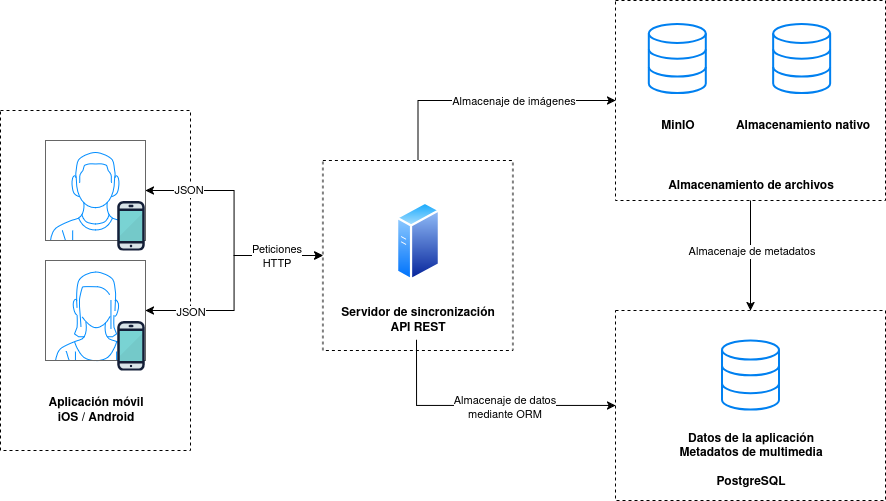
\includegraphics[width=0.95\textwidth]{images/diagrama-arquitectura.png}
    \end{center}
    \caption{Diagrama de la arquitectura del sistema. Representa las comunicaciones entre los distintos elementos del sistema}\label{fig:diagrama-arquitectura}
\end{figure}

Como se muestra en la Figura \ref{fig:diagrama-arquitectura}, el sistema va a estar compuesto por un cliente (móvil tanto en Android como iOS) que se comunica con un servidor mediante peticiones HTTP.
Se estudió la posibilidad de la comunicación mediante gRPC (\textit{Google Remote Procedure Call}) pero se desechó ya que la compatibilidad entre un cliente multiplataforma móvil y el servidor de sincronización no permitía hacer uso de todas las ventajas que ofrecía frente a un método convencional como puede ser una API REST.

Todo esto hizo decidirse por una API REST, la cual es más sencilla de implementar y de mantener a largo plazo, además de ser más fácil de entender para cualquier desarrollador que quiera contribuir al proyecto.

El servidor se comunicará de manera abstracta con un servicio de almacenamiento de datos. Para la primera versión de la aplicación se hará uso de MinIO, un software Open-Source que permite crear un servidor de almacenamiento de objetos compatible con la API de Amazon S3.
Esto proporciona la ventaja de poder utilizar cualquier servicio de almacenamiento compatible con S3 como Amazon S3, Google Cloud Storage en el futuro sin necesidad de cambiar la aplicación.
MinIO está diseñado para ser totalmente escalable y de alto rendimiento, lo que lo convierte en una excelente opción para almacenar grandes volúmenes de datos, como fotos y vídeos.

Aunque en las primeras iteraciones se utilice MinIO para almacenar los datos multimedia, en iteraciones más avanzadas se implementará un sistema de almacenamiento nativo, el cual permitirá un mayor control sobre los datos y una mejor integración con el resto del sistema.

Gracias a la arquitectura limpia (\cite{uncle-bob-clean-architecture}) que se va a utilizar a la hora de implementar el sistema, se consigue un desacople total de la capa de aplicación, dominio e infraestructura, brindando la posibilidad de cambiar la implementación de la capa de infraestructura sin afectar al resto del sistema, proporcionando de esta manera flexibilidad sobre la solución que se desee usar para almacenar los datos/multimedia.

Para el almacenaje de los datos de la aplicación se ha optado por hacer uso de un \acrshort{orm} con PostgreSQL.
Aunque puede ser menos escalable comparado con otras soluciones noSQL a largo plazo, esta opción proporciona una gran cantidad de ventajas frente a las desventajas que tiene, como pueden ser:
\begin{itemize}
    \item \textbf{Integridad de los datos}: PostgreSQL es un sistema de gestión de bases de datos relacional, lo que significa que garantiza la integridad de los datos mediante el uso de transacciones y restricciones.
    \item \textbf{Escalabilidad}: aunque no es tan escalable como otras soluciones noSQL, PostgreSQL es capaz de manejar grandes volúmenes de datos y puede escalar horizontalmente mediante particionamiento.
    \item \textbf{Rendimiento}: PostgreSQL es conocido por su alto rendimiento y eficiencia en el manejo de consultas complejas y grandes volúmenes de datos.
    \item \textbf{Comunidad activa}: PostgreSQL tiene una comunidad muy activa y una gran cantidad de documentación y recursos disponibles, lo que facilita su aprendizaje y uso.
    \item \textbf{Open-Source}: al ser un software Open-Source, no es necesario pagar por licencias y se alinea con el enfoque del proyecto que busca ser Open-Source.
\end{itemize}

Aunque se elija una base de datos en este punto del proyecto, la arquitectura del sistema permite cambiar la implementación de la capa de infraestructura sin afectar al resto del sistema, lo que proporciona flexibilidad para cambiar la base de datos en el futuro si fuera necesario.
Además, se ha optado por hacer uso de un \acrshort{orm} para facilitar la interacción con la base de datos y abstraer la complejidad de las consultas SQL, lo que permite centrarse en la lógica de negocio y no en la implementación de la base de datos.
Esto otorga mayor flexibilidad a la hora de cambiar la base de datos en el futuro, ya que el \acrshort{orm} permite cambiar el motor de base de datos fácilmente.

\subsection{Arquitectura software}
En un proyecto de este tipo es muy importante tener una buena estructura a la hora de diseñar el software.
Se busca la separación de responsabilidades y una buena organización, lo cual satisface uno de los objetivos específicos (OE5): desarrollar un sistema que sea fácilmente escalable.

Para ello, se han estudiado las distintas opciones disponibles, tanto para el servidor como para la aplicación móvil, y se ha optado por una variación de la arquitectura limpia \parencite{uncle-bob-clean-architecture}, cuyos principios son:
\begin{itemize}
    \item \textbf{Separación de responsabilidades}: cada capa del sistema tiene una responsabilidad clara y bien definida, lo que facilita el mantenimiento y la evolución del sistema.
    \item \textbf{Independencia de la infraestructura}: las capas más internas del sistema no dependen de detalles de implementación de la infraestructura, lo que permite cambiar la infraestructura sin afectar al resto del sistema.
    \item \textbf{Facilidad de pruebas}: al tener una separación clara de responsabilidades, es más fácil realizar pruebas unitarias e integración, lo que mejora la calidad del software.
    \item \textbf{Escalabilidad}: al estar desacopladas las distintas capas del sistema, es más fácil escalar el sistema a medida que crece.
\end{itemize}

\paragraph{Arquitectura del servidor}
\subparagraph{}
Para el servidor se ha decidido usar una estructura monolítica modular siguiendo los principios de una arquitectura limpia.
Este enfoque se acerca a lo que sería una estructura de microservicios, pero sin la complejidad que conlleva el uso de múltiples servicios.
Siguiendo esta solución la aplicación se compone de un solo binario que contiene todo el código del servidor, pero con una estructura modular donde cada módulo tiene una responsabilidad clara y bien definida.
Es la mejor solución para un equipo pequeño ya que se elimina el factor de la comunicación entre distintos servicios, el despliegue de los mismos y la gestión de la infraestructura para cada uno de los servicios.

Aun así, cuenta con la gran mayoría de las ventajas que proporciona una arquitectura de microservicios, como la separación de responsabilidades, la facilidad de pruebas y la escalabilidad.
De esta manera, en un futuro se podría separar el servidor en microservicios de manera sencilla, dado que se dispone de una estructura modular donde cada módulo tiene su responsabilidad, por lo que tan solo sería necesario separar los módulos en distintos servicios y hacer que se comuniquen entre ellos mediante un protocolo de comunicación específico, como puede ser HTTP o gRPC.


\begin{figure}[H]
  \centering
  \includegraphics[width=0.8\textwidth]{assets/modular-monolith-comparison.png}
  \caption{Comparativa entre una arquitectura monolítica, de microservicios y monolítica modular. \parencite{tsechelidis2023modular}}
  \label{fig:modular-monolith-comparison}
\end{figure}

En la Figura \ref{fig:modular-monolith-comparison} se muestra que la diferencia entre una arquitectura de microservicios y una monolítica modular es que los módulos comparten el mismo proceso y por ende la comunicación entre ellos cambiará y se hará de manera local mediante llamadas a funciones, mientras que en una arquitectura de microservicios la comunicación entre los distintos servicios se hace mediante peticiones a través de un protocolo de comunicación específico y cada módulo tendría su propia forma de administrar datos, lo que añade una capa de complejidad innecesaria para un proyecto de este alcance.

\paragraph{Arquitectura del cliente}
\subparagraph{}
La aplicación móvil también seguirá una arquitectura limpia, la cual contará con una capa de presentación, una capa de dominio y una capa de infraestructura.
La capa de presentación se encargará de la interfaz de usuario y de la interacción con el usuario, la capa de dominio se encargará de la lógica de negocio y la capa de infraestructura se encargará de la comunicación con el servidor y el almacenamiento local.

Tal como se comenta en el libro \textit{Clean Architecture} \parencite{uncle-bob-clean-architecture}, esta arquitectura es como una cebolla, donde cada capa está separada por una interfaz y cada capa puede comunicarse con la capa inferior a través de esta interfaz, pero no al revés.
Es decir, la capa de dominio no se puede comunicar con ninguna de las otras capas, ya que esta es la capa más interna y no debe depender de ninguna otra capa.


\begin{figure}[H]
  \centering
  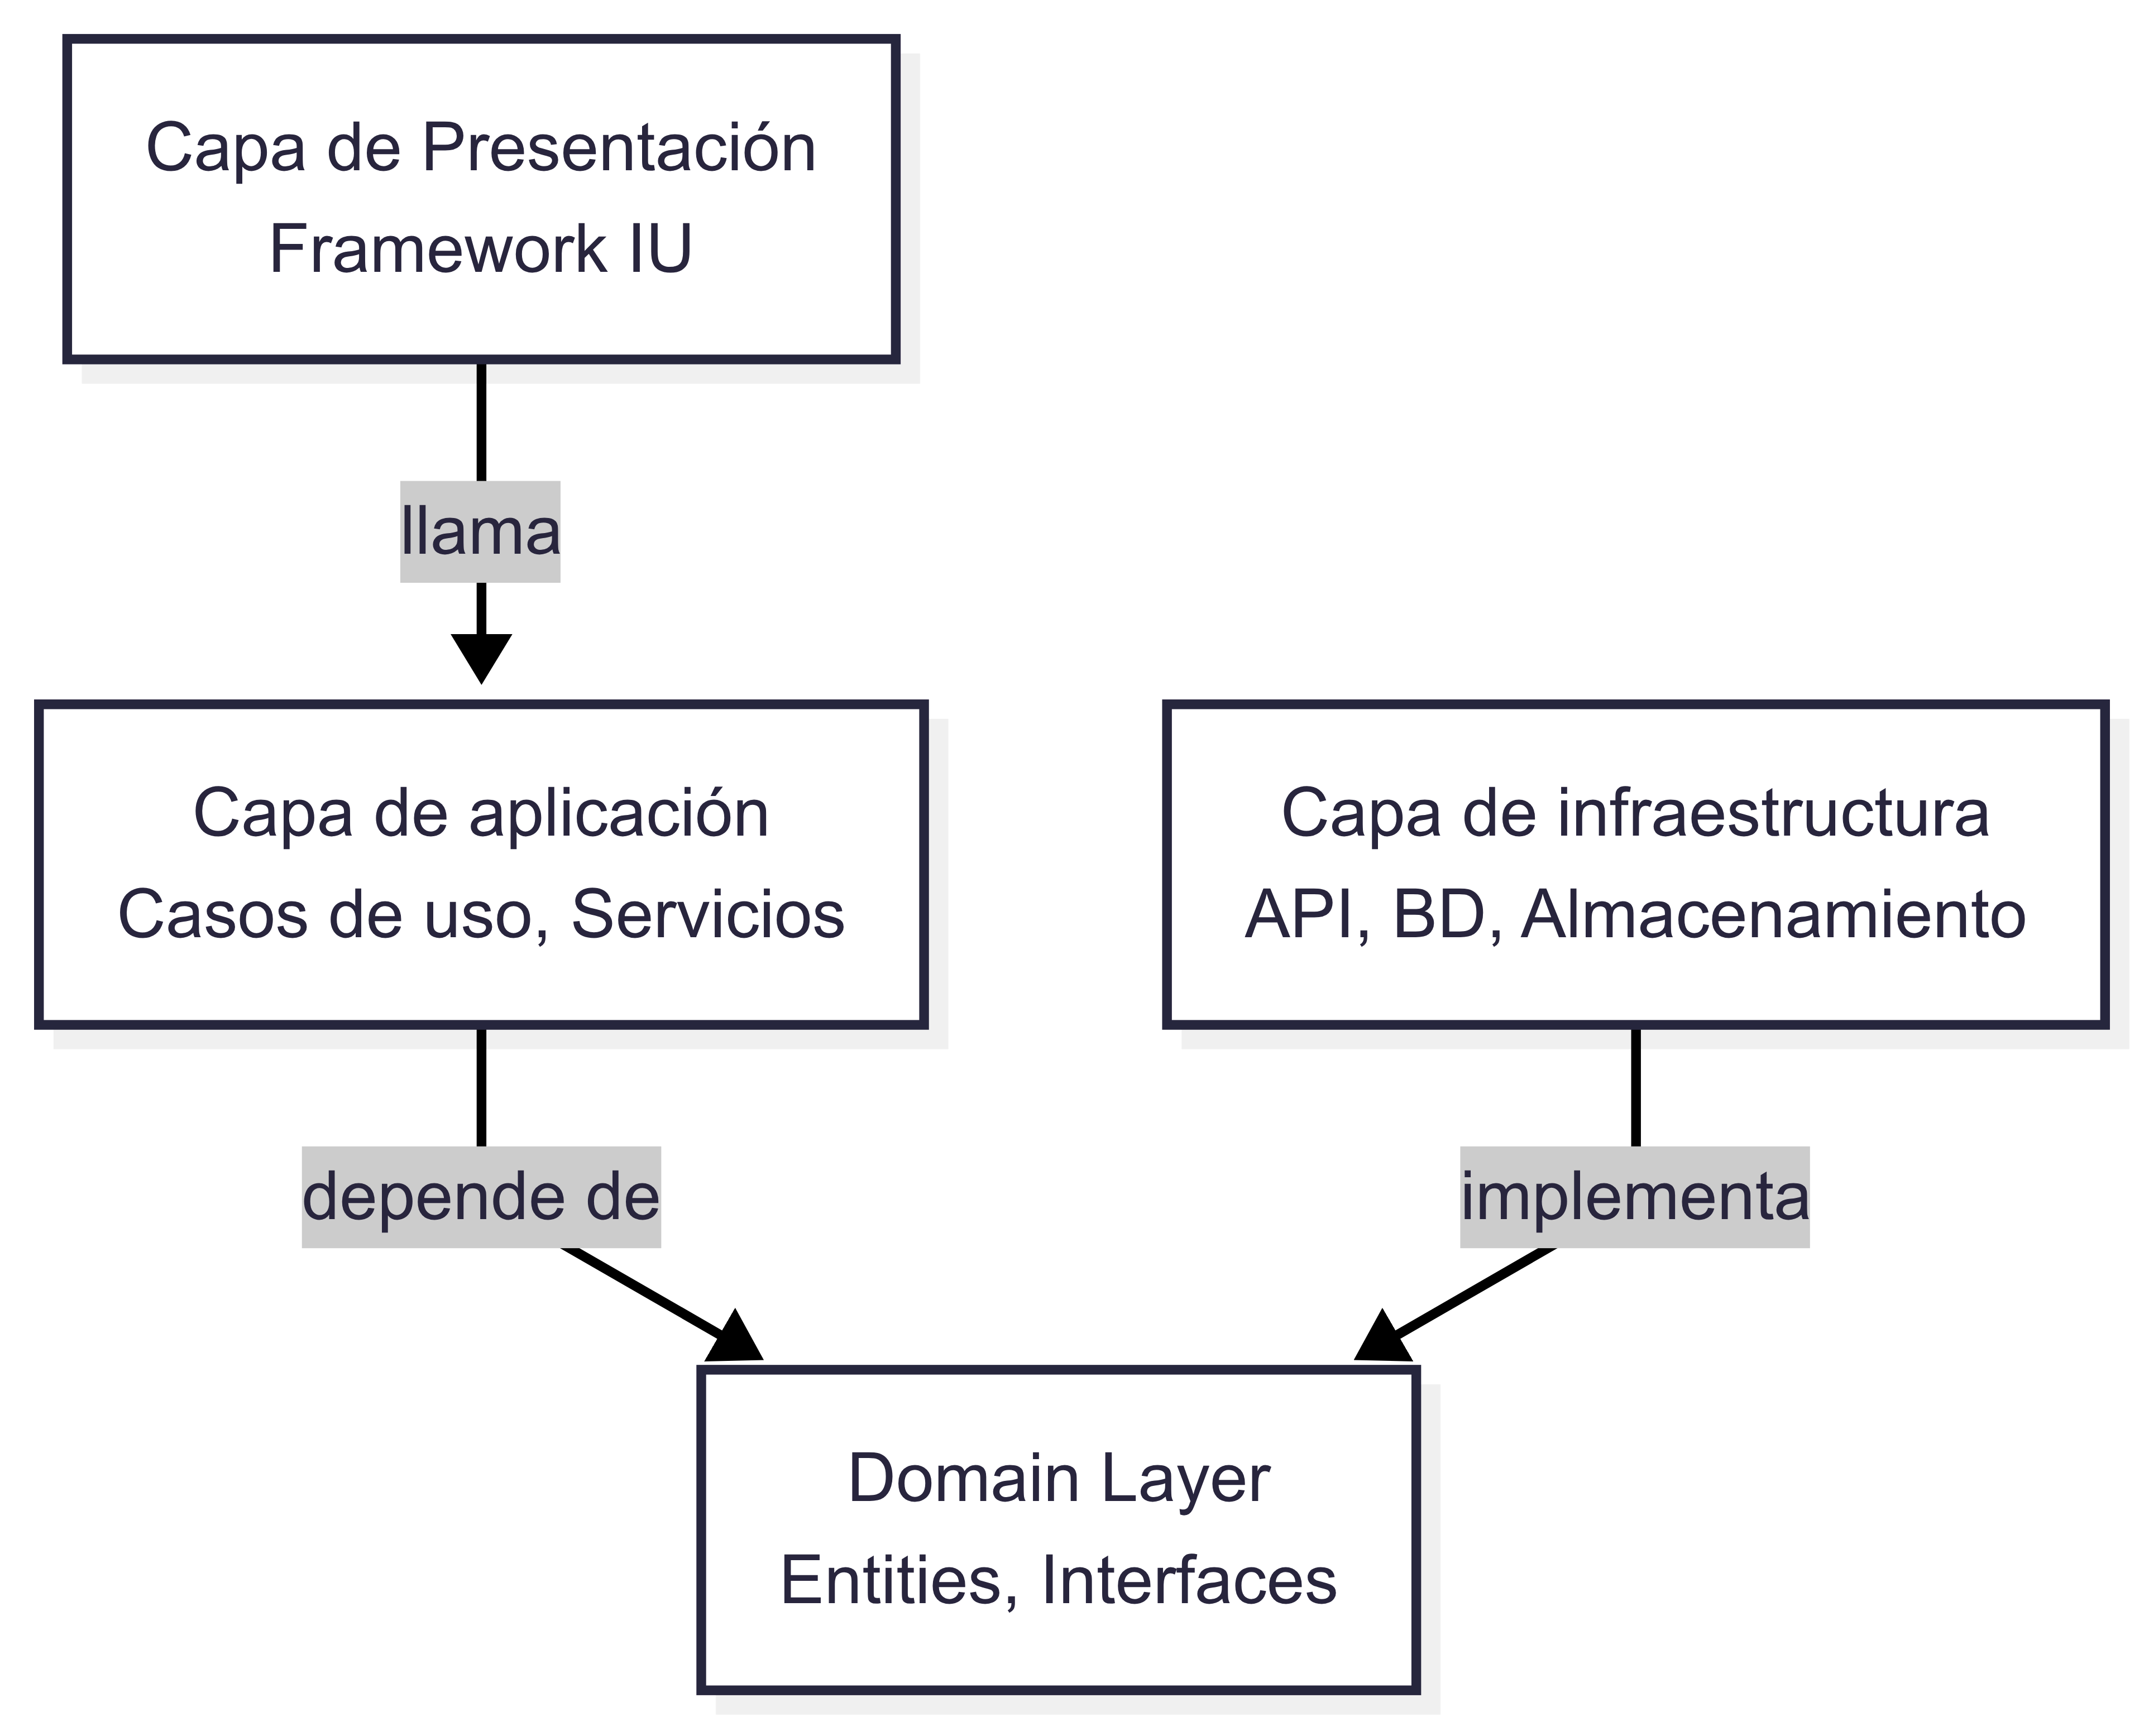
\includegraphics[width=0.8\textwidth]{assets/clean-architecture-mobile.png}
  \caption{Diagrama de arquitectura limpia en aplicación móvil.}
  \label{fig:clean-architecture-mobile}
\end{figure}

Las flechas representan cómo accede cada capa a las demás.
El acceso se hace de la capa más externa a la más interna, es decir, la capa de dominio (la más interna) no puede saber nada sobre las otras capas, pero la capa de presentación puede acceder a la capa de dominio y a la capa de aplicación.

La capa de aplicación no utiliza directamente la capa de infraestructura, sino que lo hace a través de interfaces definidas en la capa de dominio. La capa de infraestructura se encarga de implementar estas interfaces, lo que permite cambiar la implementación de la capa de infraestructura sin afectar a la capa de dominio, de aplicación ni la de presentación.

De esta manera se consigue una separación de responsabilidades y una independencia de la infraestructura, lo que permite cambiar la implementación de cualquier capa sin afectar al resto del sistema.
También permite hacer pruebas unitarias e integración de manera más sencilla, ya que permite \gls{mockear} las interfaces de la capa de infraestructura y probar la lógica de negocio sin necesidad de depender de la implementación concreta de la capa de infraestructura.

\subsection{Desarrollo de artefactos del primer sprint}
Tal y como se ha definido en la \hyperref[sec:metodologia]{sección de metodología}, cada sprint se va a enfocar en una parte del proyecto. En este caso, el primer sprint se va a centrar en historias de usuario del servidor solamente. El segundo sprint se centrará en las historias de usuario del cliente móvil y una vez analizado el estado de ambos productos, se decidirá si comenzar a tener sprints conjuntos.

En la metodología Scrum se seleccionan historias de usuario hasta que la suma de las estimaciones de las historias de usuario sea menor o igual a la velocidad del equipo para ese sprint.
La velocidad del equipo se define como la cantidad de puntos de historia que el equipo puede completar en un sprint, y se calcula a partir de los sprints anteriores.
En este caso, como es el primer sprint y no hay una velocidad definida, se escogen historias de usuario fijándose en el tipo de tarea e intentando no tener una suma de puntos de historia muy alta.

Una vez se termina el sprint, en el proceso de retrospectiva se analiza cuántas historias de usuario se han completado o cuantas se han quedado a medias, y se ajusta la velocidad del equipo para el siguiente sprint. Este proceso se repite en cada sprint hasta que el equipo tiene una velocidad estable y se puede obtener una estimación más precisa de cuántas historias de usuario pueden completarse en cada sprint.

Durante la especificación del sprint backlog se va a estudiar si hay historias de usuario que puedan ser divididas en distintas historias y una vez se hayan definido las historias de usuario que se van a implementar en el sprint, se definirán las tareas correspondientes a cada historia de usuario junto con su estimación en horas.
En el momento que se disponga de estimaciones en horas de tareas, es posible realizar un diagrama de Gantt para el sprint con las tareas y su duración estimada.

\subsection{Planificación de entregas}
En esta sección se va a definir los objetivos generales que tendremos para cada entrega en caga sprint. Estos objetivos son estimados y pueden variar dependiendo de la velocidad real del equipo, puede ser que se consiga más en un sprint o menos. Esta planificación se realiza para que, en el caso de que tuviéramos un cliente, se le pudiera dar una estimación del producto que va a ir recibiendo en cada entrega.

En este caso y en este tipo de proyecto, sirve para tener un enfoque claro de lo que se quiere conseguir en cada sprint y no desviarse realizando otras tareas.
Definir qué se va a entregar en cada sprint también ayudará priorizar qué historias de usuario se van a realizar en cada sprint.

Teniendo en cuenta que el desarrollo del proyecto comienza la última semana de junio de 2025, que cada sprint dura dos semanas y que la fecha límite de entrega del proyecto es el 5 de septiembre de 2025, se presentan un total de 11 semanas para el proyecto. Teniendo en cuenta que el sprint 0 tiene una duración de una semana, se definen un total de 5 sprints para el desarrollo del proyecto.

Los objetivos de cada sprint quedarían de la siguiente manera:
\begin{itemize}
    \item \textbf{Sprint 1}: Implementación de la API REST del servidor, incluyendo la gestión de usuarios, autenticación y autorización. Durante esta iteración se busca implementar una gestión de usuarios simple junto con toda la estructura base del proyecto.
    \item \textbf{Sprint 2}: Implementación de la aplicación móvil. Definición e implementación de módulos nativos para el acceso a archivos multimedia y permisos. Durante esta iteración se busca implementar una aplicación de gestión de galería básica sin funcionalidades de sincronización.
    \item \textbf{Sprint 3}: Implementación de todo el procesado multimedia en el servidor: generación de miniaturas, subida y compresión de imágenes y vídeos, etiquetado basado en metadatos, etc. En el cliente se implementará la subida de archivos multimedia a el servidor y la visualización de los archivos subidos.
    \item \textbf{Sprint 4}: Implementación de la sincronización automática de archivos multimedia en el cliente móvil tanto como la visualización del estado de la galería en el servidor. En esta iteración se implementará principalmente toda la conexión automática entre el cliente y el servidor, así como la sincronización de archivos multimedia.
    \item \textbf{Sprint 5}: Implementación de la gestión de usuarios desde el cliente móvil, incluyendo la gestión de permisos en las galerías, álbumes y archivos. Durante esta última iteración se implementará el uso compartido de galerías y álbumes entre usuarios.
    \item \textbf{Sprint 6}: Implementación de interfaz de usuario para gestión de configuración del servidor. Implementación de servicio de almacenamiento de archivos multimedia nativo en el servidor.
\end{itemize}
Este último sprint, aunque no entra en el plazo de entrega del proyecto, se define para tener una idea de lo que se quiere conseguir en el futuro, poder tener una planificación más clara de lo que se quiere conseguir en el proyecto y facilitar contribuciones al proyecto open-source.

Tal y como se ha mencionado anteriormente, estos objetivos son estimados y por la naturaleza de la metodología Scrum pueden ir variando a lo largo del desarrollo. Al final de cada sprint se realizará una retrospectiva donde se ajustarán los backlogs y objetivos de los siguientes sprints en función de lo que se haya conseguido en el sprint anterior.

\section{Tecnologías}
Una vez realizado el análisis de las distintas tecnologías que se pueden utilizar para el desarrollo del proyecto en el capítulo \ref{sec:tecnologias} y definidos los objetivos principales del proyecto (sección \ref{sec:objetivos}), se ha decidido utilizar las siguientes tecnologías para cada parte del proyecto:

\subsection{Servidor}
Para el servidor, cualquiera de las dos soluciones sería completamente válida. Go podría ser la mejor opción por su enfoque en la simplicidad y la facilidad de uso, especialmente para aplicaciones web y servicios de red. Sin embargo, Rust ofrece ventajas significativas en términos de seguridad de memoria y rendimiento, lo que lo convierte en una opción atractiva para aplicaciones que requieren alta concurrencia y eficiencia.

En este proyecto se busca alto rendimiento, seguridad, facilidad de contribuir al proyecto y un lenguaje sólido que no sea propenso a fallos.
Es por esto que Rust es la mejor opción para este caso. \parencite{rust-for-safety-and-performance}

Tal como se ha comentado anteriormente, Rust facilita la seguridad en la ejecución del código gracias a su estricto compilador.
Ofrece una gran variedad de funcionalidades sin coste en rendimiento junto con su sistema de propiedad y préstamos que permite gestionar la memoria de forma segura y eficiente, evitando errores comunes como las condiciones de carrera o los punteros nulos sin necesidad de un recolector de basura (\acrfull{gb}).

Aunque la curva de aprendizaje de Rust es más pronunciada, los beneficios a largo plazo en términos de seguridad y rendimiento justifican esta inversión inicial.

Invertir en aprender este lenguaje no solo favorecerá el desarrollo de este proyecto, sino que también proporcionará habilidades valiosas para futuros proyectos en el ámbito del desarrollo de software, el cual al final es uno de los objetivos de hacer un proyecto de este tamaño.

El trabajo con tecnologías y paradigmas de programación poco familiares para el equipo contribuye al desarrollo de nuevas competencias y a la ampliación del conocimiento en el ámbito del desarrollo de software, lo cual resulta fundamental para el crecimiento profesional.

Para la parte de servidor se va a hacer uso de uno de los lenguajes más venerados en la actualidad en el mundo de la programación: \textbf{Rust}.

Rust es un lenguaje de programación de sistemas que se centra en la seguridad, el rendimiento y la concurrencia. Se ha convertido en una opción popular para el desarrollo de aplicaciones de alto rendimiento y sistemas críticos.
Aunque Rust es un lenguaje de bajo nivel, su sintaxis es muy similar a la de otros lenguajes de programación como C++ o Java, lo que facilita su aprendizaje para los programadores que ya tienen experiencia en estos lenguajes, permitiendo un desarrollo más seguro, rápido y eficiente.

\begin{itemize}
    \item \textbf{Rendimiento}: es conocido por su alto rendimiento, lo que lo convierte en una excelente opción para aplicaciones que requieren un procesamiento intensivo de datos. Aunque es un lenguaje enfocado a sistemas, el rendimiento de sus librerías para desarrollo web es muy bueno, como se puede ver en distintos benchmark \parencite{rust-benchmark}.
    \item \textbf{Seguridad}: tiene un sistema de tipos y un modelo de propiedad que ayudan a prevenir errores comunes de programación, como desbordamientos de búfer y condiciones de carrera.
    \item \textbf{Concurrencia}: soporta de manera nativa y sencilla la escritura de código concurrente y paralelo, lo que es esencial para aplicaciones que manejan múltiples tareas al mismo tiempo.
        Gracias a su implementación de \gls{fearless-concurrency}, Rust permite a los desarrolladores escribir código concurrente sin preocuparse por errores comunes como condiciones de carrera o deadlocks, lo que facilita la creación de aplicaciones altamente eficientes y escalables.
    \item \textbf{Manejo de errores}: tiene un enfoque único para el manejo de errores, utilizando tipos de datos como \texttt{Result} y \texttt{Option} para representar resultados exitosos y fallidos, lo que ayuda a evitar errores en tiempo de ejecución, consiguiendo de esta manera no encontrarnos con errores inesperados a la hora de ejecutar la aplicación.
    \item \textbf{Ecosistema}: cuenta con un ecosistema en crecimiento, con una amplia variedad de bibliotecas y herramientas que facilitan el desarrollo de aplicaciones.
\end{itemize}


Para el desarrollo de el servidor de sincronización se ha decidido usar del framework de aplicaciones web \href{https://github.com/tokio-rs/axum?tab=readme-ov-file}{\textbf{Axum}}.
Axum es un framework de aplicaciones web construido sobre Tokio, una biblioteca de programación asíncrona para Rust. Axum se centra en la simplicidad y la facilidad de uso, lo que lo convierte en una excelente opción para desarrollar aplicaciones web rápidas y eficientes.
Aunque hay varios frameworks más eficientes en términos de velocidad a la hora de realizar benchmarks\footnote{\href{https://web-frameworks-benchmark.netlify.app/result?l=rust}{Comparativa frameworks de Rust}} \footnote{\href{https://www.techempower.com/benchmarks/\#section=data-r21&test=composite&hw=ph}{Comparativa con frameworks de otros lenguajes}}, algunos de ellos tienen un tiempo de compilación demasiado alto, por lo que puede llegar a hacer más lento el desarrollo.
Además, ninguno de los demás frameworks de Rust tiene una comunidad tan activa como la de Axum ni una documentación tan completa.

Axum al estar desarrollado sobre la librería de Tokio\footnote{Librería de Rust más usada para la programación asíncrona}, garantiza un soporte a largo plazo que otros frameworks no garantizan. Además, es \href{https://lib.rs/crates/axum}{la librería más descargada }mensualmente para aplicaciones web en Rust.

Como se puede ver en los benchmark hay frameworks de otros lenguajes que pueden parecer más sencillos que Rust y que ofrecen el mismo o mejor rendimiento, pero como se ha comentado anteriormente, el punto principal de Rust no es únicamente su rendimiento, sino la seguridad que proporciona el propio lenguaje y lo poco propenso que es a errores en tiempo de compilación, lo que hace que la aplicación sea mucho más robusta, segura y sostenible a largo plazo.


\subsection{Móvil}
Para el desarrollo de la aplicación móvil se ha optado por el nuevo framework de desarrollo multiplataforma, \textbf{Lynx.js}.

Esta es una opción muy arriesgada para este proyecto ya que es un framework que aún está en desarrollo y no tiene una comunidad tan grande como otros frameworks más consolidados como React Native o Flutter.

Trabajar con un framework que aún está en desarrollo y que tiene muchas funcionalidades por implementar puede parecer arriesgado, pero también ofrece la oportunidad de contribuir al desarrollo del framework y ayudar a mejorar la herramienta para el futuro.
El hecho de que no haya un punto de partida tan avanzado como en otros frameworks hará que el equipo tenga que enfrentarse a retos y problemas que no se han resuelto aún, lo que puede ser una gran oportunidad para aprender y mejorar las habilidades de desarrollo.
Desarrollar ese tipo de funcionalidades en un framework conseguirá que el equipo tenga un conocimiento más profundo de cómo funciona el framework y cómo se pueden implementar soluciones eficientes y efectivas.

Lynx.js es un framework inspirado en React Native. El desarrollo de la aplicación se hace con React el cual se compila a código nativo de la plataforma. El framework soporta componentes de cualquier framework de desarrollo web, aunque está pensado para usar React con componentes definidos por el framework de desarrollo.

Aunque pueda parecer igual que React Native, Lynx añade algunas cosas que le faltan a React Native. Uno de los mayores problemas de React Native es su rendimiento en algunas situaciones, ya que este solamente hace uso de un solo hilo de ejecución, lo cual no permite una buena gestión de las tareas. Por ejemplo, no puede obtener datos de una API mientras que se actualiza lo que se muestra al usuario.

Sin embargo, Lynx tiene se ejecuta sobre dos hilos, un hilo principal y un hilo secundario.
Gracias a esto, es posible especificar en qué hilo se va a ejecutar cada función, consiguiendo de esta manera que tareas como mostrar rápidamente la interfaz se hagan lo más rápido posible mientras que en el hilo secundario se obtienen los datos de la API.
Esto da una experiencia al usuario mucho más fluida y rápida, principalmente gracias a el \gls{ifr} (\acrshort{ifracr}).

Para conseguir esto, Lynx altera el ciclo de vida de los componentes de React (figura \ref{fig:lynx-component-lifecycle}), consiguiendo deshacerse de cuellos de botella típicos que aparecen en los frameworks de desarrollo móvil asegurando un rendimiento óptimo y una experiencia de usuario fluida.

\begin{figure}[h]
    \begin{center}
        \includegraphics[width=\textwidth]{lynx-lifecycle.png}
    \end{center}
    \caption{Ciclo de vida de los componentes en Lynx.js (\href{https://lynxjs.org/react/lifecycle.html}{Documentación})}
    \label{fig:lynx-component-lifecycle}
\end{figure}


Dado que la aplicación necesitará hacer uso de módulos nativos de los teléfonos, será necesario implementarlos para cada plataforma.
Esto se puede hacer de manera sencilla, ya que el framework permite la creación de módulos nativos los cuales se pueden llamar desde el código escrito con React.

Este es uno de los puntos fuertes de la aplicación, ya que permitirá programar haciendo uso de React, el cual es un framework muy conocido y utilizado, pero a la vez permite usar módulos nativos de cada plataforma, lo que da una gran flexibilidad a la hora de desarrollar la aplicación de forma nativa en todas las plataformas.

Lynx usa una aplicación nativa \textit{Lynx Explorer}, con la cual se puede visualizar el estado de la aplicación conforme se va desarrollando en tiempo real.
Esta aplicación se encarga de ejecutar el código compilado de Lynx.js y permite debuggear la aplicación gracias a su \href{https://github.com/lynx-family/lynx-devtool}{herramienta de depuración}.
Para poder hacer uso de los módulos nativos es necesario implementarlos en el Explorer, un proyecto que implementa el runtime que utiliza Lynx.js por debajo tanto en Android como iOS, compilar el código del mismo y una vez se ha compilado la aplicación con nuestro módulo nativo, se puede llamar a la implementación nativa desde la aplicación escrita en Lynx.js.

A la hora de compilar la aplicación para ser usada en producción, Lynx se incorpora sobre un SDK de Android o iOS. Gracias a esto se puede incorporar la aplicación en cualquier otra aplicación existente con tan solo compilar el código y añadirlo con el SDK de Lynx en la plataforma que se desee.
En este caso se usará una estructura de aplicación que proporcionan en \href{https://github.com/lynx-family/integrating-lynx-demo-projects}{su repositorio oficial de proyectos de ejemplo}, los cuales contienen proyectos vacíos que hacen uso de el SDK correspondiente en cada plataforma, por lo que tan solo será necesario incorporar la aplicación hecha con Lynx.js compilada y compilar el proyecto para cada plataforma.

El proceso de compilación de una aplicación para producción sigue siendo complejo aún, ya que tal y como se ha comentado, Lynx.js no tiene aún una manera definitiva de compilar un proyecto sin tener que integrarlo mediante el SDK de Lynx en un proyecto nativo de Android o iOS. Aún así, el repositorio con los proyectos de ejemplo proporciona una buena base para empezar a trabajar con Lynx.js y permite el desarrollo de la aplicación sin tener que preocuparnos por la configuración del proyecto.

Todo esto, junto con los comandos y repositorios necesarios viene detallado en el artículo hecho por el equipo de Lynx \parencite{lynx-native-modules}.

Dado que para el desarrollo de aplicaciones en iOS es necesario tener un sistema de Apple, este proyecto se centrará únicamente en la aplicación para Android, aunque el código de la aplicación será el mismo para ambas plataformas a diferencia de la implementación de los módulos nativos, que serán diferentes para cada plataforma.

En resumen, las ventajas de usar este framework con respecto a otros son:
\begin{itemize}
    \item \textbf{Rendimiento}: al compilar a código nativo, el rendimiento es mucho mejor que el de otros frameworks como Flutter. Además, Lynx ofrece una tecnología de doble hilo, haciendo que la aplicación sea mucho más fluida y rápida en comparación con otras tecnologías.
    \item \textbf{Flexibilidad}: permite la creación de módulos nativos para cada plataforma, lo que da una gran flexibilidad a la hora de desarrollar la aplicación.
    \item \textbf{Simplicidad}: la sintaxis es muy similar a la de React, lo que facilita su aprendizaje para los programadores que ya tienen experiencia en este framework.
    \item \textbf{Documentación}: la documentación es muy completa y está en constante actualización.
\end{itemize}

¿Por qué no se ha optado por otras opciones como Flutter o Kotlin Multiplatform?
\begin{itemize}
    \item \textbf{Flutter}: aunque es un framework muy potente y con una comunidad muy activa, su rendimiento no es tan bueno como el de Lynx.js.
        Flutter renderiza un ``canvas'' que utiliza un motor gráfico que se asemeja a un motor para juegos para renderizar la interfaz de usuario, haciendo que la experiencia de usuario no sea tan fluida como podría ser la de otro framework.
    \item \textbf{Kotlin Multiplatform}: aunque es una opción interesante, la comunidad y la documentación son mucho más limitadas que las de Lynx.js. La curva de aprendizaje es mucho más pronunciada, ya que se utiliza Kotlin junto con una gran cantidad de librerías las cuales necesitan de un estudio profundo para su uso.

        Aportaría el mejor rendimiento sin tener que programar la aplicación de forma nativa para todos los dispositivos (los dispositivos comparten código pero hay que implementar la mayoría de forma nativa para las distintas plataformas), pero el desarrollo sería mucho más lento y tedioso, lo cual además complicaría la aportación al proyecto Open Source.
    \item \textbf{React Native}: aunque es un framework muy conocido y utilizado, su rendimiento no es tan bueno como el de Lynx.js.
        Es una opción muy parecida a Lynx.js, pero a largo plazo la aplicación podría verse afectada por el rendimiento.
        Dada la similitud con Lynx.js y las ventajas que ofrece, se ha optado por este último.
\end{itemize}

Este framework ha sido desarrollado de cero por el equipo de TikTok. Es utilizado por ellos para el desarrollo de varias de sus aplicaciones, por lo que aunque ha cambiado a ser Open-Source hace poco con su versión 3.2.0. Es un framework que ya ha sido probado en producción en aplicaciones como \textbf{TikTok Studio}, \textbf{Disney100 en TikTok}, \textbf{The Met Gala en TikTok} tal y como comentan en el artículo en el que anunciaron que Lynx.js pasaba a ser Open-Source \parencite{lynx-article}.

\subsection{Inicialización del entorno de desarrollo}
En esta sección se va a detallar cómo se ha procedido a la inicialización del entorno de desarrollo tanto para el servidor como para la aplicación móvil.
\paragraph{Servidor}
\subparagraph{}
Para la inicialización del entorno de desarrollo del servidor se ha tomado como referencia la estructura de ejemplo que se puede encontrar en el artículo consultado sobre la arquitectura hexagonal en Rust \parencite{rust-hexagonal-architecture}. Éste quedaría de la siguiente manera:
\dirtree{%
.1 /.
.2 migrations/.
.3 20240603122606\_create\_authors.down.sql.
.3 20240603122606\_create\_authors.up.sql.
.2 src/.
.3 bin/.
.4 server/.
.5 main.rs.
.3 lib/.
.4 domain/.
.5 blog/.
.6 models/.
.7 author.rs.
.6 models.rs.
.6 ports.rs.
.6 service.rs.
.5 blog.rs.
.4 inbound/.
.5 http/.
.6 handlers/.
.7 create\_author.rs.
.6 handlers.rs.
.6 responses.rs.
.5 http.rs.
.4 outbound/.
.5 email\_client.rs.
.5 prometheus.rs.
.5 sqlite.rs.
.4 config.rs.
.4 domain.rs.
.4 inbound.rs.
.4 lib.rs.
.4 outbound.rs.
.2 .env.template.
.2 .gitignore.
.2 Cargo.lock.
.2 Cargo.toml.
.2 LICENSE.
.2 README.md.
}

Se define la siguiente estructura:
\begin{itemize}
    \item \textbf{migrations}: esta carpeta contiene los archivos de migración de la base de datos, que se utilizan para crear y actualizar la estructura de la base de datos. En este caso, contiene un archivo para crear la tabla de autores. Esta carpeta contiene todos los archivos necesarios para inicializar la base de datos y para borrarla si es necesario.
    \item \textbf{src}: esta carpeta contiene todo el código fuente del servidor, con las siguientes subcarpetas:
        \begin{itemize}
            \item \textbf{bin}: contiene el código que se ejecuta al iniciar el servidor, el punto de entrada de la aplicación. En esta carpeta no hay ningún tipo de lógica implementada, tan solo se inicializa el servidor, se definen las implementaciones de las interfaces y se inicia el servidor con las dependencias que necesite.
            \item \textbf{lib}: esta carpeta contiene todo el código de la aplicación, dividido siguiendo una filosofía hexagonal de la siguiente manera:
                \begin{itemize}
                    \item \textbf{domain}: contiene el código del dominio de la aplicación, es decir, la lógica de negocio. Se definen los modelos, puertos (interfaces) y servicios que se utilizan en la aplicación.
                    \item \textbf{inbound}: contiene el código de la capa de entrada de la aplicación, es decir, las interfaces que se exponen al exterior. En este caso, contiene un módulo HTTP que define los handlers (controladores) que se encargan de recibir las peticiones HTTP y devolver las respuestas correspondientes.
                    \item \textbf{outbound}: contiene el código de la capa de salida de la aplicación, es decir, las implementaciones de las interfaces que se utilizan en la capa de dominio. En este caso, contiene un cliente de correo electrónico, un cliente de Prometheus y un cliente SQLite que se encargan de enviar correos electrónicos, exponer métricas y acceder a la base de datos respectivamente.
                    \item \textbf{config.rs}: contiene la configuración de la aplicación, como las variables de entorno y los parámetros de configuración.
                    \item Los demás archivos definen los módulos de Rust.
                \end{itemize}
        \end{itemize}
\end{itemize}

Además de esos archivos, existen los archivos típicos de un proyecto de Rust, como son el \texttt{Cargo.toml} y el \texttt{Cargo.lock}, que definen las dependencias del proyecto y la versión de las mismas, así como el archivo \texttt{README.md} que contiene la documentación del proyecto y el archivo \texttt{LICENSE} que contiene la licencia del proyecto. Tanto el archivo \texttt{README.md} como el \texttt{LICENSE} se han redactado en inglés al igual que todo el código, puesto que el proyecto está pensado para ser Open-Source y se busca que cualquier persona pueda entenderlo y contribuir al mismo.

En este proyecto, tal y como se ha definido anteriormente, se utiliza un enfoque de arquitectura monolítica modular siguiendo el patrón de código \acrshort{cqrs}.
En este enfoque, los archivos van a estar organizados en módulos en vez de agrupados por capas, lo que permite definir de una manera más clara y flexible las funcionalidades de cada módulo.
Además, en la capa de aplicación se separan los casos de uso en comandos y consultas (las consultas son las que se encargan de obtener datos y los comandos son los que se encargan de modificar el estado del sistema), lo que permite tener una mejor organización del código y una mayor flexibilidad a la hora de añadir nuevas funcionalidades.

Este es un enfoque común en aplicaciones web modernas, ya que gracias a esto se puede conseguir funcionalidades como añadir caché a las consultas, realizar pruebas unitarias de los comandos y consultas de manera independiente, y tener una mejor organización del código en general.

Si se adaptara este proyecto de ejemplo a la estructura que se utilizará, la estructura sería de la siguiente manera:

\newpage
\dirtree{%
.1 /.
.2 migrations/.
.3 20240603122606\_create\_authors.down.sql.
.3 20240603122606\_create\_authors.up.sql.
.2 src/.
.3 bin/.
.4 server/.
.5 main.rs.
.3 lib/.
.4 blog/.
.5 domain/.
.6 models.rs.
.6 models/.
.7 author.rs.
.6 ports.rs.
.5 application/.
.6 commands/.
.7 create\_author.rs.
.6 queries/.
.7 get\_authors.rs.
.5 infrastructure/.
.6 sqlite.rs.
.6 email\_client.rs.
.5 interface/.
.6 http/.
.7 handlers.rs.
.7 handlers/.
.8 create\_author.rs.
.7 responses.rs.
.4 monitoring/.
.5 infrastructure/.
.6 prometheus.rs.
.4 shared/.
.5 config.rs.
.5 lib.rs.
.2 .env.template.
.2 .gitignore.
.2 Cargo.lock.
.2 Cargo.toml.
.2 LICENSE.
.2 README.md.
}

\paragraph{Cliente móvil}
\subparagraph{}
Siguiendo la arquitectura limpia para una aplicación móvil, definida en la Figura \ref{fig:clean-architecture-mobile}, la estructura del cliente móvil es muy similar a la del servidor, pero con algunas diferencias.

En este caso no se utiliza el patrón de código \acrshort{cqrs}, ya que no es necesario en una aplicación móvil, pero sí se sigue una estructura modular similar a la del servidor, donde cada módulo tiene una responsabilidad clara y bien definida.
La única adición que se presenta con respecto a la estructura del servidor es que en la aplicación móvil existe una capa de presentación que se encarga de la interfaz de usuario y de la interacción con el usuario, la cual sería la equivalente a la capa de interface que se definió en el servidor para la comunicación con el exterior (en el caso del servidor, mediante comunicación HTTP).

Una estructura de ejemplo para una aplicación móvil podría ser la siguiente:

\dirtree{%
.1 mobile-app/.
.2 src/.
.3 modules/.
.4 blog/.
.5 domain/.
.5 application/.
.6 services/.
.7 authorService.ts.
.7 blogService.ts.
.5 infrastructure/.
.5 presentation/.
.4 monitoring/.
.5 application/.
.6 services/.
.7 monitoringService.ts.
.5 infrastructure/.
.5 presentation/.
.4 shared/.
.5 config/.
.5 application/.
.6 services/.
.7 httpService.ts.
.7 storageService.ts.
.5 infrastructure/.
.5 presentation/.
.5 types/.
.3 navigation/.
.3 App.tsx.
.2 assets/.
.2 \_\_tests\_\_/.
.2 archivos de configuración del proyecto...
}

La principal diferencia que hay con respecto al servidor es que en la capa de aplicación no se seguirá un patrón CQRS y se implementarán servicios que se encargan de toda la lógica.
Además, la capa de interfaz se cambia por una capa de presentación, que se encargará de la interfaz de usuario y de la interacción con el usuario.

Para la inicialización del entorno de desarrollo del cliente móvil, además del directorio que implementa la aplicación usando Lynx.js se necesitará un directorio para el código de Lynx Explorer, puesto que se realizará una implementación de módulos nativos para acceder a funcionalidades como el acceso a imágenes en el dispositivo tanto como para gestionar los permisos necesarios de la aplicación.
Toda la documentación que se ha utilizado para inicializar el directorio de Lynx Explorer se puede encontrar en la \href{https://lynxjs.org/guide/use-native-modules.html#platform=android}{documentación oficial de Lynx.js} sobre implementación de módulos nativos.


\section{Sprint 1}
Tal y como se ha definido en la sección \ref{sec:planificacion-inicial}, el primer sprint se centra en la base de nuestra aplicación web, desarrollando la estructura inicial del servidor, gestión de usuarios y subida y descarga sencilla de archivos.
Para ello, se han elegido las historias de usuario relacionadas con el objetivo de este sprint y se han desarrollado definiendo sub-historias de usuario si fueran necesarias, criterios de aceptación y las tareas necesarias para su implementación.

Las historias de usuario se han seleccionado de manera aproximada, puesto que al ser el primer sprint no tenemos una velocidad de equipo definida. Existe la posibilidad de que algunas historias de usuario no se completen en este sprint o de que se completen más de las previstas, por lo que se ha dejado un margen de maniobra para que el equipo pueda adaptarse a la realidad del desarrollo.

Cuando se termine el sprint, se calculará la velocidad del equipo la cual se utilizará para planificar los siguientes sprints, de manera que se pueda ajustar la cantidad de historias de usuario a desarrollar en cada uno de ellos.

Una vez definidas todas las tareas que se van a realizar en este sprint, se ha realizado un diagrama de Gantt para planificar el tiempo que se va a dedicar a cada una de ellas, teniendo en cuenta que el sprint tiene una duración de dos semanas, y se dará un orden de prioridad a las tareas que se consideren más importantes para llegar a el objetivo del sprint.

% TODO: Move this to an appendix at the end of the document, alongside the product backlog and other sprints.
\subsection{Historias de usuario}
En esta sección se detallan las historias de usuario y técnicas que se han elegido para este sprint. Se va a hacer una breve descripción de cada una de ellas, así como los criterios de aceptación y las tareas necesarias para su implementación. Si fuera necesario, se definirán sub-historias de usuario para facilitar su desarrollo.

Las seleccionadas son las siguientes:
\begin{itemize}
    \item HU05: Inicio de sesión - 5 PH
    \item HU06: Cerrar sesión - 2 PH
    \item HU13: Crear cuentas - 8 PH
    \item HT03 API REST en Rust - 13 PH
    \item HT05: Autenticación JWT - 5 PH
    \item HT08: Base de datos - 8 PH
    \item HT18.1: Binario - 2 PH
    \item HT19: Dockerización - 3 PH
    \item HT20.1: Documentación del proyecto en GitHub - 5 PH
    \item HT20.2: Documentación de la API REST con OpenAPI - 5 PH
\end{itemize}

Estas historias de usuario y técnicas suman un total de 56 puntos de historia (PH). Es importante destacar que la estimación en puntos de historia representa la complejidad relativa de cada historia, mientras que las tareas de desarrollo se estiman en horas de trabajo efectivo.

\subsection{Descomposición en tareas de desarrollo}

% HU05: Inicio de sesión
\begin{table}[H]
    \begin{center}
        \begin{tabularx}{\textwidth}{|l|X|l|}
            \hline
            \textbf{Identificador HU05} & 
            \textbf{Como usuario, quiero iniciar sesión con contraseña o clave, para evitar que otros accedan a mis archivos} &
            \textbf{Estimación: 5 PH}\\
            \hline
            \multicolumn{3}{|p{\textwidth}|}{
                \begin{minipage}{\textwidth}
                    \centering
                    \vspace{0.5em}
                    \begin{tabular}{|l|p{8cm}|r|}
                        \hline
                        \textbf{Identificador} & \textbf{Título de la tarea de desarrollo} & \makecell{\textbf{Estimación}\\\textbf{(h)}} \\
                        \hline
                        Tarea 5-1U & Implementar endpoint para iniciar sesión & 2 \\
                        \hline
                        Tarea 5-2U & Validar credenciales de usuario contra la base de datos & 1.5 \\
                        \hline
                        Tarea 5-3U & Generar y devolver token JWT al usuario autenticado & 1.5 \\
                        \hline
                        Tarea 5-4U & Gestionar errores de autenticación (usuario no existe, contraseña incorrecta) & 1.5 \\
                        \hline
                        Tarea 5-5U & Documentar el endpoint de inicio de sesión en OpenAPI & 0.5 \\
                        \hline
                    \end{tabular}
                    \vspace{0.5em}
                \end{minipage}
            } \\
            \hline
            \multicolumn{3}{|p{\textwidth}|}{
                \textbf{Pruebas de aceptación:}
                    \begin{itemize}
                        \item El usuario puede iniciar sesión con su contraseña.
                        \item Cuando el usuario inicia sesión, se le devuelve un token JWT.
                        \item Si el usuario no existe, se devuelve un mensaje de error.
                        \item Si la contraseña o clave son incorrectas, se devuelve un mensaje de error.
                        \item El endpoint está documentado en OpenAPI.
                    \end{itemize}
            }\\
            \hline
            \multicolumn{3}{|p{\textwidth}|}{
                \textbf{Observaciones:}
                \begin{itemize}
                    \item El endpoint debe ser seguro (usar HTTPS).
                    \item El token JWT debe tener expiración configurable.
                \end{itemize}
            }\\
            \hline
        \end{tabularx}
    \end{center}
\end{table}

% HU06: Cerrar sesión
\begin{table}[H]
    \begin{center}
        \begin{tabularx}{\textwidth}{|l|X|l|}
            \hline
            \textbf{Identificador HU06} & 
            \textbf{Como usuario, quiero poder cerrar sesión en un dispositivo, para proteger mis datos si pierdo el móvil} &
            \textbf{Estimación: 2 PH}\\
            \hline
            \multicolumn{3}{|c|}{
                \begin{minipage}{\linewidth}
                    \centering
                    \vspace{0.5em}
                    \begin{tabular}{|l|p{8cm}|r|}
                        \hline
                        \textbf{Identificador} & \textbf{Título de la tarea de desarrollo} & \makecell{\textbf{Estimación}\\\textbf{(h)}} \\
                        \hline
                        Tarea 6-1 & Implementar endpoint para cerrar sesión (invalidar token JWT) & 1 \\
                        \hline
                        Tarea 6-2 & Gestionar lista negra de tokens JWT (opcional) & 1 \\
                        \hline
                    \end{tabular}
                    \vspace{0.5em}
                \end{minipage}
            } \\
            \hline
            \multicolumn{3}{|p{\textwidth}|}{
                \textbf{Pruebas de aceptación:}
                    \begin{itemize}
                        \item El usuario puede cerrar sesión y su token queda invalidado.
                        \item Tras cerrar sesión, el token no permite acceder a endpoints protegidos.
                    \end{itemize}
            }\\
            \hline
            \multicolumn{3}{|p{\textwidth}|}{
                \textbf{Observaciones:}
                \begin{itemize}
                    \item Si no se implementa lista negra, el token expira por tiempo.
                \end{itemize}
            }\\
            \hline
        \end{tabularx}
    \end{center}
\end{table}

% HU13: Crear cuentas
\begin{table}[H]
    \begin{center}
        \begin{tabularx}{\textwidth}{|l|X|l|}
            \hline
            \textbf{Identificador HU13} & 
            \textbf{Como administrador, quiero crear cuentas de usuario con permisos, para que varias personas puedan usar el servidor} &
            \textbf{Estimación: 8 PH}\\
            \hline
            \multicolumn{3}{|c|}{
                \begin{minipage}{\linewidth}
                    \centering
                    \vspace{0.5em}
                    \begin{tabular}{|l|p{8cm}|r|}
                        \hline
                        \textbf{Identificador} & \textbf{Título de la tarea de desarrollo} & \makecell{\textbf{Estimación}\\\textbf{(h)}} \\
                        \hline
                        Tarea 13-1 & Implementar endpoint para crear cuentas de usuario & 2 \\
                        \hline
                        Tarea 13-2 & Validar permisos de administrador para crear cuentas & 1.5 \\
                        \hline
                        Tarea 13-3 & Añadir roles/permisos a los usuarios & 1.5 \\
                        \hline
                        Tarea 13-4 & Gestionar almacenamiento seguro de contraseñas (hash) & 1.5 \\
                        \hline
                        Tarea 13-5 & Documentar el endpoint de creación de cuentas en OpenAPI & 0.5 \\
                        \hline
                        Tarea 13-6 & Pruebas unitarias de creación de usuario & 1 \\
                        \hline
                    \end{tabular}
                    \vspace{0.5em}
                \end{minipage}
            } \\
            \hline
            \multicolumn{3}{|p{\textwidth}|}{
                \textbf{Pruebas de aceptación:}
                    \begin{itemize}
                        \item Solo el administrador puede crear cuentas.
                        \item El usuario creado puede iniciar sesión.
                        \item Los roles/permisos se asignan correctamente.
                        \item El endpoint está documentado en OpenAPI.
                    \end{itemize}
            }\\
            \hline
            \multicolumn{3}{|p{\textwidth}|}{
                \textbf{Observaciones:}
                \begin{itemize}
                    \item Usar hash seguro para contraseñas (ej: Argon2).
                \end{itemize}
            }\\
            \hline
        \end{tabularx}
    \end{center}
\end{table}

% HT03: API REST en Rust
\begin{table}[H]
    \begin{center}
        \begin{tabularx}{\textwidth}{|l|X|l|}
            \hline
            \textbf{Identificador HT03} & 
            \textbf{Desarrollar API RESTful usando Rust y Axum} &
            \textbf{Estimación: 13 PH}\\
            \hline
            \multicolumn{3}{|c|}{
                \begin{minipage}{\linewidth}
                    \centering
                    \vspace{0.5em}
                    \begin{tabular}{|l|p{8cm}|r|}
                        \hline
                        \textbf{Identificador} & \textbf{Título de la tarea de desarrollo} & \makecell{\textbf{Estimación}\\\textbf{(h)}} \\
                        \hline
                        Tarea 3-1 & Crear estructura base del proyecto en Rust & 2 \\
                        \hline
                        Tarea 3-2 & Configurar Axum y dependencias principales & 2 \\
                        \hline
                        Tarea 3-3 & Definir rutas y controladores básicos & 2 \\
                        \hline
                        Tarea 3-4 & Implementar manejo de errores global & 2 \\
                        \hline
                        Tarea 3-5 & Añadir middlewares (logging, CORS, etc.) & 1.5 \\
                        \hline
                        Tarea 3-6 & Configurar variables de entorno y settings & 1.5 \\
                        \hline
                        Tarea 3-7 & Documentar endpoints iniciales & 1 \\
                        \hline
                        Tarea 3-8 & Pruebas de integración básicas & 1 \\
                        \hline
                    \end{tabular}
                    \vspace{0.5em}
                \end{minipage}
            } \\
            \hline
            \multicolumn{3}{|p{\textwidth}|}{
                \textbf{Pruebas de aceptación:}
                    \begin{itemize}
                        \item El servidor arranca y responde a peticiones básicas.
                        \item Los endpoints definidos funcionan correctamente.
                        \item El manejo de errores es consistente.
                    \end{itemize}
            }\\
            \hline
            \multicolumn{3}{|p{\textwidth}|}{
                \textbf{Observaciones:}
                \begin{itemize}
                    \item Seguir estructura modular y buenas prácticas de Rust.
                \end{itemize}
            }\\
            \hline
        \end{tabularx}
    \end{center}
\end{table}

% HT05: Autenticación JWT
\begin{table}[H]
    \begin{center}
        \begin{tabularx}{\textwidth}{|l|X|l|}
            \hline
            \textbf{Identificador HT05} & 
            \textbf{Implementar autenticación con JSON Web Tokens} &
            \textbf{Estimación: 5 PH}\\
            \hline
            \multicolumn{3}{|c|}{
                \begin{minipage}{\linewidth}
                    \centering
                    \vspace{0.5em}
                    \begin{tabular}{|l|p{8cm}|r|}
                        \hline
                        \textbf{Identificador} & \textbf{Título de la tarea de desarrollo} & \makecell{\textbf{Estimación}\\\textbf{(h)}} \\
                        \hline
                        Tarea 5-1T & Añadir librería de JWT y configuración & 1.5 \\
                        \hline
                        Tarea 5-2T & Implementar generación y validación de tokens & 1.5 \\
                        \hline
                        Tarea 5-3T & Proteger endpoints con autenticación JWT & 1 \\
                        \hline
                        Tarea 5-4T & Pruebas unitarias de autenticación & 1 \\
                        \hline
                    \end{tabular}
                    \vspace{0.5em}
                \end{minipage}
            } \\
            \hline
            \multicolumn{3}{|p{\textwidth}|}{
                \textbf{Pruebas de aceptación:}
                    \begin{itemize}
                        \item Solo usuarios autenticados pueden acceder a endpoints protegidos.
                        \item Los tokens inválidos o expirados son rechazados.
                    \end{itemize}
            }\\
            \hline
            \multicolumn{3}{|p{\textwidth}|}{
                \textbf{Observaciones:}
                \begin{itemize}
                    \item Usar claves seguras y expiración adecuada.
                \end{itemize}
            }\\
            \hline
        \end{tabularx}
    \end{center}
\end{table}

% HT08: Base de datos
\begin{table}[H]
    \begin{center}
        \begin{tabularx}{\textwidth}{|l|X|l|}
            \hline
            \textbf{Identificador HT08} & 
            \textbf{Implementar SQLite o PostgreSQL para usuarios y archivos} &
            \textbf{Estimación: 8 PH}\\
            \hline
            \multicolumn{3}{|c|}{
                \begin{minipage}{\linewidth}
                    \centering
                    \vspace{0.5em}
                    \begin{tabular}{|l|p{8cm}|r|}
                        \hline
                        \textbf{Identificador} & \textbf{Título de la tarea de desarrollo} & \makecell{\textbf{Estimación}\\\textbf{(h)}} \\
                        \hline
                        Tarea 8-1 & Definir modelo de datos para usuarios y archivos & 2 \\
                        \hline
                        Tarea 8-2 & Crear migraciones iniciales de la base de datos & 1.5 \\
                        \hline
                        Tarea 8-3 & Implementar acceso a base de datos en Rust & 2 \\
                        \hline
                        Tarea 8-4 & Pruebas de persistencia y consultas básicas & 1.5 \\
                        \hline
                    \end{tabular}
                    \vspace{0.5em}
                \end{minipage}
            } \\
            \hline
            \multicolumn{3}{|p{\textwidth}|}{
                \textbf{Pruebas de aceptación:}
                    \begin{itemize}
                        \item Se pueden crear, consultar y modificar usuarios y archivos.
                        \item Las migraciones funcionan correctamente.
                    \end{itemize}
            }\\
            \hline
            \multicolumn{3}{|p{\textwidth}|}{
                \textbf{Observaciones:}
                \begin{itemize}
                    \item Usar ORM recomendado para Rust (ej: sqlx, diesel).
                \end{itemize}
            }\\
            \hline
        \end{tabularx}
    \end{center}
\end{table}

% HT18.1: Binario
\begin{table}[H]
    \begin{center}
        \begin{tabularx}{\textwidth}{|l|X|l|}
            \hline
            \textbf{Identificador HT18.1} & 
            \textbf{Empaquetar la aplicación como un solo binario} &
            \textbf{Estimación: 2 PH}\\
            \hline
            \multicolumn{3}{|c|}{
                \begin{minipage}{\linewidth}
                    \centering
                    \vspace{0.5em}
                    \begin{tabular}{|l|p{8cm}|r|}
                        \hline
                        \textbf{Identificador} & \textbf{Título de la tarea de desarrollo} & \makecell{\textbf{Estimación}\\\textbf{(h)}} \\
                        \hline
                        Tarea 18.1-1 & Configurar build para generar binario único & 1.5 \\
                        \hline
                        Tarea 18.1-2 & Verificar funcionamiento del binario en distintos entornos & 0.5 \\
                        \hline
                    \end{tabular}
                    \vspace{0.5em}
                \end{minipage}
            } \\
            \hline
            \multicolumn{3}{|p{\textwidth}|}{
                \textbf{Pruebas de aceptación:}
                    \begin{itemize}
                        \item El binario se genera correctamente y es ejecutable.
                        \item El binario funciona en los sistemas operativos objetivo.
                    \end{itemize}
            }\\
            \hline
            \multicolumn{3}{|p{\textwidth}|}{
                \textbf{Observaciones:}
                \begin{itemize}
                    \item Documentar el proceso de build en el README.
                \end{itemize}
            }\\
            \hline
        \end{tabularx}
    \end{center}
\end{table}

% HT19: Dockerización
\begin{table}[H]
    \begin{center}
        \begin{tabularx}{\textwidth}{|l|X|l|}
            \hline
            \textbf{Identificador HT19} & 
            \textbf{Crear imagen Docker del servidor} &
            \textbf{Estimación: 3 PH}\\
            \hline
            \multicolumn{3}{|c|}{
                \begin{minipage}{\linewidth}
                    \centering
                    \vspace{0.5em}
                    \begin{tabular}{|l|p{8cm}|r|}
                        \hline
                        \textbf{Identificador} & \textbf{Título de la tarea de desarrollo} & \makecell{\textbf{Estimación}\\\textbf{(h)}} \\
                        \hline
                        Tarea 19-1 & Crear Dockerfile para el servidor & 1.5 \\
                        \hline
                        Tarea 19-2 & Configurar variables de entorno y volúmenes & 1 \\
                        \hline
                        Tarea 19-3 & Probar despliegue local y documentar uso & 0.5 \\
                        \hline
                    \end{tabular}
                    \vspace{0.5em}
                \end{minipage}
            } \\
            \hline
            \multicolumn{3}{|p{\textwidth}|}{
                \textbf{Pruebas de aceptación:}
                    \begin{itemize}
                        \item El servidor se ejecuta correctamente en un contenedor Docker.
                        \item Se pueden configurar variables y volúmenes.
                    \end{itemize}
            }\\
            \hline
            \multicolumn{3}{|p{\textwidth}|}{
                \textbf{Observaciones:}
                \begin{itemize}
                    \item Seguir buenas prácticas de Docker (multi-stage build si es posible).
                \end{itemize}
            }\\
            \hline
        \end{tabularx}
    \end{center}
\end{table}

% HT20.1: Documentación del proyecto en GitHub
\begin{table}[H]
    \begin{center}
        \begin{tabularx}{\textwidth}{|l|X|l|}
            \hline
            \textbf{Identificador HT20.1} & 
            \textbf{Documentar la instalación y uso del proyecto en el repositorio de Github} &
            \textbf{Estimación: 5 PH}\\
            \hline
            \multicolumn{3}{|c|}{
                \begin{minipage}{\linewidth}
                    \centering
                    \vspace{0.5em}
                    \begin{tabular}{|l|p{8cm}|r|}
                        \hline
                        \textbf{Identificador} & \textbf{Título de la tarea de desarrollo} & \makecell{\textbf{Estimación}\\\textbf{(h)}} \\
                        \hline
                        Tarea 20.1-1 & Redactar README con instrucciones de instalación & 1 \\
                        \hline
                        Tarea 20.1-2 & Documentar configuración y variables de entorno & 1 \\
                        \hline
                        Tarea 20.1-3 & Añadir ejemplos de uso y comandos básicos & 1 \\
                        \hline
                        Tarea 20.1-4 & Revisar y mejorar formato y claridad & 1 \\
                        \hline
                    \end{tabular}
                    \vspace{0.5em}
                \end{minipage}
            } \\
            \hline
            \multicolumn{3}{|p{\textwidth}|}{
                \textbf{Pruebas de aceptación:}
                    \begin{itemize}
                        \item El README permite instalar y ejecutar el proyecto desde cero.
                        \item Toda la configuración necesaria está documentada.
                    \end{itemize}
            }\\
            \hline
            \multicolumn{3}{|p{\textwidth}|}{
                \textbf{Observaciones:}
                \begin{itemize}
                    \item Usar ejemplos claros y comandos reproducibles.
                \end{itemize}
            }\\
            \hline
        \end{tabularx}
    \end{center}
\end{table}

% HT20.2: Documentación de la API REST con OpenAPI
\begin{table}[H]
    \begin{center}
        \begin{tabularx}{\textwidth}{|l|X|l|}
            \hline
            \textbf{Identificador HT20.2} & 
            \textbf{Documentar mediante la generación de una página web todos los endpoints de la API REST} &
            \textbf{Estimación: 5 PH}\\
            \hline
            \multicolumn{3}{|c|}{
                \begin{minipage}{\linewidth}
                    \centering
                    \vspace{0.5em}
                    \begin{tabular}{|l|p{8cm}|r|}
                        \hline
                        \textbf{Identificador} & \textbf{Título de la tarea de desarrollo} & \makecell{\textbf{Estimación}\\\textbf{(h)}} \\
                        \hline
                        Tarea 20.2-1 & Generar especificación OpenAPI de la API REST & 1.5 \\
                        \hline
                        Tarea 20.2-2 & Añadir descripciones y ejemplos a los endpoints & 1.5 \\
                        \hline
                        Tarea 20.2-3 & Publicar documentación como página web (Swagger UI u OpenAPI UI) & 1 \\
                        \hline
                        Tarea 20.2-4 & Revisar y mantener la documentación actualizada & 1 \\
                        \hline
                    \end{tabular}
                    \vspace{0.5em}
                \end{minipage}
            } \\
            \hline
            \multicolumn{3}{|p{\textwidth}|}{
                \textbf{Pruebas de aceptación:}
                    \begin{itemize}
                        \item Todos los endpoints están documentados y accesibles vía web.
                        \item La documentación incluye ejemplos de peticiones y respuestas, tanto respuestas exitosas como errores.
                        \item La documentación se actualiza automáticamente al cambiar el código.
                    \end{itemize}
            }\\
            \hline
            \multicolumn{3}{|p{\textwidth}|}{
                \textbf{Observaciones:}
                \begin{itemize}
                    \item Usar herramientas automáticas para mantener la documentación sincronizada.
                \end{itemize}
            }\\
            \hline
        \end{tabularx}
    \end{center}
\end{table}

\paragraph{Resumen de estimación de tareas}

El total de horas estimadas para todas las tareas de desarrollo del Sprint 1 es de 56 horas, distribuidas de la siguiente manera:

\begin{itemize}
    \item HU05 (Inicio de sesión): 7 horas
    \item HU06 (Cerrar sesión): 2 horas  
    \item HU13 (Crear cuentas): 8 horas
    \item HT03 (API REST en Rust): 13 horas
    \item HT05 (Autenticación JWT): 5 horas
    \item HT08 (Base de datos): 7 horas
    \item HT18.1 (Binario): 2 horas
    \item HT19 (Dockerización): 3 horas
    \item HT20.1 (Documentación GitHub): 4 horas
    \item HT20.2 (Documentación OpenAPI): 5 horas
\end{itemize}

Esta estimación se ajusta perfectamente a la capacidad del sprint de 2 semanas con 4 horas diarias de dedicación (14 días × 4 horas = 56 horas totales).

Se puede ver que hay historias de usuario con los mismos puntos de historia o parecidos pero con diferente número de horas estimadas. Esto es normal, ya que los puntos de historia representan la complejidad relativa y no el tiempo exacto de desarrollo. Por ejemplo, una historia de usuario puede ser más compleja pero requerir menos tiempo si se reutilizan componentes existentes o se aprovechan bibliotecas ya implementadas.

\subsection{Diagrama de Gantt}
Dada las estimaciones de las tareas, se han considerado el siguiente orden de prioridad de tareas en un diagrama de Gantt:
\begin{figure}[H]
    \begin{center}
        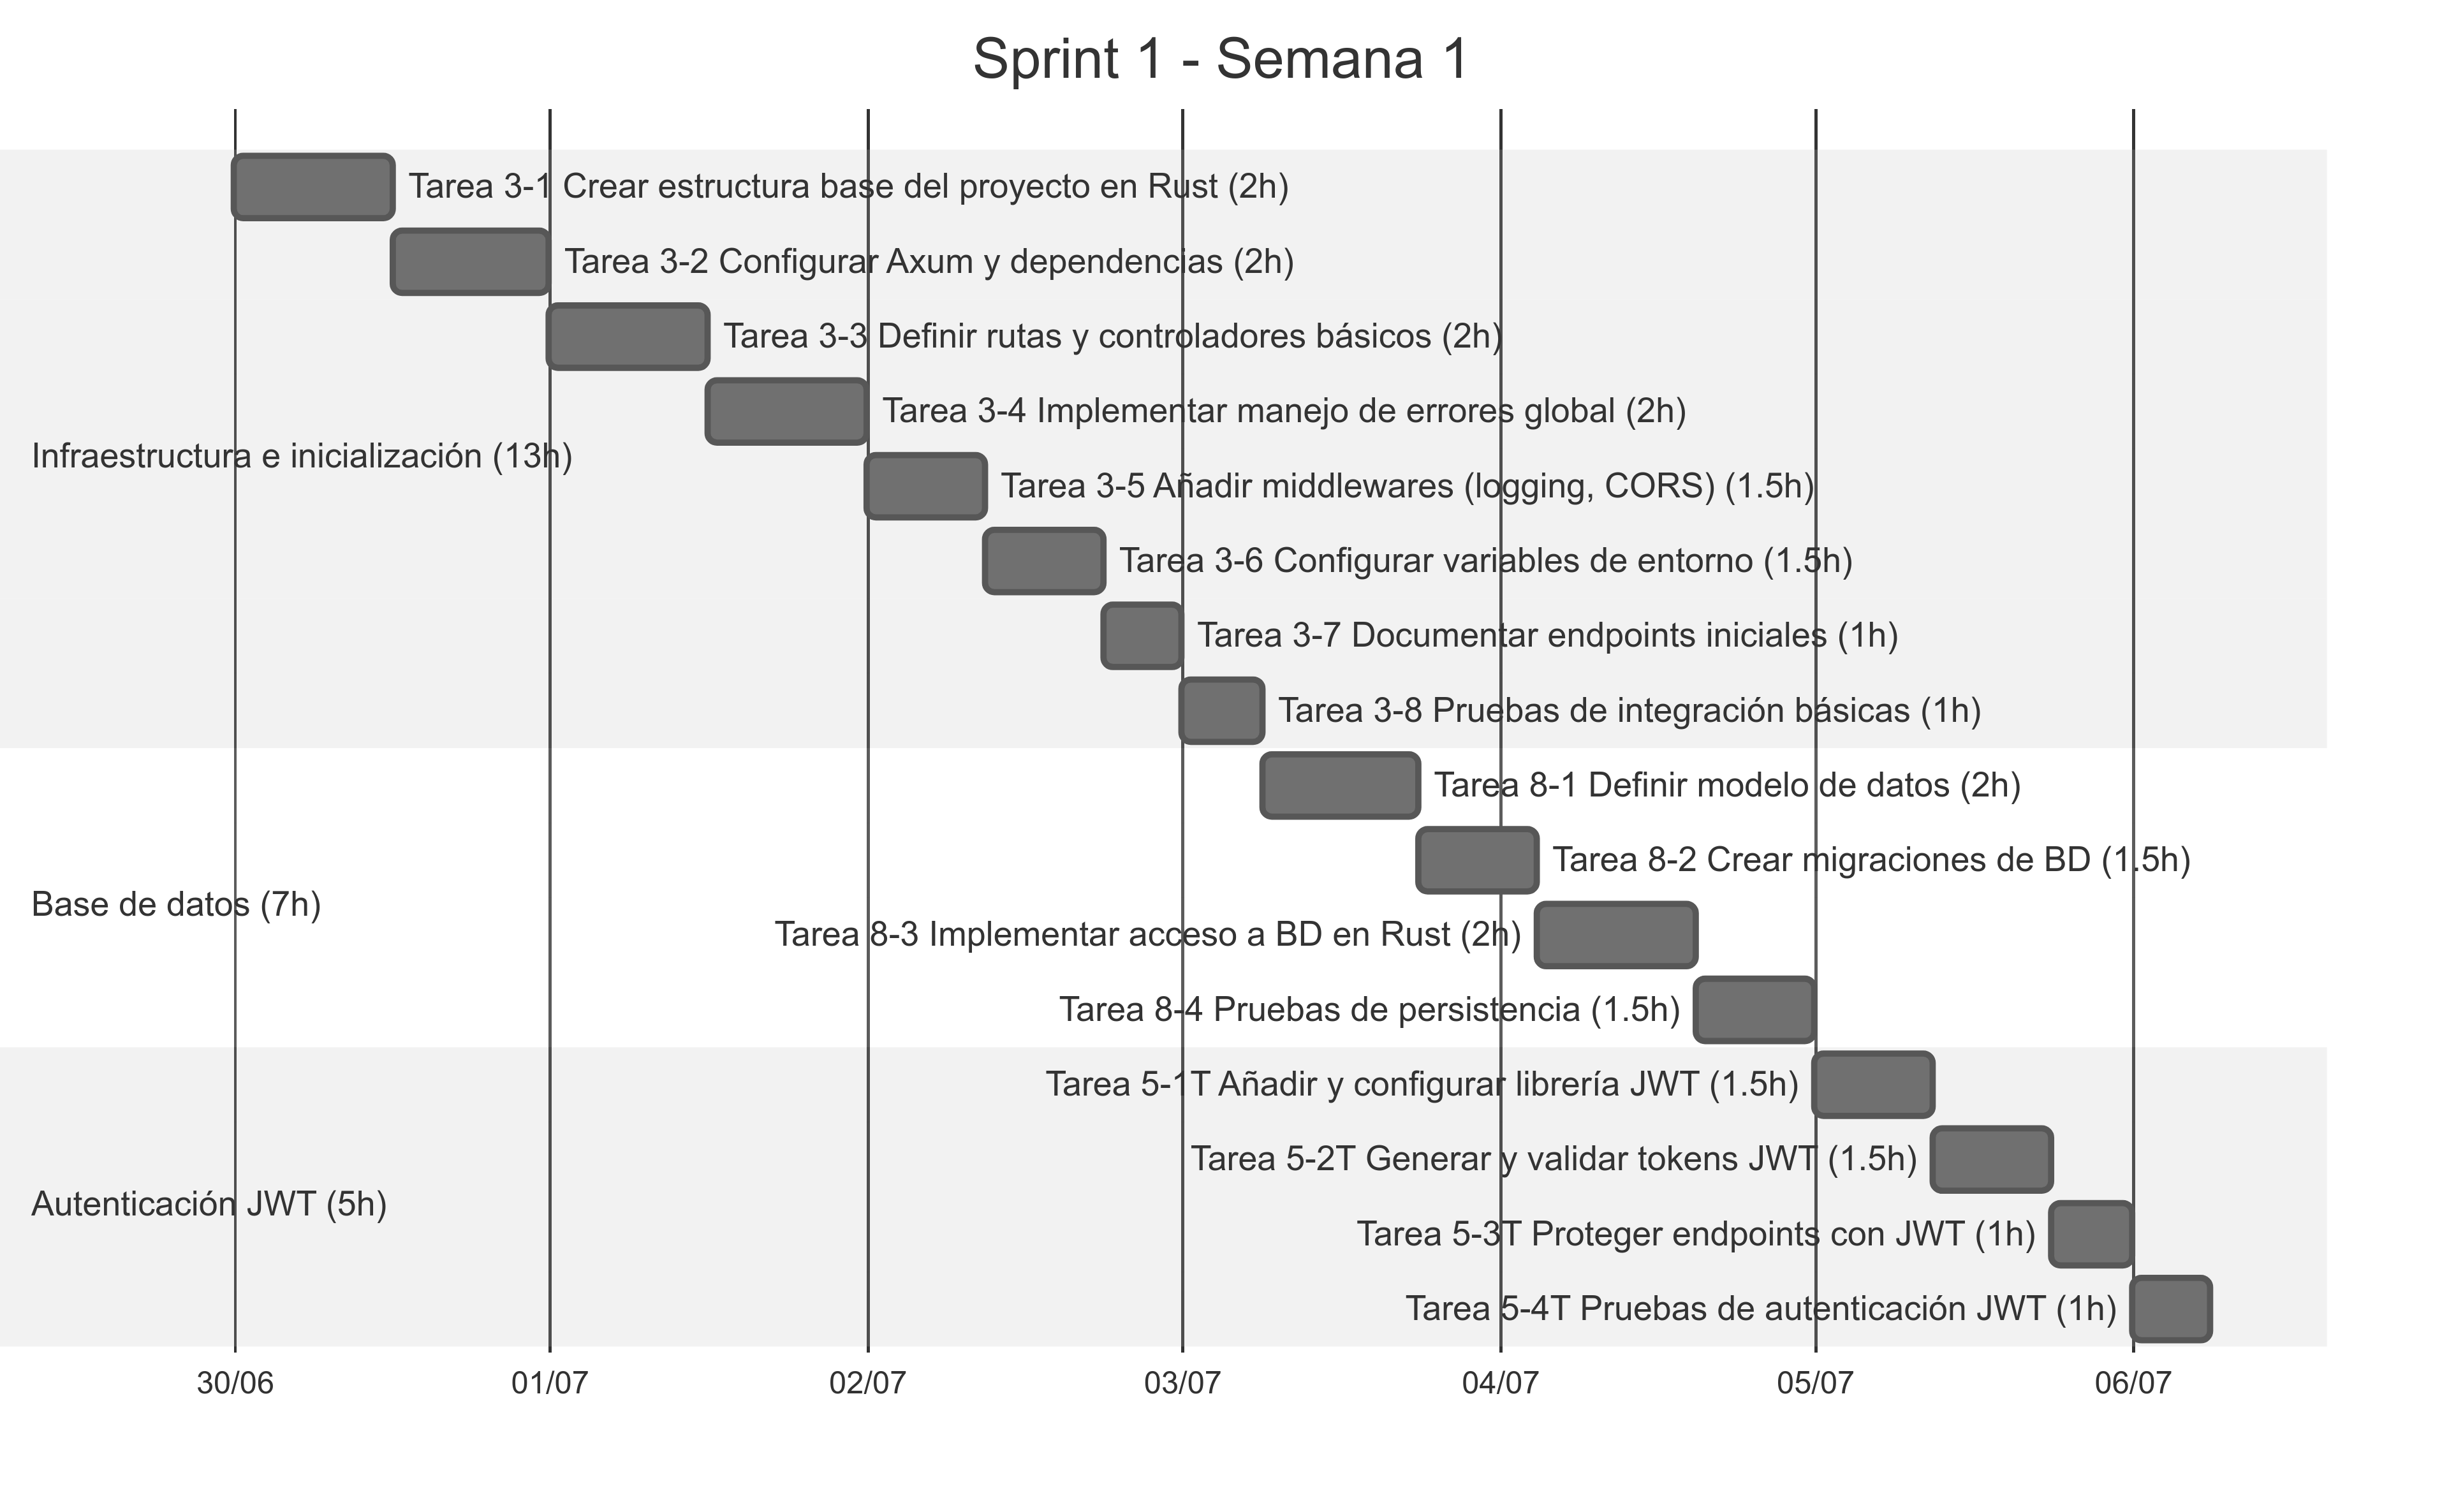
\includegraphics[width=0.8\textwidth]{assets/sprint1/sprint1-week1.png}
    \end{center}
    \caption{Diagrama de Gantt de las tareas de la primera semana del sprint 1}\label{fig:sprint1-week1}
\end{figure}

\begin{figure}[H]
    \begin{center}
        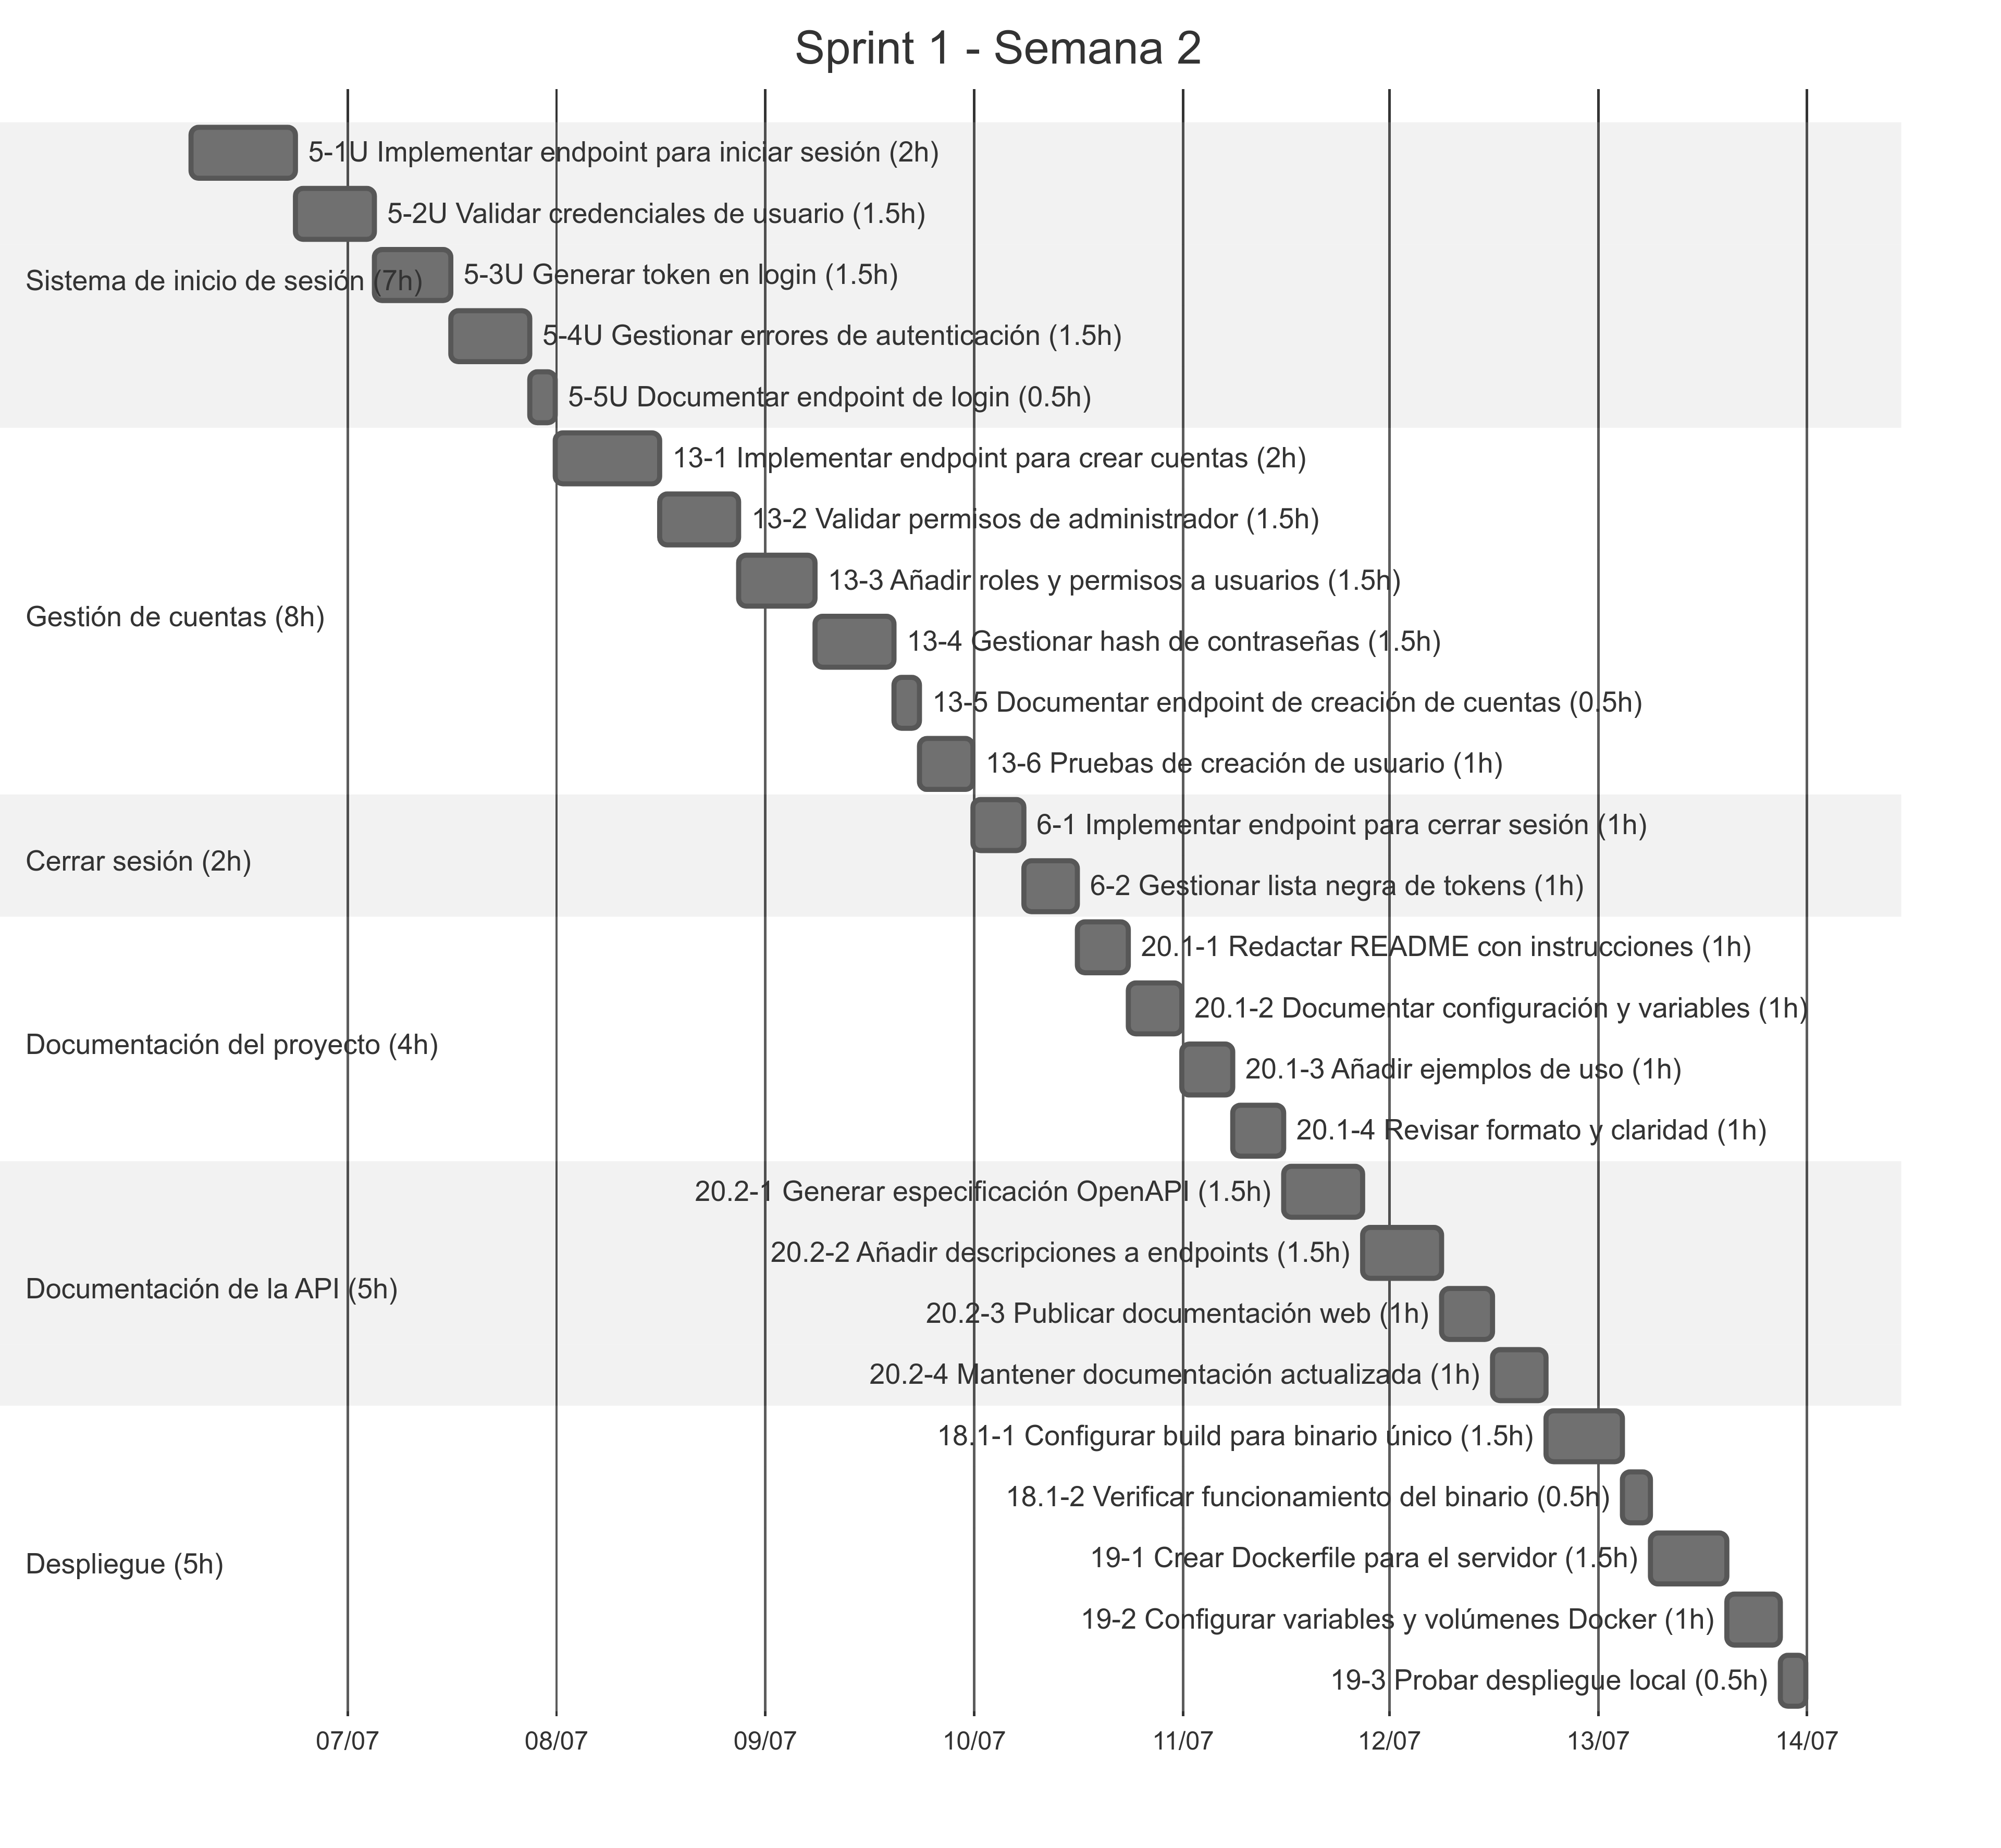
\includegraphics[width=0.8\textwidth]{assets/sprint1/sprint1-week2.png}
    \end{center}
    \caption{Diagrama de Gantt de las tareas de la segunda semana del sprint 1}\label{fig:sprint1-week2}
\end{figure}

Se ha seguido un orden lógico, en el que primero inicializaremos toda la capa de interfaz, en este caso nuestra API, junto con todas las dependencias que nos harán falta a la hora de documentar, errores no genéricos, variables de entorno, pruebas...

Después, se implementará el diseño de la base de datos. Una vez tenemos esta base, se implementarán las primeras funcionalidades, que van a ser la del inicio de sesión seguro, seguido de la gestión de cuentas. Para finalizar el sprint, se documentará todo al completo.

Para finalizar, configuraremos todo lo necesario para poder desplegar el servidor.

\subsection{Diseño detallado e implementación}

\paragraph{Acceso a datos}
\subparagraph{}
Se ha optado por usar el \acrshort{orm} \textbf{Diesel} para el acceso a datos, ya que es uno de los más populares y robustos en el ecosistema de Rust. Diesel proporciona una interfaz segura y eficiente para interactuar con bases de datos SQL, lo que facilita la creación y gestión de esquemas, así como la ejecución de consultas.

Diesel nos proporciona un sistema de migraciones que nos permite versionar y gestionar los cambios en la estructura de la base de datos de manera controlada, generando esquemas que podemos utilizar a la hora de utilizar los métodos que nos proporciona el ORM. De esta manera, tendremos consultas seguras y tipadas.
Esto nos da una especial seguridad a la hora de hacer un desarrollo ágil, ya que podemos iterar rápidamente sobre el modelo de datos y asegurarnos de que los cambios se reflejan correctamente en la base de datos y en nuestro código, ya que hasta que no se solucionen los problemas de compilación provenientes de los cambios en la infraestructura, no se podrá seguir avanzando.

\paragraph{Implementación de Arquitectura Limpia}
\subparagraph{}

Tal y como se ha descrito en apartados anteriores, se ha seguido una arquitectura limpia siguiendo el paradigma de programación \acrshort{cqrs}.

Para ello, se ha aprovechado el sistema de \textit{tipos genéricos} que ofrece Rust.

Los tipos genéricos en Rust permiten escribir código que puede funcionar con múltiples tipos de datos sin necesidad de duplicar el código. Se definen utilizando parámetros de tipo, que son identificadores que se reemplazan por tipos concretos cuando se utiliza el código genérico.

En una arquitectura limpia, los tipos genéricos facilitan la creación de componentes reutilizables e independientes de la implementación concreta. Por ejemplo, se puede definir una interfaz (trait en Rust) para un repositorio de datos y luego implementar diferentes repositorios (e.g., uno para una base de datos y otro para un archivo) que implementen ese trait. Los tipos genéricos permiten que las capas superiores de la aplicación interactúen con el repositorio a través del trait, sin necesidad de conocer la implementación concreta. Esto facilita la inyección de dependencias, donde se puede pasar una implementación concreta del repositorio a la capa superior en tiempo de ejecución.

Los traits en Rust definen un conjunto de métodos que un tipo debe implementar para ser considerado como una instancia de ese trait, se podría considerar que son las ``interfaces'' de Rust. Los traits se pueden usar con tipos genéricos para restringir los tipos que se pueden usar con una función o estructura genérica. Por ejemplo, se puede definir una función genérica que solo funcione con tipos que implementen el trait `Display`.

De esta manera, definimos los traits que nos van a hacer falta en el dominio y cuando queremos usarlo en alguna función, simplemente le pasamos el tipo genérico que está definido en el dominio.
A la hora de inicializar nuestra aplicación es cuando vamos a instanciar los tipos concretos que implementan esos traits que vamos a usar, los cuales se van a inyectar en donde haga falta, por lo general en un estado global de la aplicación, el cual es accesible desde cualquier hilo de ejecución.

Esto se puede ver en el siguiente ejemplo, donde definimos un trait que representa un repositorio de usuarios y luego implementamos el repositorio que accederá a la base de datos mediante el ORM \textbf{Diesel}:

\begin{lstlisting}[language=Rust, caption={Trait de repositorio de usuarios}, label={lst:trait-repository}]
// src/lib/users/domain/user_repository.rs
use std::future::Future;

use crate::users::domain::{user::NewUser, User};

pub trait UserRepository: Clone + Send + Sync + 'static {
    fn get_by_username(
        &self,
        username: String,
    ) -> impl Future<Output = Result<Option<User>, UserRepositoryError>> + Send;
    fn create_user(&self, user: NewUser) -> impl Future<Output = Result<User, UserRepositoryError>> + Send;
}

#[derive(Debug, thiserror::Error)]
pub enum UserRepositoryError {
    #[error("User already exists")]
    UserAlreadyExists,
    #[error("Unexpected error")]
    InternalServerError,
}
\end{lstlisting}
Hemos definido un trait que será usado para acceder de alguna manera que nuestra capa de aplicación no va a saber. Además, se definen errores de dominio, los cuales no tienen nada que ver con cualquier error que pueda ocurrir al acceder a los datos en la base de datos o el sistema que se esté usando.

Además, el trait especifica que su implementación debe también implementar Clone, Send y Sync, asegurando que se pueda utilizar de manera segura entre hilos. Esto es importante para que nuestro repositorio pueda ser usado en un entorno asíncrono y concurrente.

\begin{lstlisting}[language=Rust, caption={Implementación del repositorio de usuarios}, label={lst:impl-repository}]
// src/lib/users/infrastructure/diesel_user_repository.rs
#[derive(Clone)]
pub struct DieselUserRepository {
    pool: Arc<Pool<ConnectionManager<PgConnection>>>,
}

impl DieselUserRepository {
    pub fn new(connection: Arc<Pool<ConnectionManager<PgConnection>>>) -> Self {
        DieselUserRepository { pool: connection }
    }
}

impl UserRepository for DieselUserRepository {
    async fn create_user(&self, new_user: NewUser) -> Result<User, UserRepositoryError> {
        // Implementación de la creación de usuario usando diesel
    }

    async fn get_by_username(
        &self,
        user_username: String,
    ) -> Result<Option<User>, UserRepositoryError> {
        // Implementación de la obtención de usuario por nombre de usuario usando diesel
    }
}
\end{lstlisting}

Aquí podemos ver una implementación del trait que hemos definido anteriormente, en este caso para acceder a una base de datos PostgreSQL mediante el ORM \textbf{Diesel}. Esta implementación es la que se inyectará en el estado global de nuestra aplicación cuando se inicialice.
En este caso, el repositorio implementa Send, Sync y Clone derivándolo de Clone, pues todas sus propiedades las implementan también haciendo que el repositorio lo implemente por ende.

El repositorio usará una pool de conexiones, pues al ser usado por varios hilos, necesitamos que cada hilo tenga su propia conexión a la base de datos para evitar bloqueos y problemas de concurrencia.

Una vez tenemos el trait y su implementación, tan solo nos va a quedar inyectar el repositorio en el estado global y utilizar el estado en nuestra capa de aplicación:
\begin{lstlisting}[language=Rust, caption={Inyección del repositorio en el estado global y uso en el comando para crear un usuario}, label={lst:inject-repository}]
// src/bin/server/main.rs
#[tokio::main]
async fn main() -> anyhow::Result<()> {
    dotenvy::dotenv().ok();


    let connection_pool = Arc::new(establish_connection());

    let user_repository = DieselUserRepository::new(connection_pool);

    let server = HttpServer::new(user_repository).await?;

    server.run().await
}

// src/lib/users/interface/http/routes.rs
pub async fn create_user<UR: UserRepository>(
    State(state): State<AppState<UR>>,
    ValidatedJson(body): ValidatedJson<CreateUserCommand>,
) -> Result<(StatusCode, Json<ApiResponseBody<CreateUserResult>>), ApiError> {
    match create_user_command_handler(body, state.user_repository.as_ref()).await {
        Ok(user) => Ok((
            StatusCode::CREATED,
            ApiResponseBody::new(user).into(),
        )),
        Err(err) => match err {
            UserRepositoryError::UserAlreadyExists => Err(ApiError::ConflictError(err.to_string())),
            UserRepositoryError::InternalServerError => Err(ApiError::InternalServerError(err.to_string())),
        },
    }
}

// src/lib/users/application/commands/create_user.rs
pub async fn create_user_command_handler<UR: UserRepository>(
    mut command: CreateUserCommand,
    user_repository: &UR,
) -> Result<CreateUserResult, UserRepositoryError> {

    if user_repository.get_by_username(command.username.clone()).await?.is_some() {
        return Err(UserRepositoryError::UserAlreadyExists);
    }

    let salt = SaltString::generate(&mut OsRng);

    let argon2 = Argon2::default();

    command.password = argon2
        .hash_password(command.password.as_bytes(), &salt)
        .map_err(|_| UserRepositoryError::InternalServerError)?
        .to_string();

    Ok(user_repository.create_user(command.into()).await?.into())
}
\end{lstlisting}

Cuando definimos el estado global que va a extraer nuestro endpoint mediante el extractor que nos proporciona Axum, lo definimos con un tipo genérico \textit{UR}, el cual especificamos que va a implementar el trait \textit{UserRepository}. Es decir, sabemos los métodos que nos ofrece y las propiedades que tiene que tener, pero en la capa de aplicación no tenemos que conocer cómo se está implementando, solamente cómo se usa.

Otra buena práctica que podemos observar en el código es utilizar errores de dominio. De esta manera, abstraemos la capa de aplicación de cualquier tipo de error que pueda ocurrir en la capa de infraestructura y solamente en la capa de interfaz, que es la que presenta los datos al usuario, asociamos cada error de dominio al error correspondiente de interfaz.

Así, si quisiéramos cambiar cómo accedemos a los datos, tan solo tendríamos que crear o modificar la implementación que realizamos en la capa de infraestructura.

El siguiente diagrama muestra cómo se relacionan las diferentes capas de la arquitectura limpia que hemos implementado:
\begin{figure}[H]
    \begin{center}
        \includegraphics[width=0.95\textwidth]{assets/sprint1/diagrama-arquitectura-limpia.png}
    \end{center}
    \caption{Diagrama del diseño arquitectónico detallado de nuestra implementación.}\label{fig:diagrama-arquitectura-limpia-sprint1}
\end{figure}

Tal como se ha definido en la arquitectura software, la capa de interfaz accede a la capa de aplicación pero no viceversa. Para hacer uso de la capa de infraestructura, la capa de aplicación utiliza una abstracción de dominio que utiliza siempre objetos de dominio, la cual después la infraestructura implementa y se inicializa en el estado global de la aplicación.

\paragraph{Documentación de la API REST}
\subparagraph{}

Para documentar todos los endpoints de la API REST, se ha utilizado la especificación OpenAPI. Esta especificación permite describir de manera estructurada los endpoints, parámetros, tipos de datos y respuestas de la API.

Esta documentación se genera automáticamente mediante la librería \textbf{utoipa}, que se integra con Axum para generar la documentación a partir de los atributos y tipos definidos en el código. 
Esto asegura que la documentación esté siempre actualizada y refleje fielmente el estado actual de la API, por lo que cada vez que definamos un nuevo endpoint o modifiquemos uno existente, la documentación se actualizará automáticamente.

Además, se ha configurado otra librería compatible con utoipa \textbf{utoipa-swagger-ui}, que permite servir la documentación generada como una página web interactiva, lo que facilita a los desarrolladores y usuarios explorar y probar los endpoints de la API, mostrando ejemplos de peticiones, respuestas, errores y los esquemas usados en las peticiones y respuestas.
Además, nos permite probar los endpoints directamente desde la interfaz.

\paragraph{Pruebas unitarias y de integración}
\subparagraph{}

Para garantizar la calidad del código y el correcto funcionamiento de la aplicación, se han implementado pruebas unitarias y de integración utilizando la librería \textbf{tokio} para pruebas asíncronas y un \textbf{servicio oneshot} para simular el servidor HTTP.
El servicio oneshot no es más que un servidor HTTP con unas rutas definidas al igual que nuestra API, solo que es de un solo uso para realizar pruebas, ya que solamente deja simular una sola petición y respuesta, lo que es suficiente para nuestras pruebas unitarias.

En este punto es donde entra en juego una de las ventajas de utilizar una arquitectura limpia y CQRS.
Al separar la lógica de negocio de la infraestructura, podemos probar los comandos y consultas de manera aislada, sin necesidad de depender de la implementación concreta del repositorio o de la base de datos. Esto nos permite escribir pruebas más rápidas y enfocadas en la lógica de negocio.

Además, nos da la ventaja de poder \gls{mockear} los repositorios y otros componentes de infraestructura, lo que facilita la simulación de diferentes escenarios y errores en las pruebas.

Así, tendríamos la siguiente estructura en la carpeta de tests:

\dirtree{%
.1 tests.
.2 tests.rs.
.2 users.
.3 application.
.4 commands.
.5 test\_create\_user.rs.
.5 test\_login.rs.
.4 queries.
.5 test\_get\_all\_users.rs.
.5 test\_get\_user.rs.
.3 domain.
.4 auth.rs.
.4 roles.rs.
.4 user\_repository.rs.
.4 user.rs.
.3 infrastructure.
.4 test\_jwt\_token\_service.rs.
.4 test\_mappers.rs.
.4 test\_models.rs.
.4 test\_repository.rs.
.3 integration.
.4 test\_user\_endpoints.rs.
.3 mocks.rs.
.2 utils.
.3 functions.rs.
}

Como se puede ver, hemos separado las pruebas en diferentes carpetas según su tipo: pruebas de dominio, de infraestructura, de aplicación y de integración.
Se han abarcado todos los casos de uso definidos en las historias de usuario, asegurando que cada funcionalidad se prueba de manera aislada y también en conjunto con el resto del sistema.

Para ejecutar todos los tests, es tan sencillo como ejecutar el comando $cargo\ test$ en la raíz del proyecto, lo que ejecutará todas las pruebas definidas en la carpeta \texttt{tests} y mostrará los resultados en la consola.

\paragraph{Despliegue}
\subparagraph{}

Todos los pasos necesarios para el despliegue se han definido en el README del proyecto, donde se explica cómo construir el binario, cómo crear la imagen Docker y cómo ejecutar el servidor en un contenedor Docker, o directamente del binario compilado.

Nuestra aplicación depende de una base de datos PostgreSQL (de momento) y se ha generado un archivo docker compose para facilitar el despliegue de la aplicación junto con la base de datos. Este archivo define los servicios necesarios, incluyendo el servidor y la base de datos, y permite iniciar todo el entorno con un solo comando.

Si bien se puede utilizar docker compose para levantar el entorno de desarrollo, también se puede ejecutar el servidor directamente desde el binario generado, definiendo en las variables de entorno los parámetros necesarios para la base de datos, sin necesidad de usar Docker.

\newpage
\section{Sprint 2}
\label{sec:sprint2}

Siguiendo la planificación inicial detallada en la sección \ref{sec:planificacion-inicial}, el segundo sprint se enfoca exclusivamente en el desarrollo de la \textbf{aplicación móvil}. El objetivo principal es sentar las bases de la aplicación cliente, creando una estructura de proyecto robusta, implementando los módulos nativos necesarios para funcionalidades clave y desarrollando una primera versión de la interfaz de usuario.

El entregable al final de este sprint será una aplicación de galería básica que pueda solicitar los permisos necesarios, acceder a las fotos y vídeos del dispositivo y mostrarlos en una interfaz de usuario funcional. Aún no se implementarán las funcionalidades de sincronización con el servidor, ya que el foco está en la arquitectura del cliente y su interacción con el sistema operativo móvil.

La velocidad del equipo del sprint anterior se utilizará como referencia, pero al cambiar completamente el contexto de desarrollo (de backend a móvil), se asume una incertidumbre similar a la del primer sprint. La selección de historias se ha realizado buscando un equilibrio entre la creación de la estructura fundamental y la implementación de una primera funcionalidad visible.

\subsection{Historias de usuario}
A continuación, se presentan las historias de usuario y técnicas seleccionadas para este sprint, priorizando la creación del esqueleto de la aplicación móvil y la interacción con el sistema nativo.

Las historias seleccionadas son las siguientes:
\begin{itemize}
    \item HU20: Ver archivos subidos (adaptada a "Ver archivos locales") - 5 PH
    \item HU24: Inicio y cierre de sesión - 5 PH
    \item HU25: Gestión de permisos - 3 PH
    \item HT23: Acceso a la galería - 5 PH
    \item HT24: Comunicación con API - 5 PH
    \item HT29: Pruebas unitarias - 5 PH (parcial)
    \item HT31: Gestión de tokens - 3 PH
    \item HT36: UI responsive - 3 PH
\end{itemize}

La suma total de las historias seleccionadas es de \textbf{34 puntos de historia (PH)}. Aunque el número de puntos es menor que en el sprint anterior, la complejidad de configurar un nuevo entorno de desarrollo móvil y la implementación de módulos nativos justifica una carga de trabajo similar.

Además, se estima una carga extra a la hora de implementar los módulos nativos y la integración con Lynx.js, lo que puede hacer que el esfuerzo real sea comparable al del primer sprint.

\subsection{Descomposición en tareas de desarrollo}

% HU20: Ver archivos subidos (adaptada)
\begin{table}[H]
    \begin{center}
        \begin{tabularx}{\textwidth}{|l|X|l|}
            \hline
            \textbf{Identificador HU20} &
            \textbf{Como usuario, quiero ver una lista o galería de los archivos que ya están en mi dispositivo} &
            \textbf{Estimación: 5 PH}\\
            \hline
            \multicolumn{3}{|p{\textwidth}|}{
                \begin{minipage}{\textwidth}
                    \centering
                    \vspace{0.5em}
                    \begin{tabular}{|l|p{8cm}|r|}
                        \hline
                        \textbf{Identificador} & \textbf{Título de la tarea de desarrollo} & \makecell{\textbf{Estimación}\\\textbf{(h)}} \\
                        \hline
                        Tarea 20-1 & Crear el componente de la pantalla principal (galería) & 4.5 \\
                        \hline
                        Tarea 20-2 & Implementar un componente para previsualizar cada imagen (thumbnail) & 4 \\
                        \hline
                        Tarea 20-3 & Diseñar y maquetar una cuadrícula (grid) para mostrar las imágenes & 2 \\
                        \hline
                        Tarea 20-4 & Integrar la lógica para obtener las imágenes del dispositivo (depende de HT23) & 3 \\
                        \hline
                    \end{tabular}
                    \vspace{0.5em}
                \end{minipage}
            } \\
            \hline
            \multicolumn{3}{|p{\textwidth}|}{
                \textbf{Pruebas de aceptación:}
                \begin{itemize}
                    \item Al abrir la app (tras iniciar sesión), se muestra una galería con las imágenes del móvil.
                    \item Las imágenes se muestran en una cuadrícula ordenada.
                    \item La interfaz es fluida al desplazarse por la galería.
                \end{itemize}
            }\\
            \hline
            \multicolumn{3}{|p{\textwidth}|}{
                \textbf{Observaciones:}
                \begin{itemize}
                    \item La historia original era ``ver archivos subidos'', pero se adapta para este sprint a ``ver archivos locales'' como primer paso.
                    \item Inicialmente no se incluirá la carga de vídeos, solo imágenes.
                \end{itemize}
            }\\
            \hline
        \end{tabularx}
    \end{center}
\end{table}

% HU24: Inicio y cierre de sesión
\begin{table}[H]
    \begin{center}
        \begin{tabularx}{\textwidth}{|l|X|l|}
            \hline
            \textbf{Identificador HU24} &
            \textbf{Como usuario, quiero iniciar y cerrar sesión para proteger mis datos} &
            \textbf{Estimación: 5 PH}\\
            \hline
            \multicolumn{3}{|p{\textwidth}|}{
                \begin{minipage}{\textwidth}
                    \centering
                    \vspace{0.5em}
                    \begin{tabular}{|l|p{8cm}|r|}
                        \hline
                        \textbf{Identificador} & \textbf{Título de la tarea de desarrollo} & \makecell{\textbf{Estimación}\\\textbf{(h)}} \\
                        \hline
                        Tarea 24-1U & Diseñar y maquetar la pantalla de inicio de sesión & 2 \\
                        \hline
                        Tarea 24-2U & Implementar la lógica del formulario (usuario, contraseña) & 1.5 \\
                        \hline
                        Tarea 24-3U & Integrar la llamada al endpoint de login del servidor (depende de HT24) & 2 \\
                        \hline
                        Tarea 24-4U & Implementar la navegación: si el login es exitoso, ir a la galería & 1 \\
                        \hline
                        Tarea 24-5U & Añadir un botón para cerrar sesión que borre el token (depende de HT31) & 1 \\
                        \hline
                    \end{tabular}
                    \vspace{0.5em}
                \end{minipage}
            } \\
            \hline
            \multicolumn{3}{|p{\textwidth}|}{
                \textbf{Pruebas de aceptación:}
                \begin{itemize}
                    \item El usuario puede introducir sus credenciales y pulsar un botón para iniciar sesión.
                    \item Si las credenciales son válidas, se le redirige a la pantalla de la galería.
                    \item Si son inválidas, se muestra un mensaje de error.
                    \item Existe una opción para cerrar la sesión actual.
                \end{itemize}
            }\\
            \hline
            \multicolumn{3}{|p{\textwidth}|}{
                \textbf{Observaciones:}
                \begin{itemize}
                    \item Esta HU conecta el cliente con el backend desarrollado en el Sprint 1.
                \end{itemize}
            }\\
            \hline
        \end{tabularx}
    \end{center}
\end{table}

% HU25: Gestión de permisos
\begin{table}[H]
    \begin{center}
        \begin{tabularx}{\textwidth}{|l|X|l|}
            \hline
            \textbf{Identificador HU25} &
            \textbf{Como usuario, quiero que la app me pida permisos de acceso solo cuando sea necesario} &
            \textbf{Estimación: 3 PH}\\
            \hline
            \multicolumn{3}{|p{\textwidth}|}{
                \begin{minipage}{\textwidth}
                    \centering
                    \vspace{0.5em}
                    \begin{tabular}{|l|p{8cm}|r|}
                        \hline
                        \textbf{Identificador} & \textbf{Título de la tarea de desarrollo} & \makecell{\textbf{Estimación}\\\textbf{(h)}} \\
                        \hline
                        Tarea 25-1 & Implementar la lógica para verificar si los permisos ya han sido concedidos & 1 \\
                        \hline
                        Tarea 25-2 & Invocar el diálogo nativo de solicitud de permisos de lectura de almacenamiento & 1.5 \\
                        \hline
                        Tarea 25-3 & Gestionar la respuesta del usuario (permiso concedido o denegado) & 1.5 \\
                        \hline
                    \end{tabular}
                    \vspace{0.5em}
                \end{minipage}
            } \\
            \hline
            \multicolumn{3}{|p{\textwidth}|}{
                \textbf{Pruebas de aceptación:}
                \begin{itemize}
                    \item Al intentar acceder a la galería por primera vez, la app solicita permiso para leer el almacenamiento.
                    \item Si el usuario concede el permiso, la app muestra las imágenes.
                    \item Si el usuario deniega el permiso, la app muestra un mensaje informativo.
                \end{itemize}
            }\\
            \hline
            \multicolumn{3}{|p{\textwidth}|}{
                \textbf{Observaciones:}
                \begin{itemize}
                    \item Esta historia está ligada a la implementación del módulo nativo (HT23).
                \end{itemize}
            }\\
            \hline
        \end{tabularx}
    \end{center}
\end{table}

% HT23: Acceso a la galería
\begin{table}[H]
    \begin{center}
        \begin{tabularx}{\textwidth}{|l|X|l|}
            \hline
            \textbf{Identificador HT23} &
            \textbf{Implementar acceso seguro a la galería de fotos y vídeos} &
            \textbf{Estimación: 5 PH}\\
            \hline
            \multicolumn{3}{|p{\textwidth}|}{
                \begin{minipage}{\textwidth}
                    \centering
                    \vspace{0.5em}
                    \begin{tabular}{|l|p{8cm}|r|}
                        \hline
                        \textbf{Identificador} & \textbf{Título de la tarea de desarrollo} & \makecell{\textbf{Estimación}\\\textbf{(h)}} \\
                        \hline
                        Tarea 23-1 & Configurar el proyecto `Lynx Explorer' para añadir un módulo nativo en Android & 3 \\
                        \hline
                        Tarea 23-2 & Escribir el código nativo (Java/Kotlin) para consultar el `MediaStore' de Android & 3 \\
                        \hline
                        Tarea 23-3 & Crear el ``puente'' (bridge) para exponer la funcionalidad nativa a JavaScript & 2.5 \\
                        \hline
                        Tarea 23-4 & Implementar el método en JS que llama al módulo nativo para obtener las URIs de las imágenes & 2 \\
                        \hline
                    \end{tabular}
                    \vspace{0.5em}
                \end{minipage}
            } \\
            \hline
            \multicolumn{3}{|p{\textwidth}|}{
                \textbf{Pruebas de aceptación:}
                \begin{itemize}
                    \item El código JavaScript puede invocar una función que devuelve una lista de imágenes del dispositivo.
                    \item El módulo nativo gestiona correctamente los permisos y errores de acceso.
                    \item La app puede compilarse con el nuevo módulo nativo incluido.
                \end{itemize}
            }\\
            \hline
            \multicolumn{3}{|p{\textwidth}|}{
                \textbf{Observaciones:}
                \begin{itemize}
                    \item Esta es una de las tareas más complejas y críticas del sprint, ya que valida el uso de una de las características clave de Lynx.js.
                \end{itemize}
            }\\
            \hline
        \end{tabularx}
    \end{center}
\end{table}


% HT24: Comunicación con API
\begin{table}[H]
    \begin{center}
        \begin{tabularx}{\textwidth}{|l|X|l|}
            \hline
            \textbf{Identificador HT24} &
            \textbf{Integrar cliente HTTP que se comunique con el servidor} &
            \textbf{Estimación: 5 PH}\\
            \hline
            \multicolumn{3}{|p{\textwidth}|}{
                \begin{minipage}{\textwidth}
                    \centering
                    \vspace{0.5em}
                    \begin{tabular}{|l|p{8cm}|r|}
                        \hline
                        \textbf{Identificador} & \textbf{Título de la tarea de desarrollo} & \makecell{\textbf{Estimación}\\\textbf{(h)}} \\
                        \hline
                        Tarea 24-1 & Seleccionar e instalar una librería de cliente HTTP (ej. axios) & 0.5 \\
                        \hline
                        Tarea 24-2 & Crear una capa de servicio (service layer) para encapsular las llamadas a la API & 2 \\
                        \hline
                        Tarea 24-3 & Definir los \glspl{dto} para las peticiones y respuestas & 1.5 \\
                        \hline
                        Tarea 24-4 & Implementar la lógica para añadir el token JWT a las cabeceras de las peticiones & 1.5 \\
                        \hline
                    \end{tabular}
                    \vspace{0.5em}
                \end{minipage}
            } \\
            \hline
            \multicolumn{3}{|p{\textwidth}|}{
                \textbf{Pruebas de aceptación:}
                \begin{itemize}
                    \item La aplicación puede realizar una petición POST al endpoint de login.
                    \item Se puede configurar la URL base del servidor mediante variables de entorno (en sprints posteriores, esta url se descubrirá automáticamente en la red).
                    \item La capa de servicio maneja correctamente las respuestas exitosas y de error.
                \end{itemize}
            }\\
            \hline
            \multicolumn{3}{|p{\textwidth}|}{
                \textbf{Observaciones:}
                \begin{itemize}
                    \item La implementación seguirá los principios de la arquitectura limpia, aislando la infraestructura de red.
                \end{itemize}
            }\\
            \hline
        \end{tabularx}
    \end{center}
\end{table}

% HT29: Pruebas unitarias
\begin{table}[H]
    \begin{center}
        \begin{tabularx}{\textwidth}{|l|X|l|}
            \hline
            \textbf{Identificador HT29} &
            \textbf{Añadir pruebas unitarias y de integración a la lógica común en React / Lynx.js} &
            \textbf{Estimación: 5 PH (Parcial)}\\
            \hline
            \multicolumn{3}{|p{\textwidth}|}{
                \begin{minipage}{\textwidth}
                    \centering
                    \vspace{0.5em}
                    \begin{tabular}{|l|p{8cm}|r|}
                        \hline
                        \textbf{Identificador} & \textbf{Título de la tarea de desarrollo} & \makecell{\textbf{Estimación}\\\textbf{(h)}} \\
                        \hline
                        Tarea 29-1 & Configurar el entorno de pruebas (Jest) & 2 \\
                        \hline
                        Tarea 29-2 & Escribir pruebas para los servicios de la capa de aplicación (ej. servicio de autenticación) & 2.5 \\
                        \hline
                    \end{tabular}
                    \vspace{0.5em}
                \end{minipage}
            } \\
            \hline
            \multicolumn{3}{|p{\textwidth}|}{
                \textbf{Pruebas de aceptación:}
                \begin{itemize}
                    \item Se pueden ejecutar las pruebas desde la línea de comandos.
                    \item Los componentes visuales tienen pruebas que verifican su renderizado y comportamiento.
                    \item La lógica de negocio está cubierta por pruebas unitarias.
                    \item Las dependencias externas (API, módulos nativos) están mockeadas en las pruebas.
                \end{itemize}
            }\\
            \hline
            \multicolumn{3}{|p{\textwidth}|}{
                \textbf{Observaciones:}
                \begin{itemize}
                    \item Es una historia técnica de alta estimación porque establecer una buena base de pruebas desde el principio es fundamental para la mantenibilidad del proyecto.
                \end{itemize}
            }\\
            \hline
        \end{tabularx}
    \end{center}
\end{table}

% HT31: Gestión de tokens
\begin{table}[H]
    \begin{center}
        \begin{tabularx}{\textwidth}{|l|X|l|}
            \hline
            \textbf{Identificador HT31} &
            \textbf{Almacenar y renovar tokens de autenticación de forma segura} &
            \textbf{Estimación: 3 PH}\\
            \hline
            \multicolumn{3}{|p{\textwidth}|}{
                \begin{minipage}{\textwidth}
                    \centering
                    \vspace{0.5em}
                    \begin{tabular}{|l|p{8cm}|r|}
                        \hline
                        \textbf{Identificador} & \textbf{Título de la tarea de desarrollo} & \makecell{\textbf{Estimación}\\\textbf{(h)}} \\
                        \hline
                        Tarea 31-1 & Investigar y elegir una solución de almacenamiento seguro local (ej. AsyncStorage) & 1 \\
                        \hline
                        Tarea 31-2 & Crear un servicio para guardar, leer y eliminar el token JWT del almacenamiento & 2 \\
                        \hline
                        Tarea 31-3 & Integrar este servicio en el flujo de inicio y cierre de sesión & 1 \\
                        \hline
                    \end{tabular}
                    \vspace{0.5em}
                \end{minipage}
            } \\
            \hline
            \multicolumn{3}{|p{\textwidth}|}{
                \textbf{Pruebas de aceptación:}
                \begin{itemize}
                    \item Tras un inicio de sesión exitoso, el token JWT se guarda en el dispositivo.
                    \item Al cerrar la aplicación y volver a abrirla, el usuario sigue autenticado (se recupera el token).
                    \item Al cerrar sesión, el token se elimina del almacenamiento.
                \end{itemize}
            }\\
            \hline
        \end{tabularx}
    \end{center}
\end{table}

% HT36: UI responsive
\begin{table}[H]
    \begin{center}
        \begin{tabularx}{\textwidth}{|l|X|l|}
            \hline
            \textbf{Identificador HT36} &
            \textbf{Adaptar UI para distintos tamaños de pantalla (tablet, móvil)} &
            \textbf{Estimación: 3 PH}\\
            \hline
            \multicolumn{3}{|p{\textwidth}|}{
                \begin{minipage}{\textwidth}
                    \centering
                    \vspace{0.5em}
                    \begin{tabular}{|l|p{8cm}|r|}
                        \hline
                        \textbf{Identificador} & \textbf{Título de la tarea de desarrollo} & \makecell{\textbf{Estimación}\\\textbf{(h)}} \\
                        \hline
                        Tarea 36-1 & Implementar una estrategia de diseño adaptable & 2 \\
                        \hline
                        Tarea 36-2 & Probar y ajustar la UI de la galería y el login en emuladores de tablet y móvil & 2 \\
                        \hline
                    \end{tabular}
                    \vspace{0.5em}
                \end{minipage}
            } \\
            \hline
            \multicolumn{3}{|p{\textwidth}|}{
                \textbf{Pruebas de aceptación:}
                \begin{itemize}
                    \item La pantalla de login se ve correctamente tanto en un móvil de tamaño estándar como en una tablet.
                    \item La cuadrícula de la galería adapta el número de columnas según el ancho de la pantalla.
                \end{itemize}
            }\\
            \hline
        \end{tabularx}
    \end{center}
\end{table}

\paragraph{Resumen de estimación de tareas}

El total de horas estimadas para las tareas de desarrollo del Sprint 2 es de \textbf{53.5 horas}, cifra que se acerca a la capacidad teórica del sprint (56 horas). La distribución es la siguiente:

\begin{itemize}
    \item HU20 (Ver archivos locales): 13.5 horas
    \item HU24 (Inicio y cierre de sesión): 7.5 horas
    \item HU25 (Gestión de permisos): 4 horas
    \item HT23 (Acceso a la galería): 10.5 horas
    \item HT24 (Comunicación con API): 5.5 horas
    \item HT29 (Pruebas unitarias): 4.5 horas
    \item HT31 (Gestión de tokens): 4 horas
    \item HT36 (UI responsive): 4 horas
\end{itemize}

Se observa que historias técnicas como HT23 (módulo nativo) y HU20 (archivos locales) consumen una parte significativa del tiempo. Esto se debe a la complejidad de implementar módulos nativos y establecer una base sólida para la aplicación móvil. El desarrollo de los módulos nativos se realiza en Kotlin/Java, entorno en el que el equipo no tiene ninguna experiencia previa.

\subsection{Diagrama de Gantt}
A la hora de realizar las tareas se ha priorizado la visualización de una galería funcional en la aplicación. Una vez que se tenga una galería funcional, se implementarán las funcionalidades que tienen que ver con la comunicación con la API. El acceso a la galería (HT23) es una tarea crítica que debe completarse antes de poder implementar la visualización de archivos locales (HU20), es por ello que las tareas relacionadas con la historia técnica van antes que las de la historia de usuario.

\begin{figure}[H]
    \begin{center}
        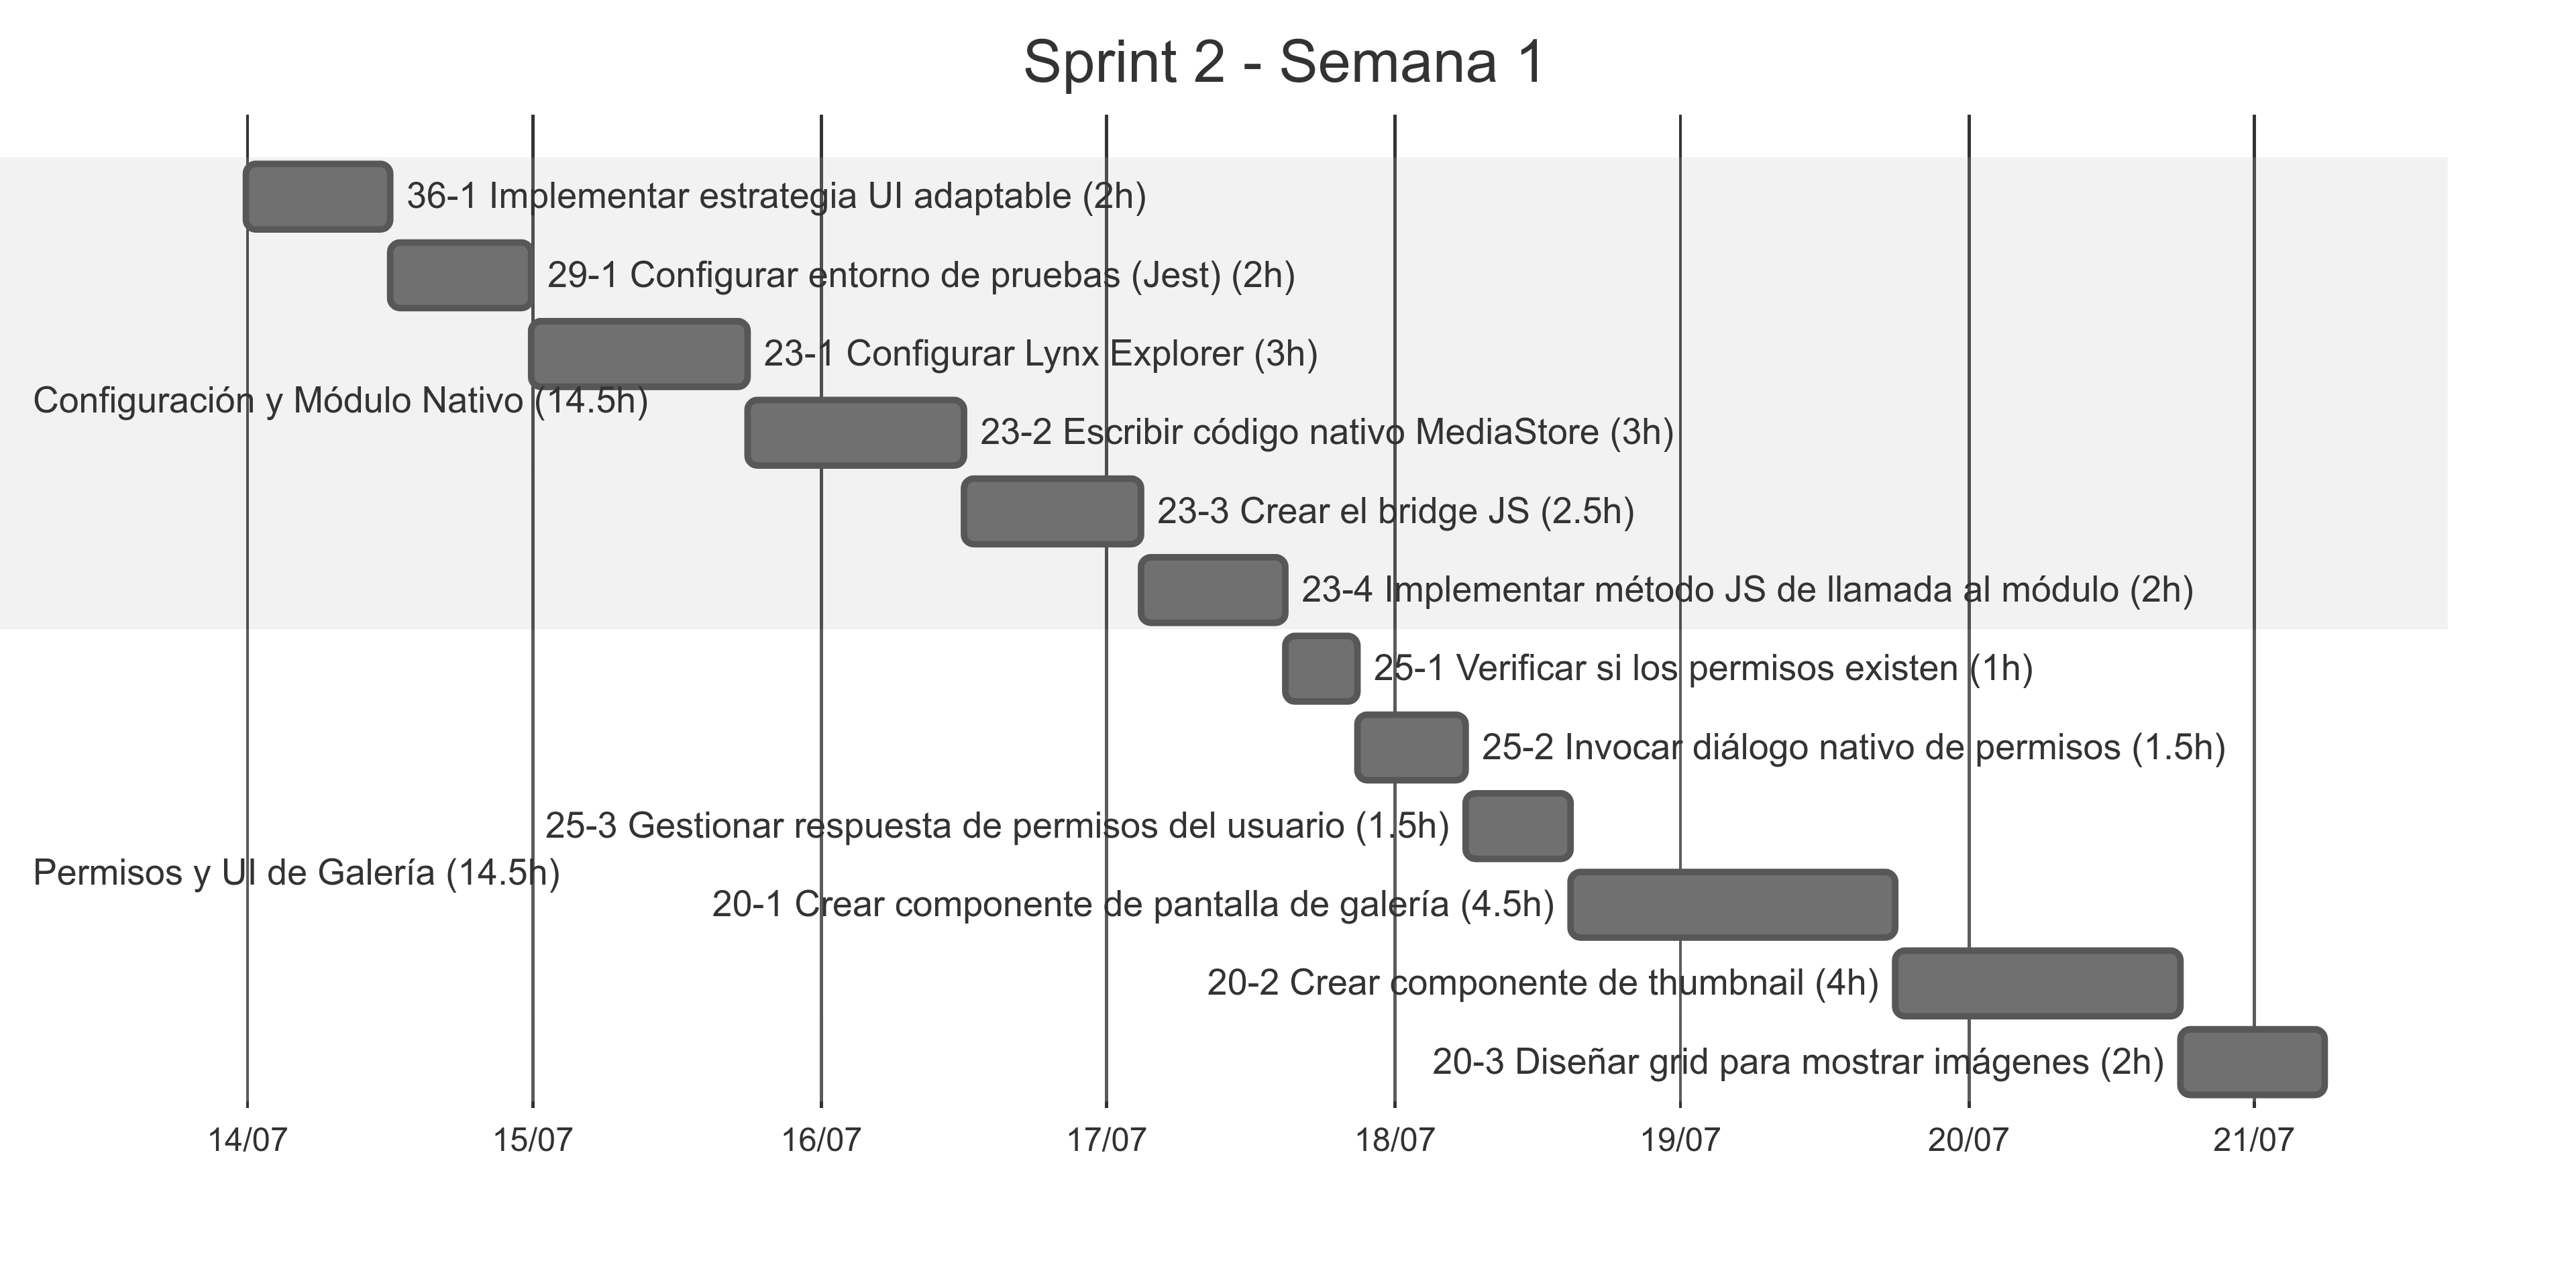
\includegraphics[width=0.8\textwidth]{assets/sprint2/week1-gantt.png}
    \end{center}
    \caption{Diagrama de Gantt de las tareas de la primera semana del sprint 2}\label{fig:gantt-sprint2-week1}
\end{figure}

\begin{figure}[H]
    \begin{center}
        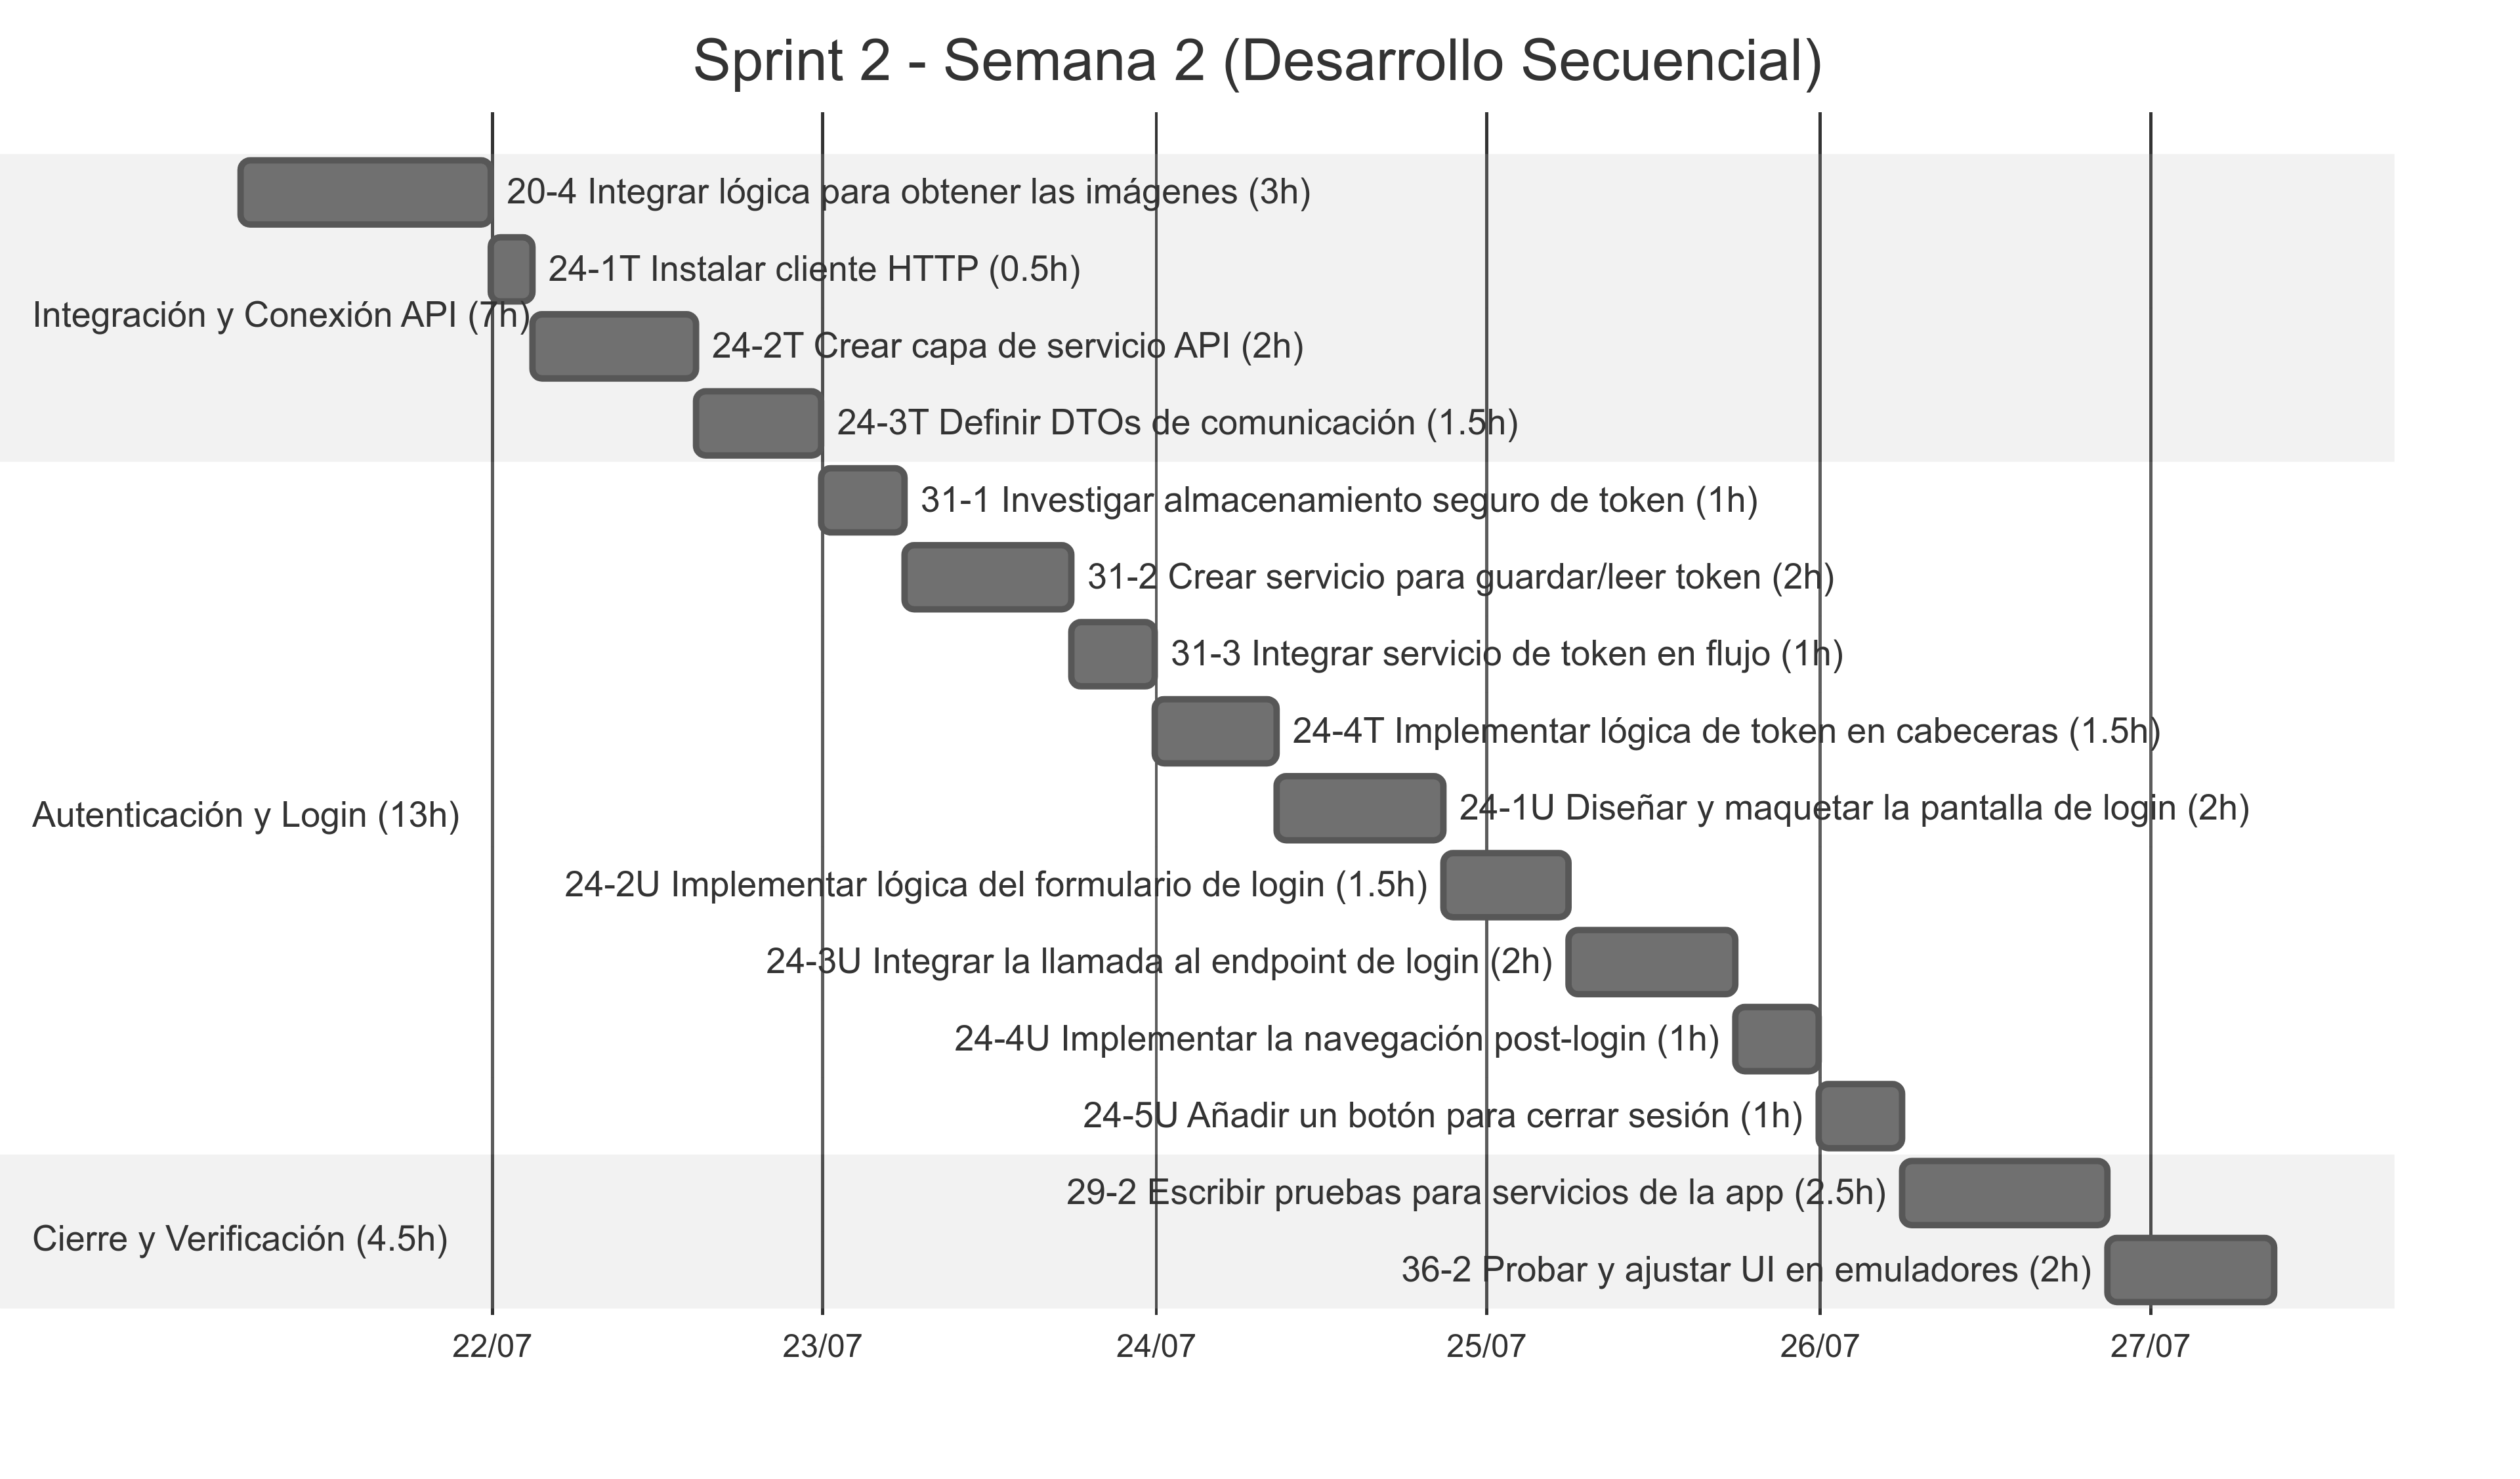
\includegraphics[width=0.8\textwidth]{assets/sprint2/week2-gantt.png}
    \end{center}
    \caption{Diagrama de Gantt de las tareas de la segunda semana del sprint 2}\label{fig:gantt-sprint2-week2}
\end{figure}


\subsection{Diseño detallado e implementación}

\paragraph{Arquitectura del Cliente Móvil}
\subparagraph{}
Como se definió en la propuesta, la aplicación móvil seguirá los principios de la \textbf{Arquitectura Limpia}. Durante este sprint se materializará esta estructura creando los siguientes directorios y capas lógicas:
\begin{itemize}
    \item \textbf{Presentation}: Contendrá todos los componentes de React (Lynx.js), las pantallas (Login, Galería), y los hooks visuales. Es la capa más externa.
    \item \textbf{Domain}: Albergará las entidades de negocio (ej. `User', `MediaFile') y las definiciones de las interfaces de los repositorios (ej. `AuthRepository', `MediaRepository'). Esta capa no tendrá dependencias externas.
    \item \textbf{Application}: Contendrá los casos de uso (ej. `loginUser', `getLocalMediaFiles'). Orquestará el flujo de datos entre la `Presentation' y el `Domain', usando las interfaces de los repositorios.
    \item \textbf{Infrastructure}: Aquí residirán las implementaciones concretas de las interfaces del dominio. Se creará un `ApiAuthRepository' que use el cliente HTTP (HT24) y un `NativeMediaRepository' que use el módulo nativo implementado (HT23) para acceder a los ficheros del dispositivo.
\end{itemize}

\paragraph{Implementación de Módulos Nativos en Lynx.js}
\subparagraph{}
El reto técnico principal de este sprint es la creación de un módulo nativo para acceder a la galería (HT23). El proceso seguirá la documentación oficial de Lynx.js, que implica:
\begin{enumerate}
    \item Clonar y configurar el proyecto de `Lynx Explorer' para Android.
    \item En Android Studio, crear una nueva clase Java/Kotlin que herede de `LynxModule'.
    \item Dentro de esta clase, usar las APIs nativas de Android (`ContentResolver' y `MediaStore') para consultar las imágenes y vídeos del dispositivo. Este método también gestionará la solicitud de permisos (`READ\_MEDIA\_IMAGES').
    \item Exponer los métodos necesarios a JavaScript usando la anotación `@LynxMethod'.
    \item Registrar el módulo en la aplicación `Lynx Explorer'.
    \item Compilar una nueva versión del `Lynx Explorer.apk' que incluya nuestro módulo.
    \item Desde el código JavaScript de nuestra aplicación, podremos importar y llamar a este módulo para obtener los datos de la galería.
\end{enumerate}
Este proceso asegura un rendimiento nativo para una tarea intensiva como es el acceso a ficheros multimedia.

\paragraph{Implementación de botón de retroceso en Android}
\subparagraph{}
Aunque puede ser algo que se da por echo en un framework móvil, es importante destacar que Lynx.js no implementa por defecto el botón de retroceso.
El comportamiento por defecto es el de salir de la aplicación al pulsar el botón de retroceso, lo cual no es deseable en una aplicación que tiene múltiples pantallas y donde se espera que el usuario pueda navegar hacia atrás sin salir de la app.

Para la navegación es ha hecho uso de la librería `react-router`, que permite gestionar las rutas y la navegación entre pantallas de forma sencilla.
Sin embargo, el botón de retroceso del dispositivo no está gestionado automáticamente por esta librería, lo que puede llevar a una experiencia de usuario inconsistente.

Para solucionar este problema, se ha implementado un componente que captura un evento lanzado por la parte nativa de Android cuando se pulsa el botón de retroceso.
Al recibir el evento, el componente navega a la pantalla anterior si existe, o cierra la aplicación si se está en la pantalla principal.

La implementación en Lynx.js sería de la siguiente manera:
\begin{lstlisting}[language=typescript, caption={Implementación del botón de retroceso en Lynx.js}]
export function BackButtonHandler() {
  const nav = useNavigate();
  const handleBackButton = useCallback(() => {
    nav(-1);
  }, [nav]);
  useLynxGlobalEventListener('backButtonPressed', handleBackButton);
  return null;
}
\end{lstlisting}
Este componente se incluye en la parte superior de la jerarquía de componentes, asegurando que captura el evento de retroceso en cualquier pantalla de la aplicación.

La implementación del evento `backButtonPressed` en la parte nativa de Android queda de la siguiente manera:
\begin{lstlisting}[language=Java, caption={Implementación del evento de botón de retroceso en Android}]
backButtonCallback = new OnBackPressedCallback(true) {
    @Override
    public void handleOnBackPressed() {
        if (mLynxView != null && mLynxView.getContext() instanceof LynxContext) {
            ((LynxContext) mLynxView.getContext()).sendGlobalEvent("backButtonPressed", null);
        }
    }
};
getOnBackPressedDispatcher().addCallback(this, backButtonCallback);
\end{lstlisting}
El registro del componente se realiza en la actividad principal de la aplicación, asegurando que el evento se envía a la capa de JavaScript cuando el usuario pulsa el botón de retroceso.

\paragraph{Implementación de componente input}
\subparagraph{}

Aunque Lynx.js proporciona componentes básicos como `view', `text' y `image', no incluye un componente de entrada de texto (`input') por defecto.
Para implementar un campo de entrada de texto, se ha creado un componente personalizado que encapsula la funcionalidad básica de un campo de texto.

Para la implementación del componente, se ha tenido que utilizar el componente nativo `AppCompatEditText' de Android, que permite al usuario introducir texto.
Gracias a la flexibilidad de Lynx.js (\cite{lynx-documentation}, \href{https://lynxjs.org/guide/custom-native-component.html#platform=android}{Implementando un componente nativo}), se ha podido crear un componente que se comporta como un campo de entrada de texto estándar en React Native teniendo el control total de la implementación.

\newpage
\section{Sprint 3}

Siguiendo la planificación inicial, el tercer sprint se centra en la implementación del procesado multimedia en el servidor (generación de miniaturas, compresión de imágenes y vídeos, etiquetado basado en metadatos, etc.) y en el cliente móvil la subida de archivos multimedia al servidor y la visualización de los archivos subidos.

El objetivo es entregar un incremento funcional que permita al usuario subir fotos y vídeos desde el móvil, que el servidor procese estos archivos (compresión, miniaturas) y que puedan visualizarse en una galería online básica. Se priorizan historias que permitan una experiencia de usuario completa de subida y visualización, así como la robustez y eficiencia del proceso.

\subsection{Historias de usuario}
A continuación se presentan las historias de usuario y técnicas seleccionadas para este sprint, siguiendo el mismo formato que en los sprints anteriores. El desglose en tareas se realizará posteriormente.

Las historias seleccionadas son las siguientes:
\begin{itemize}
    % Servidor (prioridad máxima)
    \item HU01: Subida de fotos -- 5 PH
    \item HU04: Subida de vídeos -- 5 PH
    \item HT09: Compresión de imágenes -- 5 PH
    \item HT10: Subida concurrente -- 8 PH
    \item HU09: Galería visual -- 5 PH
    \item HT17: Notificaciones de progreso -- 3 PH
    % Cliente móvil (imprescindible para probar subida y visualización)
    \item HU16: Seleccionar fotos -- 3 PH
    \item HU27: Subir vídeos -- 5 PH
    \item HU18: Ver progreso de subida -- 8 PH
\end{itemize}

La suma total de las historias seleccionadas es de \textbf{47 puntos de historia (PH)}. Esta selección se ha ajustado para priorizar el procesado multimedia en el servidor y solo las funcionalidades imprescindibles del cliente móvil, manteniendo una carga realista y coherente con la capacidad demostrada en los sprints anteriores (34–56 PH). Se han dejado fuera historias menos críticas para el objetivo de este sprint, como la cancelación de subida, sincronización manual, galería online avanzada, manejo de errores de red y estadísticas de copia, que se abordarán en sprints posteriores.

\subsection{Descomposición en tareas de desarrollo}

% HU01: Subida de fotos
\begin{table}[H]
    \begin{center}
        \begin{tabularx}{\textwidth}{|l|X|l|}
            \hline
            \textbf{Identificador HU01} &
            \textbf{Como usuario, quiero subir varias fotos desde mi móvil para tener una copia de seguridad en mi servidor} &
            \textbf{Estimación: 5 PH}\\
            \hline
            \multicolumn{3}{|p{\textwidth}|}{
                \begin{minipage}{\textwidth}
                    \centering
                    \vspace{0.5em}
                    \begin{tabular}{|l|p{8cm}|r|}
                        \hline
                        \textbf{Identificador} & \textbf{Título de la tarea de desarrollo} & \makecell{\textbf{Estimación}\\\textbf{(h)}} \\
                        \hline
                        Tarea 01-1 & Implementar endpoint de subida de fotos (backend) & 2 \\
                        \hline
                        Tarea 01-2 & Validar y almacenar archivos recibidos & 1.5 \\
                        \hline
                        Tarea 01-3 & Integrar con sistema de almacenamiento (local o cloud) & 1 \\
                        \hline
                        Tarea 01-4 & Pruebas unitarias y de integración & 1 \\
                        \hline
                        Tarea 01-5 & Documentar endpoint & 0.5 \\
                        \hline
                    \end{tabular}
                    \vspace{0.5em}
                \end{minipage}
            } \\
            \hline
            \multicolumn{3}{|p{\textwidth}|}{
                \textbf{Pruebas de aceptación:}
                \begin{itemize}
                    \item El usuario puede subir una o varias fotos desde el móvil.
                    \item Los archivos se almacenan correctamente en el servidor.
                    \item El endpoint rechaza archivos no válidos.
                \end{itemize}
            }\\
            \hline
            \multicolumn{3}{|p{\textwidth}|}{
                \textbf{Observaciones:}
                \begin{itemize}
                    \item El endpoint debe ser seguro y validar el tipo de archivo.
                    \item Es necesario implementar un límite de tamaño máximo de archivo.
                \end{itemize}
            }\\
            \hline
        \end{tabularx}
    \end{center}
\end{table}

% HU04: Subida de vídeos
\begin{table}[H]
    \begin{center}
        \begin{tabularx}{\textwidth}{|l|X|l|}
            \hline
            \textbf{Identificador HU04} &
            \textbf{Como usuario, quiero subir vídeos desde mi móvil para tener una copia de seguridad en mi servidor} &
            \textbf{Estimación: 5 PH}\\
            \hline
            \multicolumn{3}{|p{\textwidth}|}{
                \begin{minipage}{\textwidth}
                    \centering
                    \vspace{0.5em}
                    \begin{tabular}{|l|p{8cm}|r|}
                        \hline
                        \textbf{Identificador} & \textbf{Título de la tarea de desarrollo} & \makecell{\textbf{Estimación}\\\textbf{(h)}} \\
                        \hline
                        Tarea 04-1 & Implementar endpoint de subida de vídeos & 2 \\
                        \hline
                        Tarea 04-2 & Validar y almacenar vídeos recibidos & 1.5 \\
                        \hline
                        Tarea 04-3 & Integrar con sistema de almacenamiento & 1 \\
                        \hline
                        Tarea 04-4 & Pruebas unitarias y de integración & 1 \\
                        \hline
                        Tarea 04-5 & Documentar endpoint & 0.5 \\
                        \hline
                    \end{tabular}
                    \vspace{0.5em}
                \end{minipage}
            } \\
            \hline
            \multicolumn{3}{|p{\textwidth}|}{
                \textbf{Pruebas de aceptación:}
                \begin{itemize}
                    \item El usuario puede subir uno o varios vídeos desde el móvil.
                    \item Los archivos se almacenan correctamente en el servidor.
                    \item El endpoint rechaza archivos no válidos.
                \end{itemize}
            }\\
            \hline
            \multicolumn{3}{|p{\textwidth}|}{
                \textbf{Observaciones:}
                \begin{itemize}
                    \item El endpoint debe ser seguro y validar el tipo de archivo.
                    \item Es necesario implementar un límite de tamaño máximo de archivo.
                \end{itemize}
            }\\
            \hline
        \end{tabularx}
    \end{center}
\end{table}

% HT09: Compresión de imágenes
\begin{table}[H]
    \begin{center}
        \begin{tabularx}{\textwidth}{|l|X|l|}
            \hline
            \textbf{Identificador HT09} &
            \textbf{Comprimir imágenes tras la subida para optimizar almacenamiento y ancho de banda} &
            \textbf{Estimación: 5 PH}\\
            \hline
            \multicolumn{3}{|p{\textwidth}|}{
                \begin{minipage}{\textwidth}
                    \centering
                    \vspace{0.5em}
                    \begin{tabular}{|l|p{8cm}|r|}
                        \hline
                        \textbf{Identificador} & \textbf{Título de la tarea de desarrollo} & \makecell{\textbf{Estimación}\\\textbf{(h)}} \\
                        \hline
                        Tarea 09-1T & Investigar y seleccionar librería de compresión & 1 \\
                        \hline
                        Tarea 09-2T & Implementar lógica de compresión tras subida & 2 \\
                        \hline
                        Tarea 09-3T & Pruebas de compresión y calidad & 1 \\
                        \hline
                        Tarea 09-4T & Manejo de errores y logs & 0.5 \\
                        \hline
                        Tarea 09-5T & Documentar proceso & 0.5 \\
                        \hline
                    \end{tabular}
                    \vspace{0.5em}
                \end{minipage}
            } \\
            \hline
            \multicolumn{3}{|p{\textwidth}|}{
                \textbf{Pruebas de aceptación:}
                \begin{itemize}
                    \item Las imágenes subidas se comprimen automáticamente.
                    \item La calidad de las imágenes comprimidas es aceptable.
                    \item El proceso de compresión no bloquea la subida.
                \end{itemize}
            }\\
            \hline
            \multicolumn{3}{|p{\textwidth}|}{
                \textbf{Observaciones:}
                \begin{itemize}
                    \item Seleccionar un balance adecuado entre compresión y calidad.
                \end{itemize}
            }\\
            \hline
        \end{tabularx}
    \end{center}
\end{table}

% HT10: Subida concurrente
\begin{table}[H]
    \begin{center}
        \begin{tabularx}{\textwidth}{|l|X|l|}
            \hline
            \textbf{Identificador HT10} &
            \textbf{Permitir la subida concurrente de archivos para mejorar la eficiencia} &
            \textbf{Estimación: 8 PH}\\
            \hline
            \multicolumn{3}{|p{\textwidth}|}{
                \begin{minipage}{\textwidth}
                    \centering
                    \vspace{0.5em}
                    \begin{tabular}{|l|p{8cm}|r|}
                        \hline
                        \textbf{Identificador} & \textbf{Título de la tarea de desarrollo} & \makecell{\textbf{Estimación}\\\textbf{(h)}} \\
                        \hline
                        Tarea 10-1 & Diseñar arquitectura para subida concurrente & 1.5 \\
                        \hline
                        Tarea 10-2 & Implementar manejo de múltiples subidas simultáneas & 2 \\
                        \hline
                        Tarea 10-3 & Control de concurrencia y límites & 1.5 \\
                        \hline
                        Tarea 10-4 & Pruebas de estrés y concurrencia & 1.5 \\
                        \hline
                        Tarea 10-5 & Logs y métricas & 0.5 \\
                        \hline
                        Tarea 10-6 & Documentar solución & 0.5 \\
                        \hline
                    \end{tabular}
                    \vspace{0.5em}
                \end{minipage}
            } \\
            \hline
            \multicolumn{3}{|p{\textwidth}|}{
                \textbf{Pruebas de aceptación:}
                \begin{itemize}
                    \item El servidor acepta varias subidas simultáneas sin errores.
                    \item Se limita el número de subidas concurrentes según configuración.
                    \item El rendimiento mejora respecto a la subida secuencial.
                \end{itemize}
            }\\
            \hline
            \multicolumn{3}{|p{\textwidth}|}{
                \textbf{Observaciones:}
                \begin{itemize}
                    \item Es importante evitar bloqueos y condiciones de carrera.
                \end{itemize}
            }\\
            \hline
        \end{tabularx}
    \end{center}
\end{table}

% HU09: Galería visual
\begin{table}[H]
    \begin{center}
        \begin{tabularx}{\textwidth}{|l|X|l|}
            \hline
            \textbf{Identificador HU09} &
            \textbf{Como usuario, quiero ver una galería online de mis archivos subidos} &
            \textbf{Estimación: 5 PH}\\
            \hline
            \multicolumn{3}{|p{\textwidth}|}{
                \begin{minipage}{\textwidth}
                    \centering
                    \vspace{0.5em}
                    \begin{tabular}{|l|p{8cm}|r|}
                        \hline
                        \textbf{Identificador} & \textbf{Título de la tarea de desarrollo} & \makecell{\textbf{Estimación}\\\textbf{(h)}} \\
                        \hline
                        Tarea 09-1U & Implementar endpoint para listar archivos multimedia & 1.5 \\
                        \hline
                        Tarea 09-2U & Generar miniaturas para galería & 1.5 \\
                        \hline
                        Tarea 09-3U & Implementar paginación/búsqueda básica & 1 \\
                        \hline
                        Tarea 09-4U & Pruebas de visualización & 0.5 \\
                        \hline
                        Tarea 09-5U & Documentar endpoint & 0.5 \\
                        \hline
                    \end{tabular}
                    \vspace{0.5em}
                \end{minipage}
            } \\
            \hline
            \multicolumn{3}{|p{\textwidth}|}{
                \textbf{Pruebas de aceptación:}
                \begin{itemize}
                    \item El usuario puede ver una galería online de sus archivos subidos.
                    \item Las miniaturas se generan correctamente.
                    \item La galería soporta paginación o búsqueda básica.
                \end{itemize}
            }\\
            \hline
            \multicolumn{3}{|p{\textwidth}|}{
                \textbf{Observaciones:}
                \begin{itemize}
                    \item La galería debe ser eficiente y escalable.
                \end{itemize}
            }\\
            \hline
        \end{tabularx}
    \end{center}
\end{table}

% HT17: Notificaciones de progreso
\begin{table}[H]
    \begin{center}
        \begin{tabularx}{\textwidth}{|l|X|l|}
            \hline
            \textbf{Identificador HT17} &
            \textbf{Notificar al cliente el progreso de la subida de archivos} &
            \textbf{Estimación: 3 PH}\\
            \hline
            \multicolumn{3}{|p{\textwidth}|}{
                \begin{minipage}{\textwidth}
                    \centering
                    \vspace{0.5em}
                    \begin{tabular}{|l|p{8cm}|r|}
                        \hline
                        \textbf{Identificador} & \textbf{Título de la tarea de desarrollo} & \makecell{\textbf{Estimación}\\\textbf{(h)}} \\
                        \hline
                        Tarea 17-1 & Implementar sistema de notificaciones de progreso (API) & 1 \\
                        \hline
                        Tarea 17-2 & Integrar con endpoints de subida & 0.5 \\
                        \hline
                        Tarea 17-3 & Pruebas y logs & 0.5 \\
                        \hline
                        Tarea 17-4 & Documentar & 0.5 \\
                        \hline
                    \end{tabular}
                    \vspace{0.5em}
                \end{minipage}
            } \\
            \hline
            \multicolumn{3}{|p{\textwidth}|}{
                \textbf{Pruebas de aceptación:}
                \begin{itemize}
                    \item El cliente recibe notificaciones de progreso durante la subida.
                    \item El sistema informa correctamente de errores o finalización.
                \end{itemize}
            }\\
            \hline
            \multicolumn{3}{|p{\textwidth}|}{
                \textbf{Observaciones:}
                \begin{itemize}
                    \item Puede usarse WebSocket, SSE o polling según la arquitectura.
                \end{itemize}
            }\\
            \hline
        \end{tabularx}
    \end{center}
\end{table}

% HU16: Seleccionar fotos (móvil)
\begin{table}[H]
    \begin{center}
        \begin{tabularx}{\textwidth}{|l|X|l|}
            \hline
            \textbf{Identificador HU16} &
            \textbf{Como usuario, quiero seleccionar fotos desde la galería del móvil para subirlas al servidor} &
            \textbf{Estimación: 3 PH}\\
            \hline
            \multicolumn{3}{|p{\textwidth}|}{
                \begin{minipage}{\textwidth}
                    \centering
                    \vspace{0.5em}
                    \begin{tabular}{|l|p{8cm}|r|}
                        \hline
                        \textbf{Identificador} & \textbf{Título de la tarea de desarrollo} & \makecell{\textbf{Estimación}\\\textbf{(h)}} \\
                        \hline
                        Tarea 16-1 & Implementar selector de fotos en el cliente móvil & 1.5 \\
                        \hline
                        Tarea 16-2 & Integrar con permisos del sistema & 1 \\
                        \hline
                        Tarea 16-3 & Pruebas en dispositivos reales & 0.5 \\
                        \hline
                    \end{tabular}
                    \vspace{0.5em}
                \end{minipage}
            } \\
            \hline
            \multicolumn{3}{|p{\textwidth}|}{
                \textbf{Pruebas de aceptación:}
                \begin{itemize}
                    \item El usuario puede seleccionar una o varias fotos desde la galería.
                    \item Se solicitan los permisos necesarios solo cuando es necesario.
                \end{itemize}
            }\\
            \hline
            \multicolumn{3}{|p{\textwidth}|}{
                \textbf{Observaciones:}
            }\\
            \hline
        \end{tabularx}
    \end{center}
\end{table}

% HU27: Subir vídeos (móvil)
\begin{table}[H]
    \begin{center}
        \begin{tabularx}{\textwidth}{|l|X|l|}
            \hline
            \textbf{Identificador HU27} &
            \textbf{Como usuario, quiero seleccionar y subir vídeos desde el móvil al servidor} &
            \textbf{Estimación: 5 PH}\\
            \hline
            \multicolumn{3}{|p{\textwidth}|}{
                \begin{minipage}{\textwidth}
                    \centering
                    \vspace{0.5em}
                    \begin{tabular}{|l|p{8cm}|r|}
                        \hline
                        \textbf{Identificador} & \textbf{Título de la tarea de desarrollo} & \makecell{\textbf{Estimación}\\\textbf{(h)}} \\
                        \hline
                        Tarea 27-1 & Implementar selector de vídeos en el cliente móvil & 1 \\
                        \hline
                        Tarea 27-2 & Lógica de subida de vídeos (cliente) & 1.5 \\
                        \hline
                        Tarea 27-3 & Manejo de errores y reintentos & 1 \\
                        \hline
                        Tarea 27-4 & Pruebas en dispositivos reales & 0.5 \\
                        \hline
                        Tarea 27-5 & Documentar flujo & 0.5 \\
                        \hline
                    \end{tabular}
                    \vspace{0.5em}
                \end{minipage}
            } \\
            \hline
            \multicolumn{3}{|p{\textwidth}|}{
                \textbf{Pruebas de aceptación:}
                \begin{itemize}
                    \item El usuario puede seleccionar y subir uno o varios vídeos.
                    \item El sistema maneja correctamente errores de red y reintentos.
                \end{itemize}
            }\\
            \hline
            \multicolumn{3}{|p{\textwidth}|}{
                \textbf{Observaciones:}
                \begin{itemize}
                    \item Probar con vídeos de diferentes tamaños y formatos.
                \end{itemize}
            }\\
            \hline
        \end{tabularx}
    \end{center}
\end{table}

% HU18: Ver progreso de subida (móvil)
\begin{table}[H]
    \begin{center}
        \begin{tabularx}{\textwidth}{|l|X|l|}
            \hline
            \textbf{Identificador HU18} &
            \textbf{Como usuario, quiero ver el progreso de la subida de archivos en la app móvil} &
            \textbf{Estimación: 8 PH}\\
            \hline
            \multicolumn{3}{|p{\textwidth}|}{
                \begin{minipage}{\textwidth}
                    \centering
                    \vspace{0.5em}
                    \begin{tabular}{|l|p{8cm}|r|}
                        \hline
                        \textbf{Identificador} & \textbf{Título de la tarea de desarrollo} & \makecell{\textbf{Estimación}\\\textbf{(h)}} \\
                        \hline
                        Tarea 18-1 & Implementar barra/indicador de progreso en UI & 1.5 \\
                        \hline
                        Tarea 18-2 & Integrar con notificaciones de backend & 1.5 \\
                        \hline
                        Tarea 18-3 & Actualización en tiempo real del progreso & 1.5 \\
                        \hline
                        Tarea 18-4 & Pruebas de UX & 1 \\
                        \hline
                        Tarea 18-5 & Manejo de errores y estados & 1 \\
                        \hline
                        Tarea 18-6 & Documentar & 0.5 \\
                        \hline
                    \end{tabular}
                    \vspace{0.5em}
                \end{minipage}
            } \\
            \hline
            \multicolumn{3}{|p{\textwidth}|}{
                \textbf{Pruebas de aceptación:}
                \begin{itemize}
                    \item El usuario ve el progreso de cada archivo subido en tiempo real.
                    \item El sistema informa correctamente de errores o subidas completadas.
                \end{itemize}
            }\\
            \hline
            \multicolumn{3}{|p{\textwidth}|}{
                \textbf{Observaciones:}
                \begin{itemize}
                    \item Probar en diferentes dispositivos y condiciones de red.
                \end{itemize}
            }\\
            \hline
        \end{tabularx}
    \end{center}
\end{table}

\subsection{Diagrama de Gantt}
Una vez definidas las tareas para cada historia de usuario, se ha elaborado un diagrama de Gantt para visualizar la planificación del sprint. Este diagrama muestra el orden de las tareas y su duración estimada:

\begin{figure}[H]
    \begin{center}
        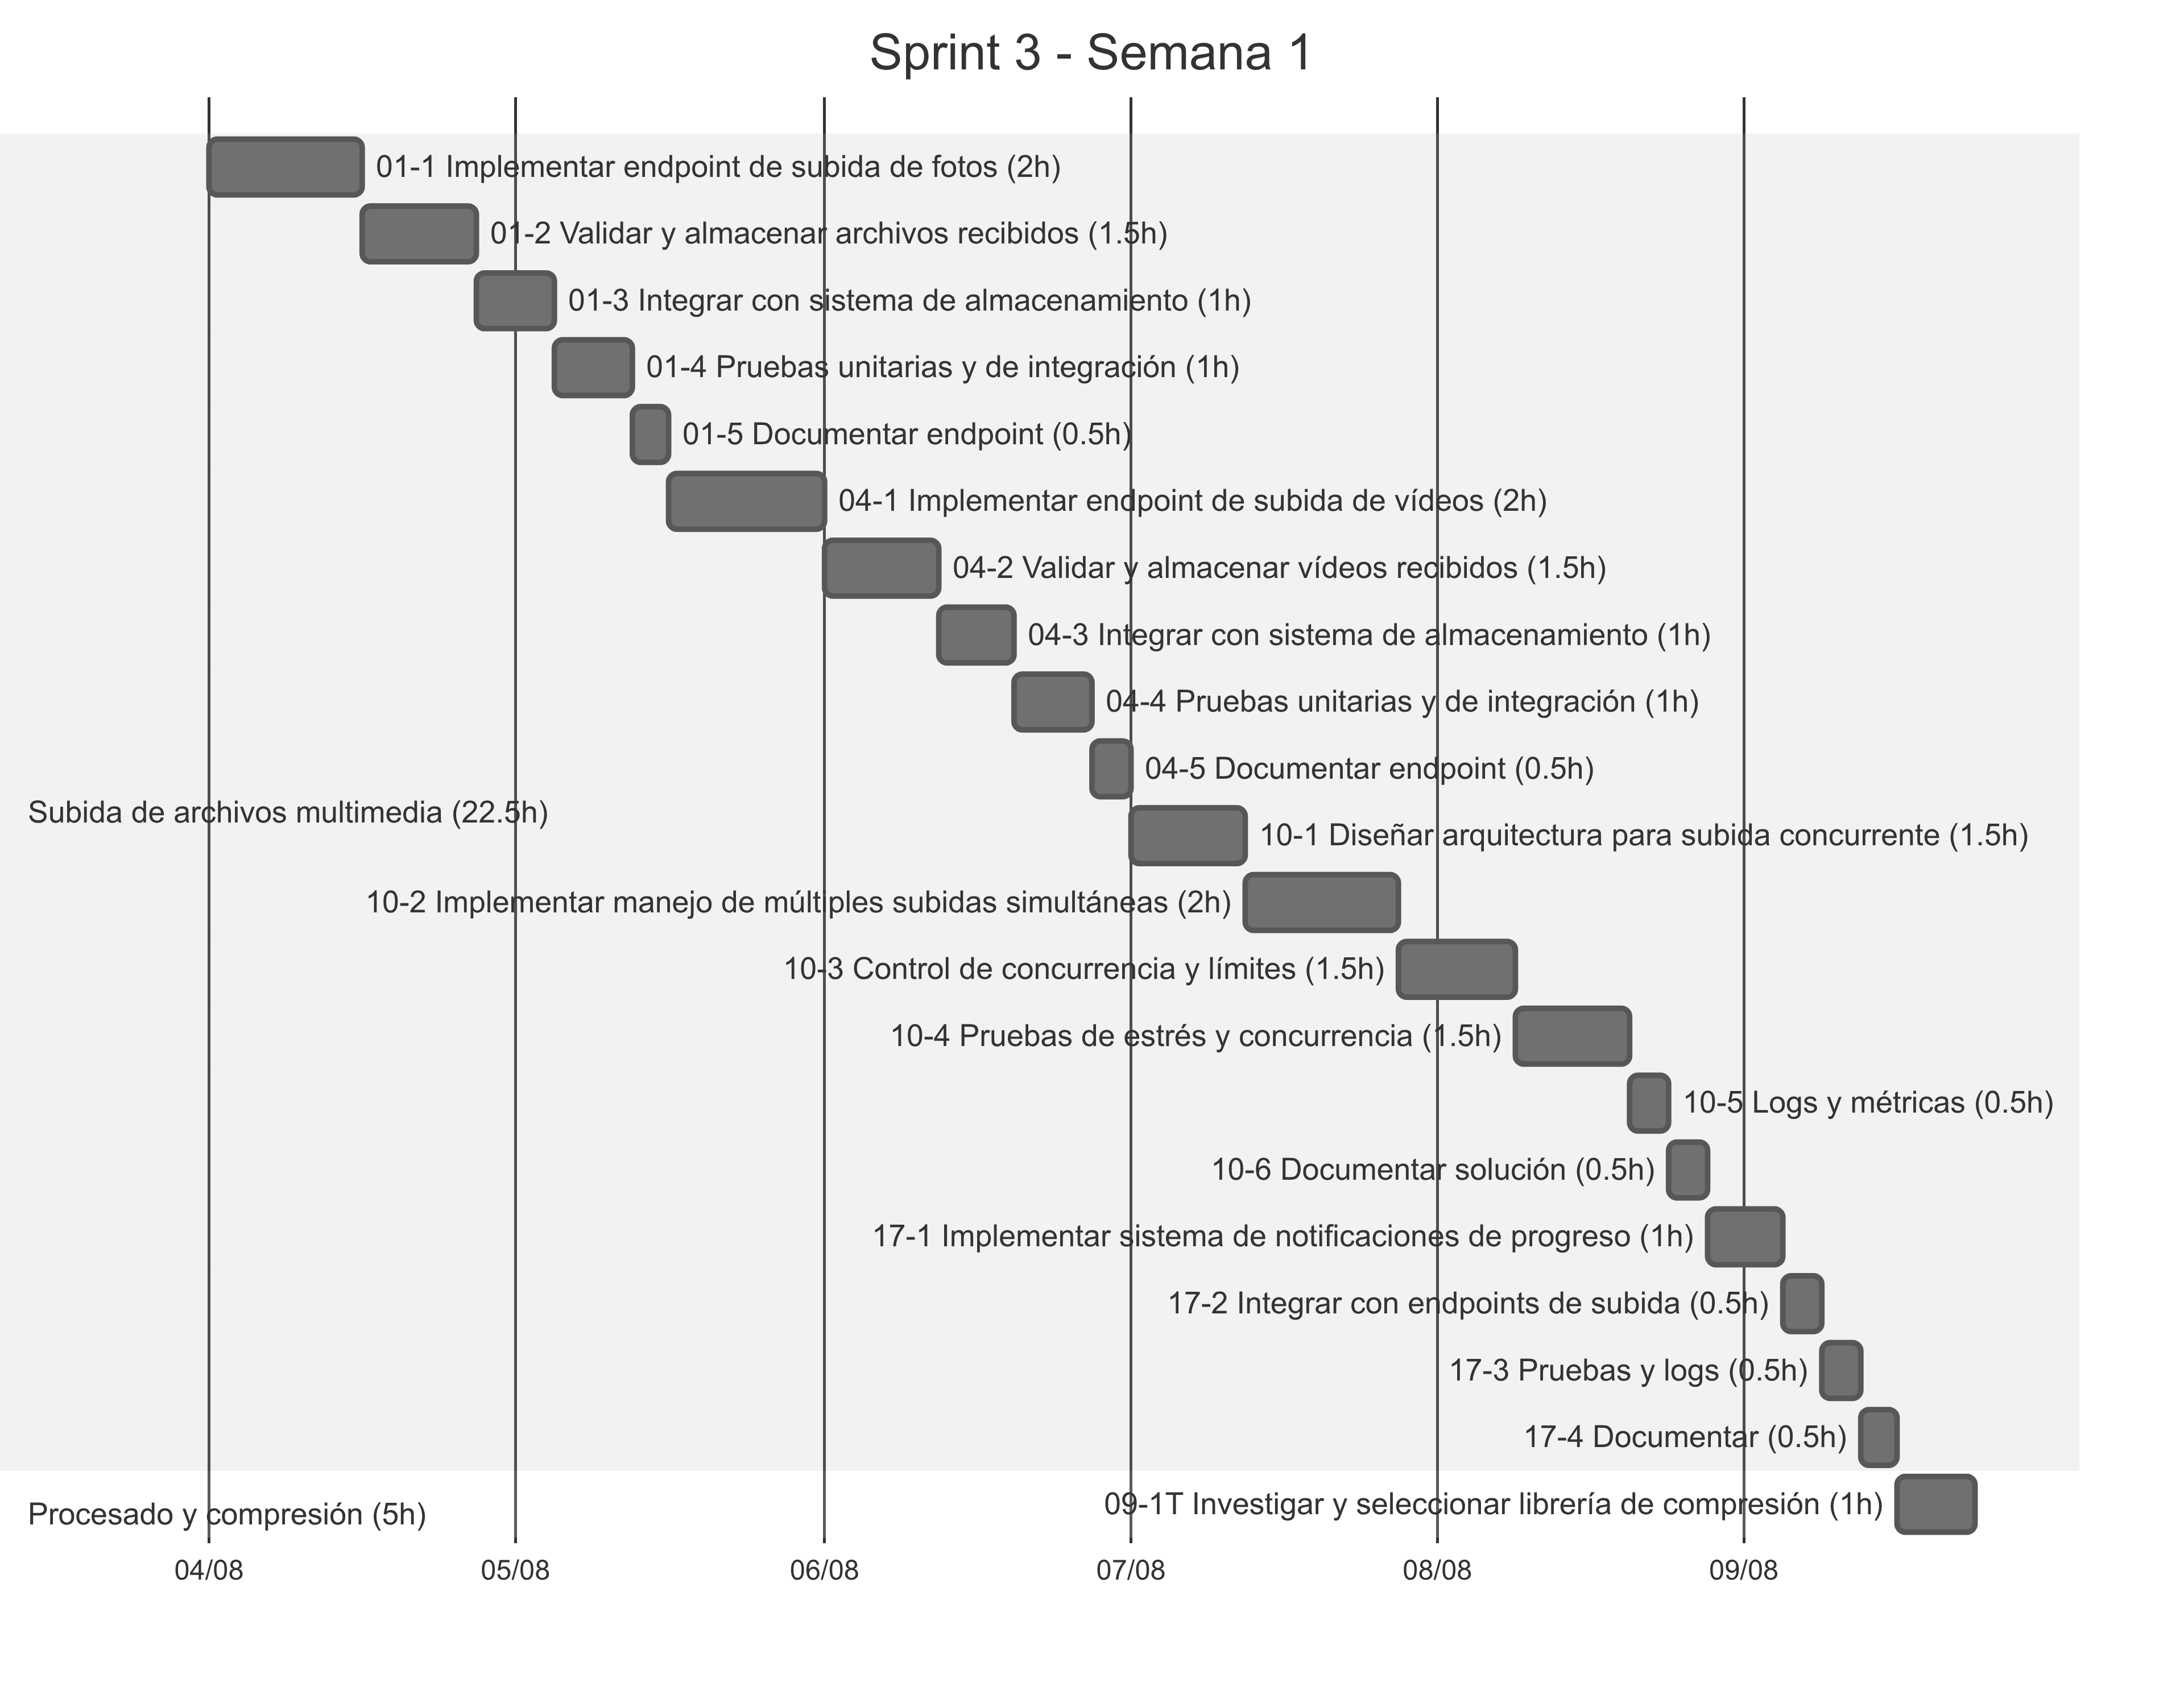
\includegraphics[width=0.8\textwidth]{assets/sprint3/week1-gantt.png}
    \end{center}
    \caption{Diagrama de Gantt de las tareas de la primera semana del sprint 3}\label{fig:gantt-sprint3-week1}
\end{figure}


\begin{figure}[H]
    \begin{center}
        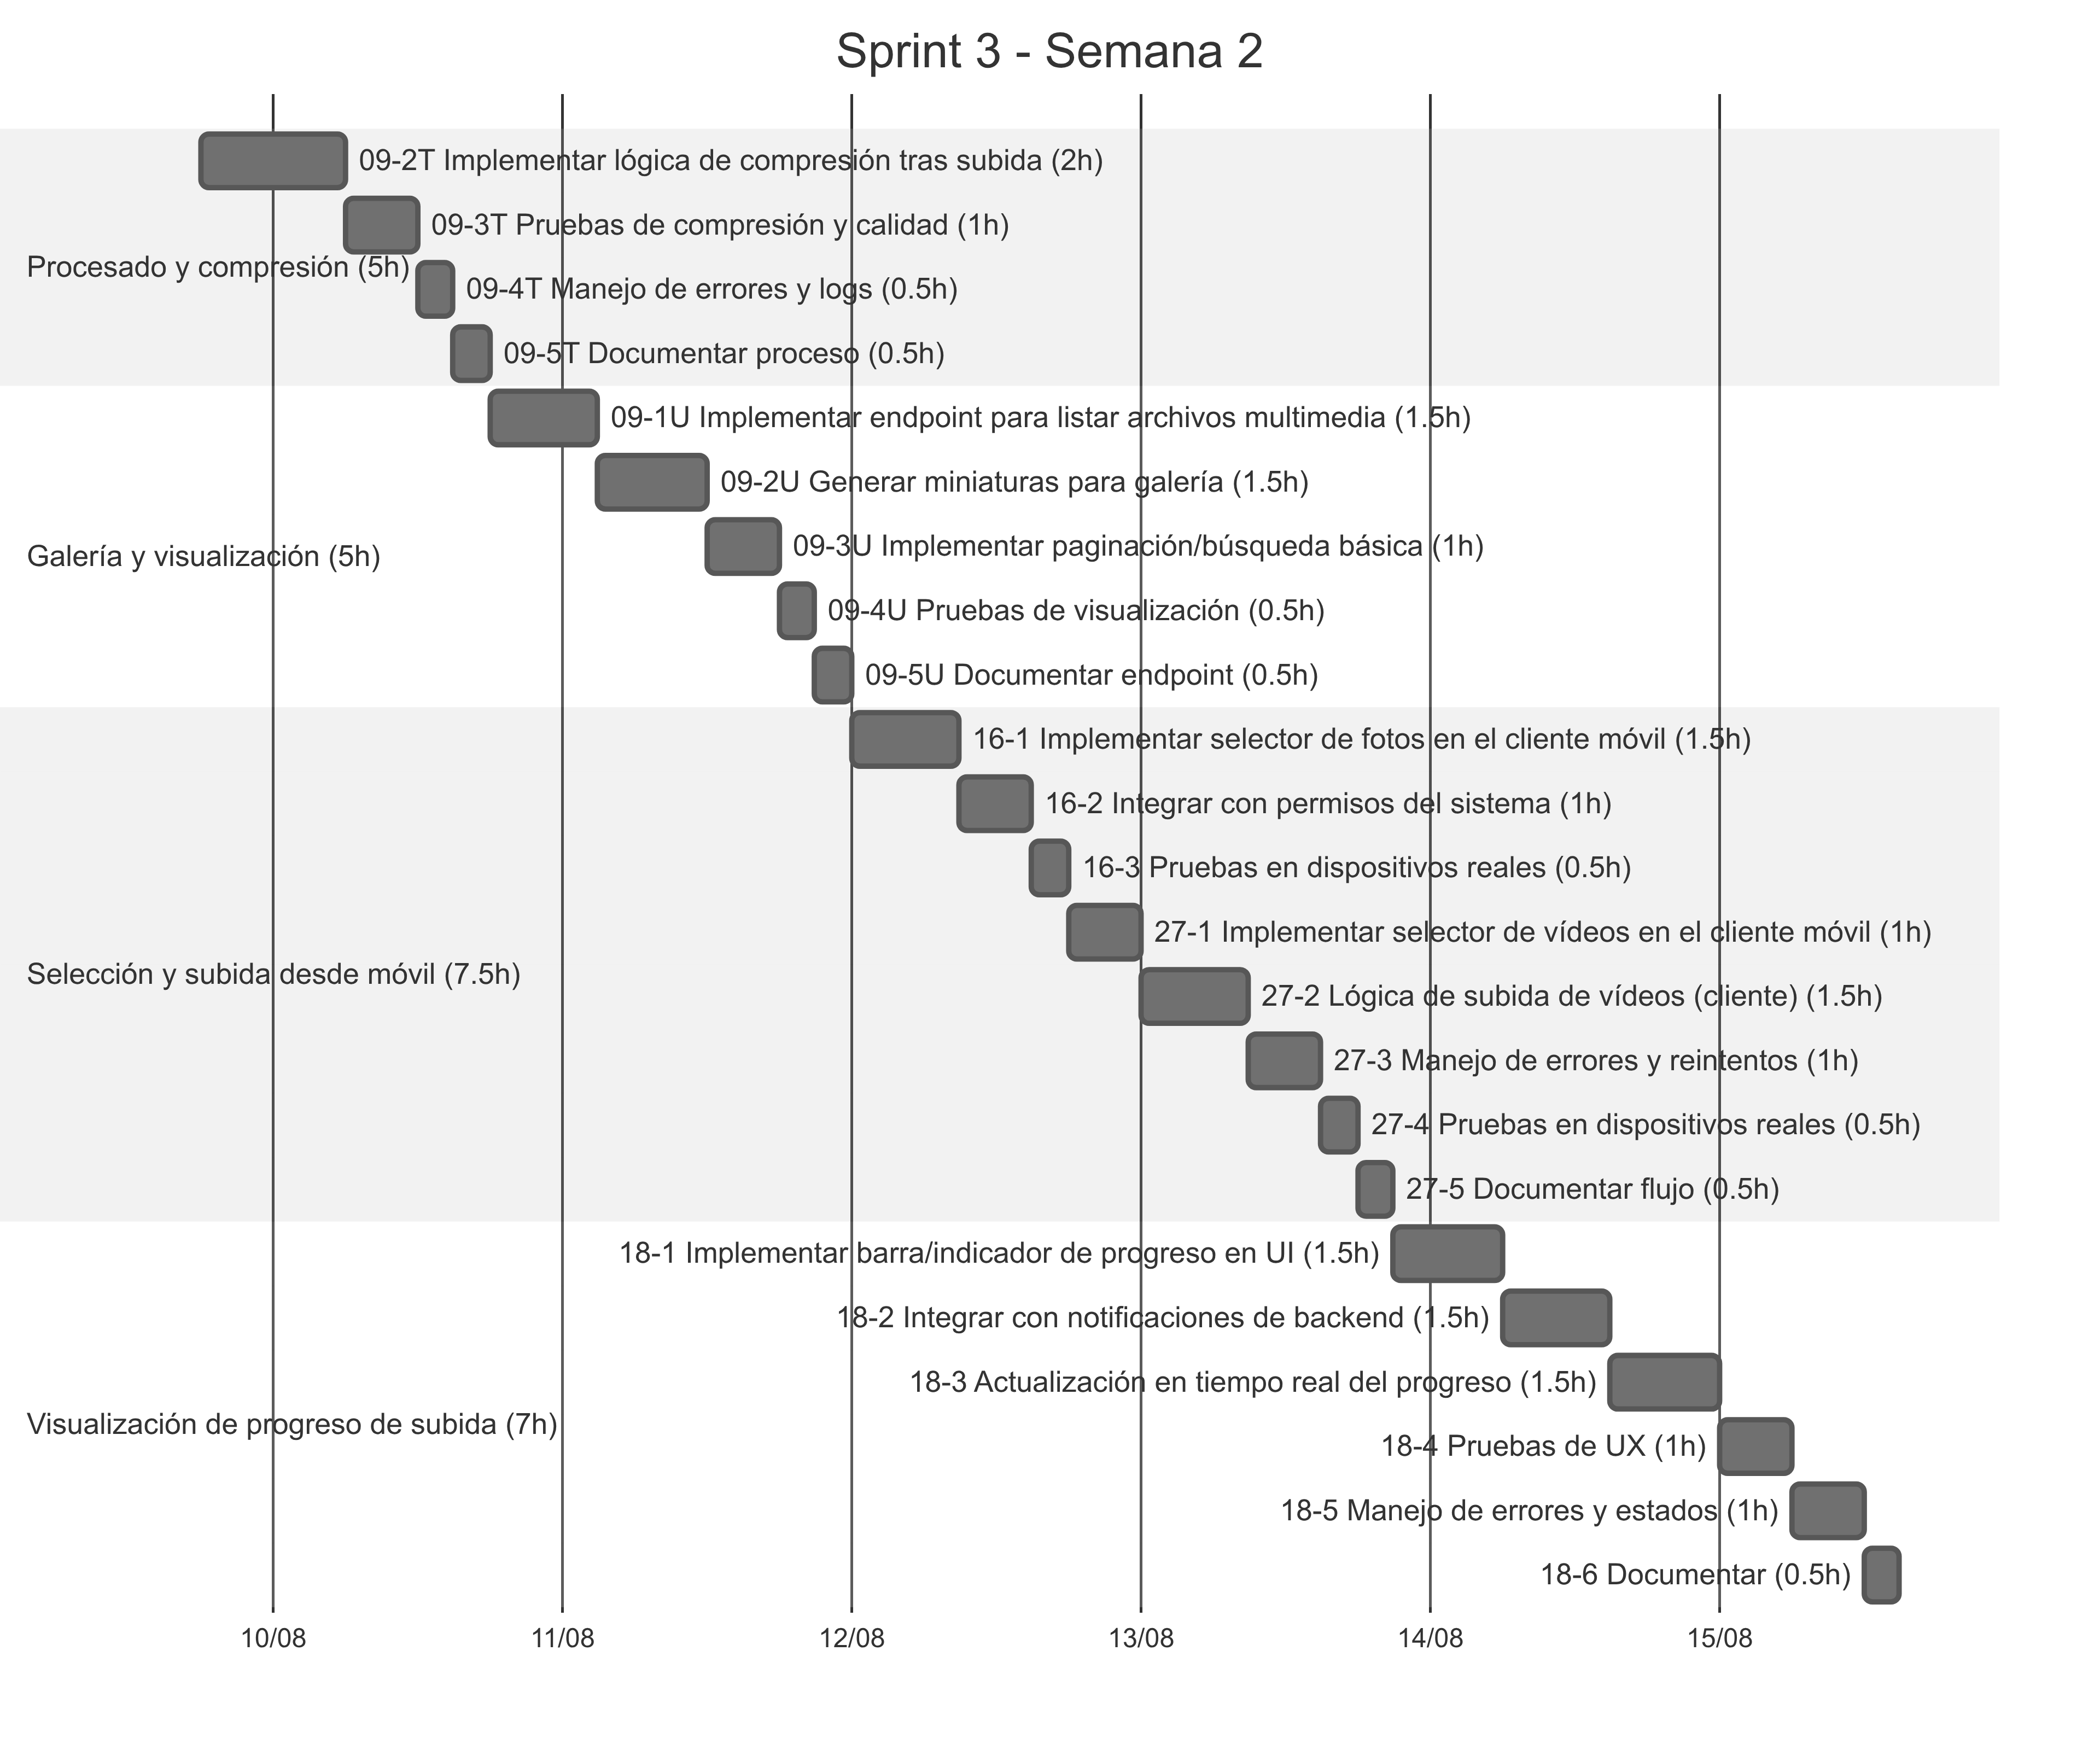
\includegraphics[width=0.8\textwidth]{assets/sprint3/week2-gantt.png}
    \end{center}
    \caption{Diagrama de Gantt de las tareas de la segunda semana del sprint 3}\label{fig:gantt-sprint3-week2}
\end{figure}

En este sprint se han priorizado las tareas relacionadas principalmente con el procesado multimedia en el servidor, dado que en el anterior sprint el enfoque estuvo en el desarrollo de la aplicación móvil.

Las tareas relacionadas con la aplicación móvil de este sprint se centran principalmente en integrar los cambios implementados en el servidor.
Se realiza de esta manera para que al finalizar el sprint 3 tengamos un producto con más valor, puesto que el usuario tendrá la posibilidad de subir fotos y vídeos desde su móvil, que serán procesados en el servidor y podrán visualizarse en una galería online.

\subsection{Detalles de implementación}
La implementación de la subida de archivos multimedia se ha realizado en dos pasos, primero se ha implementado una subida de archivos sencilla, la cual permite subir archivos multimedia al servidor habiendo iniciado sesión, guardando los archivos en MinIO y guardando los metadatos en la base de datos asociados al usuario autenticado.

El flujo que se ha seguido en la implementación ha sido el siguiente:
\begin{figure}[H]
    \begin{center}
        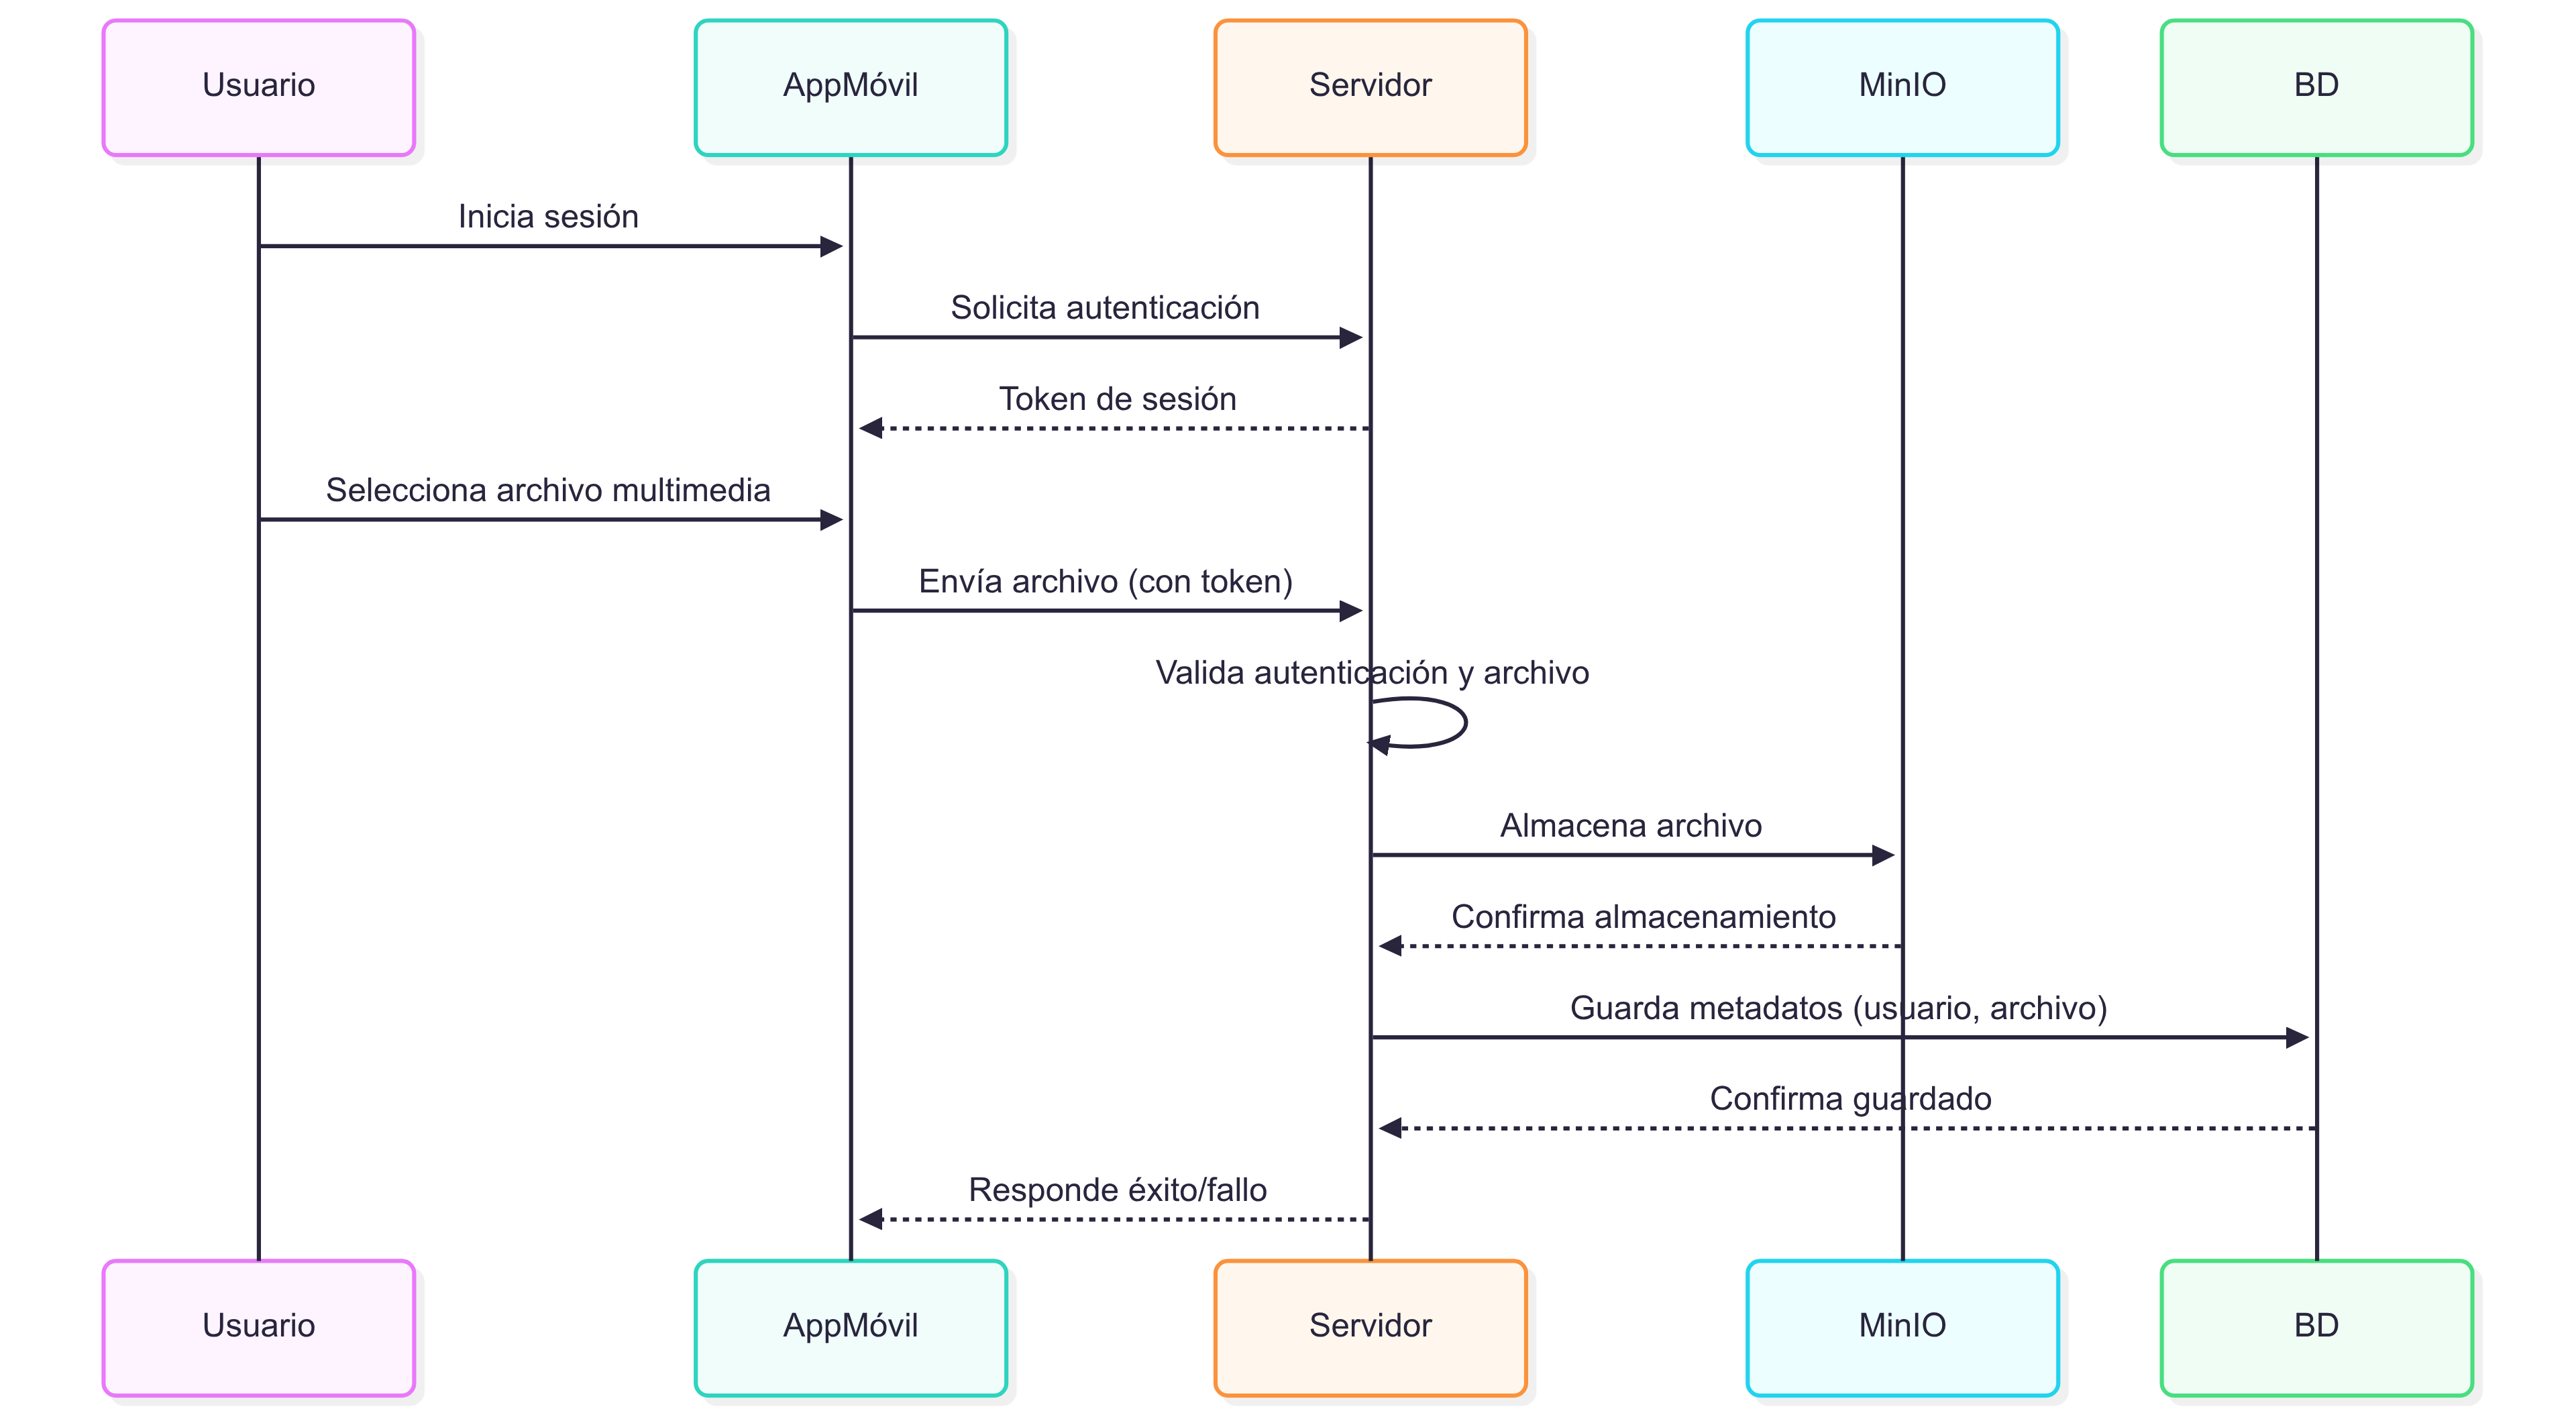
\includegraphics[width=0.95\textwidth]{assets/sprint3/diagrama-subida-archivos.png}
    \end{center}
    \caption{Diagrama de flujo de subida de archivos multimedia}\label{fig:diagrama-flujo-subida-archivos}
\end{figure}


